% !TEX program = xelatex
% Курсовой отчет ВШЭ ФКН — ГОСТ-стиль
% Компилируется через XeLaTeX:
%     xelatex main.tex
%     xelatex main.tex   (двойной проход для оглавления)

\documentclass[a4paper,14pt]{extreport}

% ===== Шрифты и язык =====
\usepackage{fontspec}
\usepackage{polyglossia}
\setdefaultlanguage{russian}
\setotherlanguage{english}

\setmainfont{Times New Roman}
\setsansfont{Arial}
\setmonofont{Consolas}
\newfontfamily\cyrillicfonttt{Consolas}

% ===== Поля по ГОСТ Р 7.0.97-2016 =====
\usepackage[
  a4paper,
  left=30mm, right=15mm, top=20mm, bottom=20mm,
  headsep=10mm, footskip=12mm
]{geometry}

% ===== Межстрочный интервал =====
\usepackage{setspace}
\onehalfspacing      % 1.5 line spacing

% ===== Абзацный отступ =====
\usepackage{indentfirst}
\setlength{\parindent}{1.25cm}
\setlength{\parskip}{0pt}

% ===== Заголовки разделов =====
\usepackage{titlesec}
\titleformat{\chapter}[block]
  {\normalfont\fontsize{14}{16}\bfseries\centering}
  {\thechapter.}
  {0.5em}
  {\MakeUppercase}
\titleformat{\section}[block]
  {\normalfont\fontsize{14}{16}\bfseries}
  {\thesection.}
  {0.5em}
  {}
\titleformat{\subsection}[block]
  {\normalfont\fontsize{14}{16}\bfseries\itshape}
  {\thesubsection.}
  {0.5em}
  {}
\titlespacing{\chapter}{0pt}{0pt}{12pt}
\titlespacing{\section}{\parindent}{12pt}{6pt}
\titlespacing{\subsection}{\parindent}{8pt}{4pt}

% Глава начинается с новой страницы, без слова "Глава"
\renewcommand{\chaptername}{}
\renewcommand{\thechapter}{\arabic{chapter}}

% ===== Нумерация страниц снизу по центру =====
% (используется встроенный стиль plain — он сам по себе дает страничную нумерацию)
\pagestyle{plain}

% ===== Графика, таблицы =====
\usepackage{graphicx}
\usepackage{float}  % allows [H] placement option for figures and tables
\graphicspath{{./}}
\usepackage{caption}
\captionsetup[figure]{labelformat=empty, labelsep=none, font=small,
  justification=centerlast, singlelinecheck=false}
\captionsetup[table]{labelformat=empty, labelsep=none, font=small,
  justification=raggedright, singlelinecheck=false}

\usepackage{array}
\usepackage{tabularx}
\usepackage{booktabs}
\usepackage{multirow}
\usepackage{longtable}
\renewcommand{\arraystretch}{1.2}
\newcolumntype{L}[1]{>{\raggedright\arraybackslash}p{#1}}
\newcolumntype{C}[1]{>{\centering\arraybackslash}p{#1}}
\newcolumntype{R}[1]{>{\raggedleft\arraybackslash}p{#1}}

% ===== Список источников =====
\usepackage{enumitem}
\setlist[enumerate]{leftmargin=*, itemsep=2pt, topsep=4pt}

% ===== Гиперссылки =====
\usepackage[
  unicode, hidelinks, breaklinks=true,
  pdftitle={Анализ алгоритмов решения задачи mTSP},
  pdfauthor={Студент Программная инженерия},
]{hyperref}
% URL-адреса печатаются тем же шрифтом, что окружающий текст
% (без typewriter и без цветовой подсветки --- ссылка читается как
%  обычная часть строки списка литературы).
\urlstyle{same}

% ===== Вспомогательные =====
\usepackage{ragged2e}
\usepackage{microtype}
\usepackage{amsmath,amssymb,amstext}  % \text{}, \mathrm{}, \Theta, \Omega in math mode
\usepackage[table]{xcolor}  % \rowcolor for table row highlighting
\definecolor{passrow}{gray}{0.93}  % subtle gray for rows passing the practical filter
\usepackage{placeins}  % \FloatBarrier

% Allow line breaks in \texttt{} on common separators (_ . / -)
\usepackage{xpatch}
\makeatletter
\let\old@texttt\texttt
\renewcommand{\texttt}[1]{{\sloppy\hyphenchar\font=\m@ne\old@texttt{#1}}}
\makeatother
% Better line breaking inside paragraphs
\sloppy
\emergencystretch=3em

% ===== Команды для удобства =====
\newcommand{\sectiontitle}[1]{%
  \begin{center}\textbf{\MakeUppercase{#1}}\end{center}\par\bigskip}

% Чтобы chapter не печатал слово "Глава 1" а только "1."
\makeatletter
\renewcommand{\@makechapterhead}[1]{%
  \vspace*{0pt}%
  {\centering\normalfont\fontsize{14}{16}\bfseries
   \ifnum\value{chapter}>0
     \thechapter.\quad
   \fi
   \MakeUppercase{#1}\par\nobreak}%
  \vspace{12pt}%
}
\renewcommand{\@makeschapterhead}[1]{%
  \vspace*{0pt}%
  {\centering\normalfont\fontsize{14}{16}\bfseries
   \MakeUppercase{#1}\par\nobreak}%
  \vspace{12pt}%
}
\makeatother

\begin{document}

% =================================================================
% ТИТУЛЬНЫЙ ЛИСТ
% =================================================================
\begin{titlepage}
\thispagestyle{empty}
\begin{center}
\textbf{ПРАВИТЕЛЬСТВО РОССИЙСКОЙ ФЕДЕРАЦИИ}\\
\textbf{НАЦИОНАЛЬНЫЙ ИССЛЕДОВАТЕЛЬСКИЙ УНИВЕРСИТЕТ}\\
\textbf{«ВЫСШАЯ ШКОЛА ЭКОНОМИКИ»}\\[4pt]
Факультет компьютерных наук\\
Образовательная программа «Программная инженерия»
\end{center}

\vspace{1em}
\begin{center}
УДК 004.023
\end{center}

\vspace{2em}
\begin{center}
\textbf{ОТЧЕТ}\\[2pt]
по исследовательскому курсовому проекту\\[14pt]

на тему\\
\textbf{«Оптимизация алгоритмов маршрутизации на~примере задачи\\
нескольких коммивояжеров»}\\[14pt]

по направлению подготовки бакалавров\\
09.03.04 «Программная инженерия»
\end{center}

\vspace{3em}
\begin{flushright}
\begin{minipage}{8cm}
Выполнил\\
студент группы БПИ246\\
образовательной программы\\
09.03.04 «Программная инженерия»\\[6pt]
Купцов Денис Дмитриевич\\[18pt]
Научный руководитель\\
Ермаков Андрей Максимович
\end{minipage}
\end{flushright}

\vfill
\begin{center}
Москва 2026
\end{center}
\end{titlepage}

% =================================================================
% РЕФЕРАТ
% =================================================================
\sectiontitle{Реферат}

Отчет 104~с., 17~рис., 24~табл., 53~источн., 8~прил.

\medskip

\textbf{Объект исследования}~--- эвристические алгоритмы решения задачи о нескольких коммивояжерах (multiple Traveling Salesman Problem, mTSP) на инстансах до~100\,000~узлов в~условиях ограниченного лимита времени.

\textbf{Цель работы}~--- спроектировать, реализовать и~экспериментально оценить собственный решатель на~базе адаптивного поиска в~больших окрестностях, сравнить его с~открытыми эталонами (LKH-3, OR-Tools, FILO2) на~стратифицированной сетке инстансов и~подтвердить выводы статистически.

\medskip
\textbf{Ключевые результаты.}
\begin{itemize}\setlength\itemsep{2pt}
\item \textbf{Большие инстансы ($N=25{-}100$\,тыс.).} ALNS-mTSP строит маршруты, равномерно распределённые между коммивояжерами; LKH-3 default отдаёт почти всю работу одному коммивояжеру~--- формально допустимое, но~непригодное для прикладной маршрутизации решение.
\item \textbf{Малые инстансы (fair-baseline).} При балансирующей настройке LKH-3 ALNS-mTSP лучше по~MINSUM на~13--18\,\%; этот разрыв служит контролем против артефакта default-LKH-3, а~не основным доказательством.
\item \textbf{Лимит времени.} ALNS-mTSP укладывается в~$T\leq 350$\,c на~всех проверенных инстансах; LKH-3 в~балансирующих режимах на~$N=25K$~--- 0/12 валидных за~30--60~мин; FILO2 в~CVRP-адаптации~--- 2/18; OR-Tools в~стандартной конфигурации не~уложился в~бюджет с~практически приемлемым решением на~$N\geq 5K$.
\item \textbf{Прямое сравнение на~$N=100K$~--- против FILO2.} На~12~ячейках $N\in\{50K,100K\}$ ALNS-mTSP выигрывает 9/12, в~т.\,ч.\ \textbf{6/6 на~$N=100K$} с~разрывом 5--30\,\% по~MINSUM.
\item \textbf{Сравнение со специализированными SOTA для MINMAX.} На~mTSPLib ($n\leq 100$) HGA~[35] и~He-Hao~MA~[29] доминируют по~makespan; на~$N\geq 25K$ их~эталонные реализации не~публикуют результатов и~в~работе не~запускались.
\end{itemize}

\medskip
\noindent\fbox{\parbox{0.97\textwidth}{\textbf{Основной результат.} В~заявленном сценарии (CPU без~GPU, $T\leq 350$\,c, $N$~до~100\,000, $n_r=m$ нетривиальных маршрутов, $\mathrm{Gini}\leq 0.05$) ALNS-mTSP проходит полный практический фильтр. Воспроизведённые открытые baseline нарушают хотя~бы одно из~условий: LKH-3 default~--- (i),~(iii); LKH-3 balanced на~$N=25K$~--- (i); OR-Tools~--- бюджет на~$N\geq 5K$; FILO2~--- (i),~(ii). Внутри допустимой области ALNS-mTSP лучше \emph{2opt+greed} (единственного открытого baseline, проходящего фильтр) на~$1.4{-}4.8\,\%$ по~MINSUM (медиана~$\approx 3.6\,\%$, табл.~5а).}}

\medskip
\textbf{Экспериментальная инфраструктура.} Собрана воспроизводимая система: генератор синтетических инстансов (6~семейств), единая C++-обёртка решателей, адаптеры WSL2 для LKH-3 и~FILO2, Python-статистика. Метрики качества и~баланса~--- по~обзору~[28]; парные сравнения~--- непараметрическими методами с~поправкой на~множественные сравнения~[39] и~bootstrap-CI~[38]; величина эффекта~--- по~[44]. Всего~--- 15~экспериментов, $\geq 2\,157$ валидных запусков на~13~конфигурациях решателей.

\textbf{Ограничения.} Часть SOTA-методов (ITSHA, MILS, нейросетевые Equity-Transformer, DPN, GLOP, DualOpt, UDC, iMTSP) не~запускалась~--- причины обсуждаются в~главе~5; направления дальнейшей работы~--- в~главе~6.

% =================================================================
% СОДЕРЖАНИЕ
% =================================================================
\newpage
\renewcommand{\contentsname}{СОДЕРЖАНИЕ}
\tableofcontents

% =================================================================
% ОПРЕДЕЛЕНИЯ
% =================================================================
\newpage
\addcontentsline{toc}{chapter}{ОПРЕДЕЛЕНИЯ, ОБОЗНАЧЕНИЯ И СОКРАЩЕНИЯ}
\sectiontitle{Определения, обозначения и сокращения}

Используемые термины и обозначения:

\begin{longtable}{|L{4.6cm}|L{9.9cm}|}
\hline
\textbf{Термин} & \textbf{Определение} \\
\hline
TSP (Traveling Salesman Problem) & Классическая задача о коммивояжере: найти кратчайший гамильтонов цикл, проходящий через каждую точку ровно один раз. NP-трудная задача. \\
\hline
mTSP (multiple TSP) & Обобщение TSP: имеется m коммивояжеров, выходящих и возвращающихся в общий депот; каждый клиент посещается ровно одним коммивояжером. \\
\hline
MINSUM & Целевая функция mTSP~--- сумма длин всех маршрутов. \\
\hline
MINMAX & Альтернативная целевая функция~--- длина самого длинного маршрута; используется для балансировки. \\
\hline
Депот (depot) & Стартовая и конечная вершина каждого маршрута. \\
\hline
Маршрут (route) & Упорядоченная последовательность вершин одного коммивояжера, начинающаяся и заканчивающаяся в депоте. \\
\hline
Тривиальный маршрут & Маршрут вида [depot, depot] (пустой) или [depot, c, depot] (один клиент); такие маршруты практически бесполезны для маршрутизации флота. \\
\hline
Вырожденное решение & Решение mTSP, в котором один коммивояжер посещает почти все клиенты, а остальные имеют тривиальные маршруты. \\
\hline
balance\_max\_avg & Диагностическая метрика равномерности маршрутов: $\mathrm{balance} = \max_s \mathrm{len}(R_s) \,/\, \overline{\mathrm{len}(R_s)} = m \cdot F_{\max}/F_{\mathrm{sum}}$. Идеал~--- 1; при~одном коммивояжере, несущем почти всю нагрузку, стремится к~$m$. \\
\hline
makespan & $F_{\max}(R) = \max_s \mathrm{len}(R_s)$~--- длина самого длинного маршрута; критерий минимизации максимума. \\
\hline
range & $\max_s \mathrm{len}(R_s) - \min_s \mathrm{len}(R_s)$~--- размах распределения длин. \\
\hline
std (длин маршрутов) & $\sqrt{\frac{1}{m} \sum_s (\mathrm{len}(R_s) - \overline{\mathrm{len}})^2}$~--- стандартное отклонение длин. \\
\hline
Gini coefficient & $G = \frac{1}{2m^2 \overline{x}} \sum_i \sum_j |x_i - x_j|$, где $x_i = \mathrm{len}(R_i)$. Принимает значения $[0,\,1{-}1/m]$. Стандартная метрика неравномерности~[28]. В~отличие от balance\_max\_avg, учитывает весь профиль распределения, не~только экстремум. \\
\hline
n\_empty & Количество маршрутов, не содержащих ни одного клиента. \\
\hline
LKH (Lin\allowbreak{}-Kernighan\allowbreak{}-Helsgaun) & Метаэвристический решатель TSP/mTSP/CVRP/CVRPTW авторства Keld Helsgaun; современная версия LKH-3. \\
\hline
TIME\_LIMIT & Параметр LKH-3, задающий предельное время работы; на больших инстанциях исполняется приближенно. \\
\hline
ALNS & Adaptive Large-Neighborhood Search~--- метаэвристика «разрушить-восстановить» с~адаптивным выбором операторов~[23,24]. \\
\hline
GLS & Guided Local Search~--- локальный поиск со~штрафами на~ребра с~большой стоимостью для побега из~локальных оптимумов. \\
\hline
POPMUSIC & Метод построения candidate-сетов через маленькие подпроблемы. \\
\hline
OR-Tools & Open-source решатель Google для задач маршрутизации (CVRP, TSP, mTSP). \\
\hline
Budget (бюджет времени) & Лимит времени, выделенный решателю; единица сравнения по производительности. \\
\hline
n, m & Число клиентов (включая депот в n) и число коммивояжеров. \\
\hline
OMP & OpenMP~--- система параллелизации для C/C++. \\
\hline
WSL & Windows Subsystem for Linux; для запуска LKH-3 и FILO2. \\
\hline
Wilcoxon signed-rank & Непараметрический парный критерий значимости (\texttt{scipy.stats.wilcoxon}); рекомендован~[34] для сравнения routing-методов. \\
\hline
Bootstrap CI & Percentile-bootstrap CI, 10\,000 ресэмплов, $\alpha = 0.05$ (\texttt{scipy.stats.bootstrap}). \\
\hline
\end{longtable}

% =================================================================
% ВВЕДЕНИЕ
% =================================================================
\newpage
\addcontentsline{toc}{chapter}{ВВЕДЕНИЕ}
\sectiontitle{Введение}

\textbf{Прикладной контекст.} Современная логистика и~планирование маршрутов курьерских и~сервисных бригад требуют эффективных инструментов работы с~большими массивами точек обслуживания. Задача о~нескольких коммивояжерах (multiple Traveling Salesman Problem, mTSP)~--- обобщение классической задачи коммивояжера на~случай $m$~агентов, выходящих из~общего депо, посещающих непересекающиеся подмножества клиентов и~возвращающихся обратно. Она встречается в~курьерской доставке, в~логистике последней мили, в~планировании работы мобильных бригад, в~маршрутизации дронов и~беспилотных транспортных средств. Особенно остро задача стоит при~росте числа точек обслуживания до~десятков и~сотен тысяч~--- такие масштабы характерны для крупных городских и~региональных операторов доставки.

\textbf{Существующие решатели и их ограничения.} Задача о~коммивояжере относится к~классу NP-трудных~[49], и~при~переходе к~нескольким исполнителям сложность только возрастает. На~инстансах с~десятками и~сотнями тысяч узлов точные методы (Concorde, Held--Karp DP~[30]) становятся неприменимыми, и~единственным практичным подходом остаются эвристики и~метаэвристики. Среди открытых решателей выделяются три эталонных:
\begin{itemize}\setlength\itemsep{1pt}
\item \textbf{LKH-3} (Lin--Kernighan--Helsgaun)~--- $k$-opt-метаэвристика с~расширением на~mTSP через штрафные функции;
\item \textbf{OR-Tools} от~Google~--- индустриальный решатель на~основе Guided Local Search;
\item \textbf{FILO2} (Accorsi, Vigo,~2024)~--- сильный CVRP-решатель, адаптируемый на~mTSP через ограничение вместимости маршрута.
\end{itemize}
Большинство публикаций сравнивают эти решатели на~$N \leq 10\,000$; на~TSP-100K даже LKH-3 требует около 8~часов на~один прогон, что нереально для прикладных условий.

\textbf{Перспективное направление: ALNS.} Адаптивный поиск в~больших окрестностях (Adaptive Large-Neighborhood Search, ALNS)~[23,24] в~сочетании с~алгоритмом имитации отжига и~candidate-set-фильтрацией хорошо показывает себя на~средних масштабах; обзоры структуры операторов и~стратегий их~выбора~--- [36,42]. Однако значительная часть существующих ALNS-реализаций ориентирована на~$N\sim 1\,000$ и~не~масштабируется до~$N=100\,000$ без~специальных инженерных приёмов: KD-tree-поиск, candidate-set, region-granular-операторы, параллельный multi-start. Таким образом, разработка собственного ALNS-решателя для крупных mTSP-инстансов и~его сравнительный анализ с~открытыми эталонами~--- актуальная задача, имеющая практическое и~научное значение.

\medskip
\textbf{Объект исследования}~--- эвристические алгоритмы решения задачи о~нескольких коммивояжерах (mTSP) на инстанциях с~$N$~до~100\,000 узлов в~условиях ограниченного бюджета времени.

\textbf{Предмет исследования}~--- собственный решатель ALNS-mTSP (модульная архитектура \texttt{src/v21/}) и его относительная эффективность по сравнению с~открытыми эталонными решателями LKH-3, OR-Tools и~FILO2 на стратифицированной сетке инстансов.

\textbf{Цель работы}~--- спроектировать, реализовать и экспериментально оценить собственный ALNS-решатель крупных mTSP-инстансов; провести систематическое сравнение с~тройкой эталонных открытых решателей и определить диапазоны параметров $(N,m,\text{геометрия})$, на которых ALNS-mTSP дает наилучший компромисс качество/время.

\textbf{Задачи исследования:}
\begin{enumerate}
\item Реализовать модульный ALNS-решатель с~четырьмя специализированными вариантами (alns\_minsum, alns\_cap, alns\_depot2m, alns\_minmax), поддерживающий $N$ до~100\,000 и $m$~до~100.
\item Собрать воспроизводимую экспериментальную инфраструктуру: генератор синтетических инстансов из~6~геометрических семейств, единая C++-обертка для всех решателей, адаптеры WSL2 для LKH-3 и FILO2, Python-скрипты статистики.
\item Провести стратифицированный бенчмарк трех масштабов ($N \leq 1\,000$; $N=25\,000$; $N \in \{50\,000,\,100\,000\}$) с корректной парной статистикой: Wilcoxon signed-rank, BCa-bootstrap CI, Holm-коррекция, Cliff's $\delta$.
\item Сравнить ALNS-mTSP с~LKH-3 в~трех режимах (default-MINSUM, balanced-MINSUM \texttt{MIN\_SIZE=-1}, balanced-MINMAX), с~OR-Tools (PATH\_CHEAPEST\_ARC + GUIDED\_LOCAL\_SEARCH) и~с FILO2 в~CVRP-адаптации.
\item Кросс-валидировать результаты на стандартном наборе mTSPLib (Necula et al.) и со специализированными SOTA для MINMAX-mTSP (HGA Mahmoudinazlou--Kwon, He--Hao MA).
\item Сформулировать рекомендации по~применимости 13~исследованных конфигураций решателей и~зафиксировать ограничения работы.
\end{enumerate}

\begin{figure}[htbp]
\centering
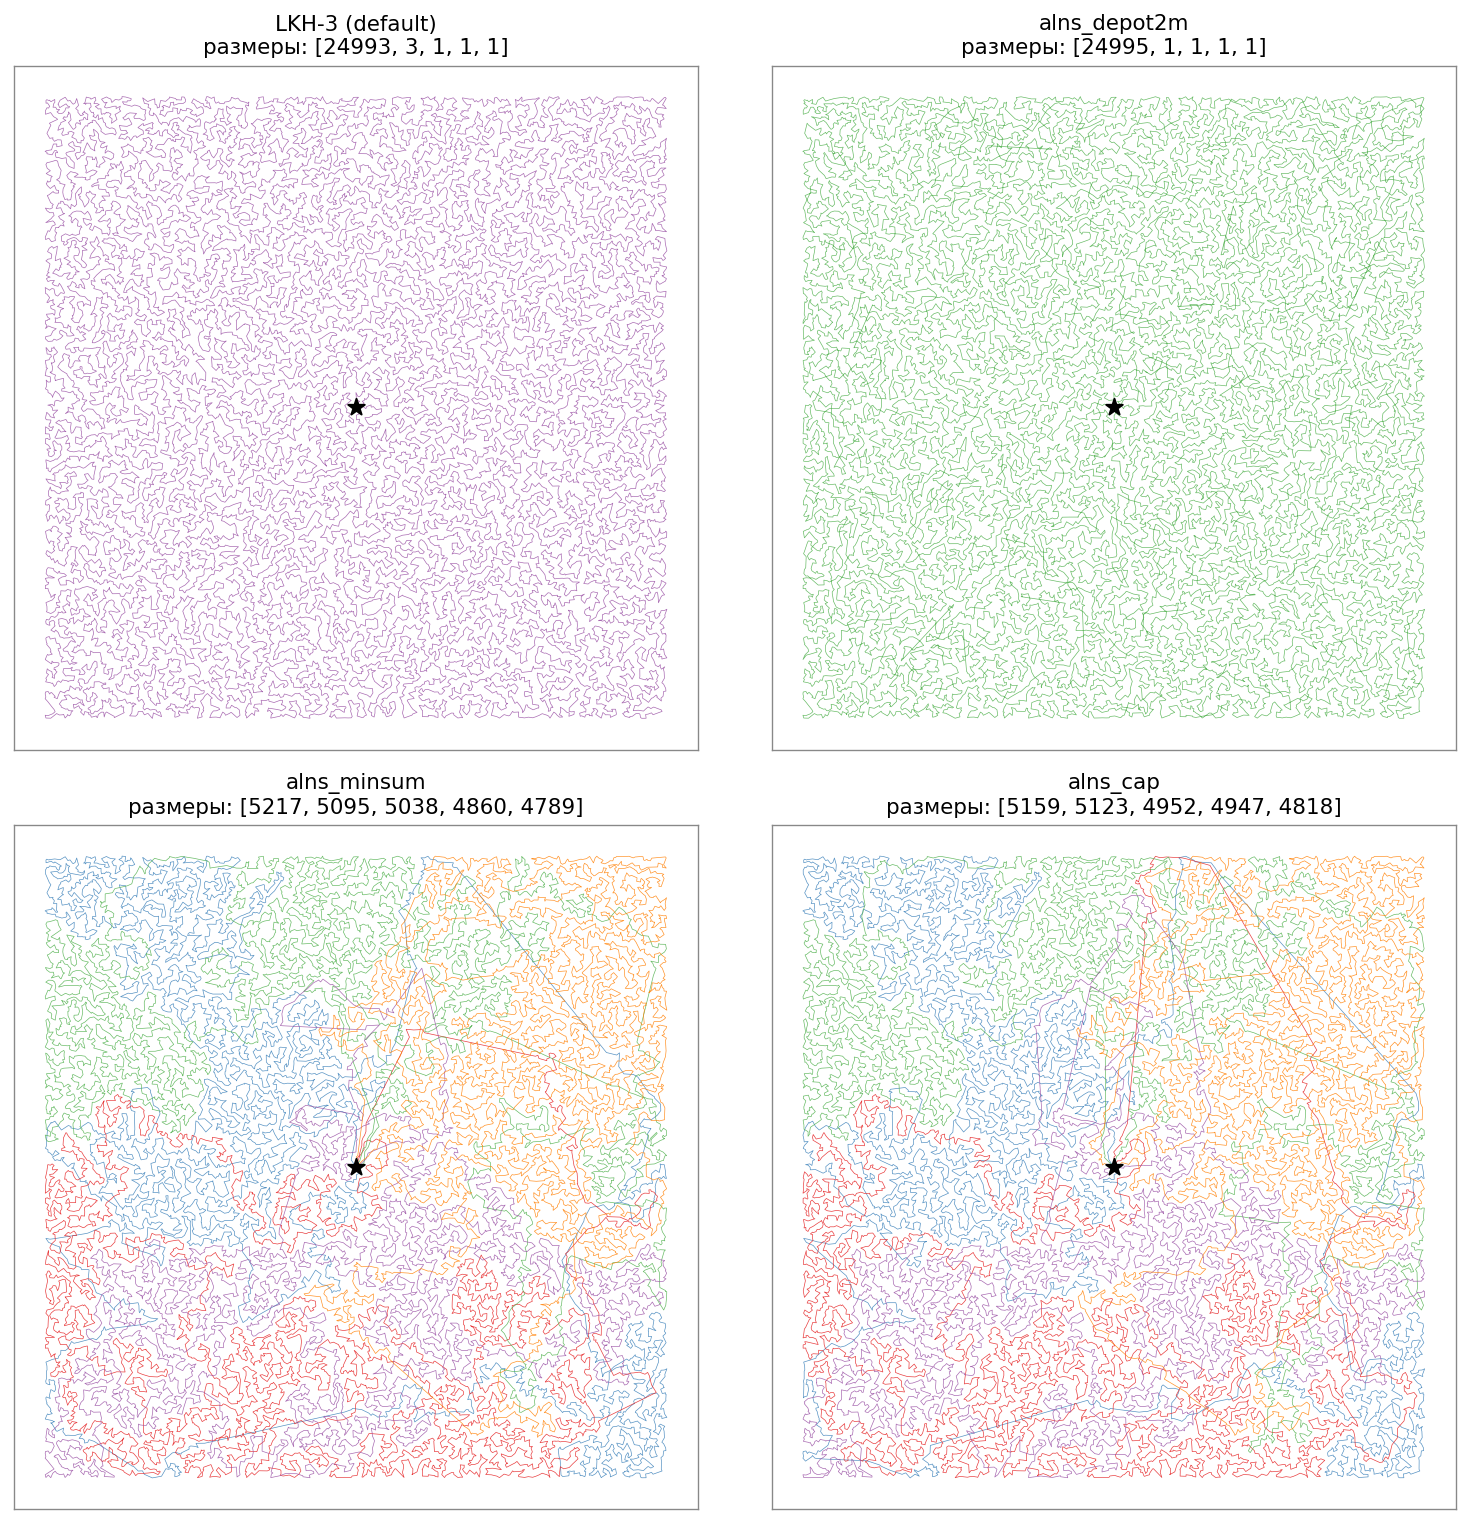
\includegraphics[width=\textwidth]{fig4_routes_compare_n25k.png}
\caption*{Рисунок~1~--- Структура маршрутов на $N=25\,000$, $m=5$ (uniform): \emph{слева}~--- вырожденные решения (LKH-3~default и~alns\_depot2m), \emph{справа}~--- сбалансированные (alns\_minsum и~alns\_minsum\_cap).}
\end{figure}

\noindent\textit{Чтение рисунка~1.} В~вырожденных решениях один коммивояжёр посещает почти все 25\,000 точек, остальные четыре маршрута тривиальны. В~сбалансированных решениях пять непересекающихся зон сравнимого размера. Это~--- центральный визуальный аргумент работы: формально-минимальная по~MINSUM конфигурация (слева) непригодна для практической маршрутизации флота, тогда как сбалансированная (справа) удовлетворяет требованию~(iii) практического фильтра.

\textbf{Гипотезы работы.} При ограниченном бюджете времени до~350 секунд на CPU собственный решатель ALNS-mTSP даёт практически применимое решение задачи о нескольких коммивояжерах на инстансах с $N$~до 100\,000 узлов~--- то есть решение, удовлетворяющее одновременно трём практическим требованиям: (i)~укладывание в заявленный лимит времени; (ii)~ровно $m$~нетривиальных маршрутов; (iii)~приемлемая балансировка длин маршрутов между коммивояжерами. Утверждение формулируется на двух уровнях.
\begin{itemize}
\item \textbf{Главная гипотеза.} В~рамках бюджета времени до~350 секунд ALNS-mTSP возвращает решения, удовлетворяющие~(i)--(iii), на~инстансах с~$N$ до~100\,000 узлов. Открытые эталонные решатели (LKH-3, OR-Tools, FILO2) в~тех~же условиях либо нарушают~(i)~--- не~укладываются в~бюджет, либо нарушают~(ii)--(iii)~--- возвращают вырожденные решения или систематически отклоняются от~заданного~$m$.
\item \textbf{Итоговая гипотеза.} В~заявленном сценарии (mTSP на~CPU без~GPU, лимит времени до~350 секунд, инстансы до~100\,000 узлов) ALNS-mTSP~--- конкурентоспособная альтернатива воспроизведённым в~работе открытым baseline. Сравнение с~нейросетевыми и~частью специализированных SOTA-методов ограничено анализом применимости по~опубликованным масштабам, требованиям к~GPU и~доступности исходного кода~--- прямое сравнение в~работе не~выполнено.
\end{itemize}

\medskip
\textit{Операциональный критерий приемлемой балансировки.} Под «приемлемой балансировкой» в~условии~(iii) понимается рабочий порог $\mathrm{Gini}\leq 0.05$ или $\mathrm{balance\_max\_avg}\leq 1.10$ на основных больших инстансах ($N\in\{25K,50K,100K\}$). Пороги используются как диагностическое правило для отделения вырожденных решений (один маршрут несёт почти всех клиентов) от равномерных. На малых инстансах ($N\leq 1\,000$) критерий смягчён до $\mathrm{balance}\leq 1.5$~--- MINSUM-оптимум на этом масштабе сам допускает тривиальные маршруты.

\begin{figure}[htbp]
\centering
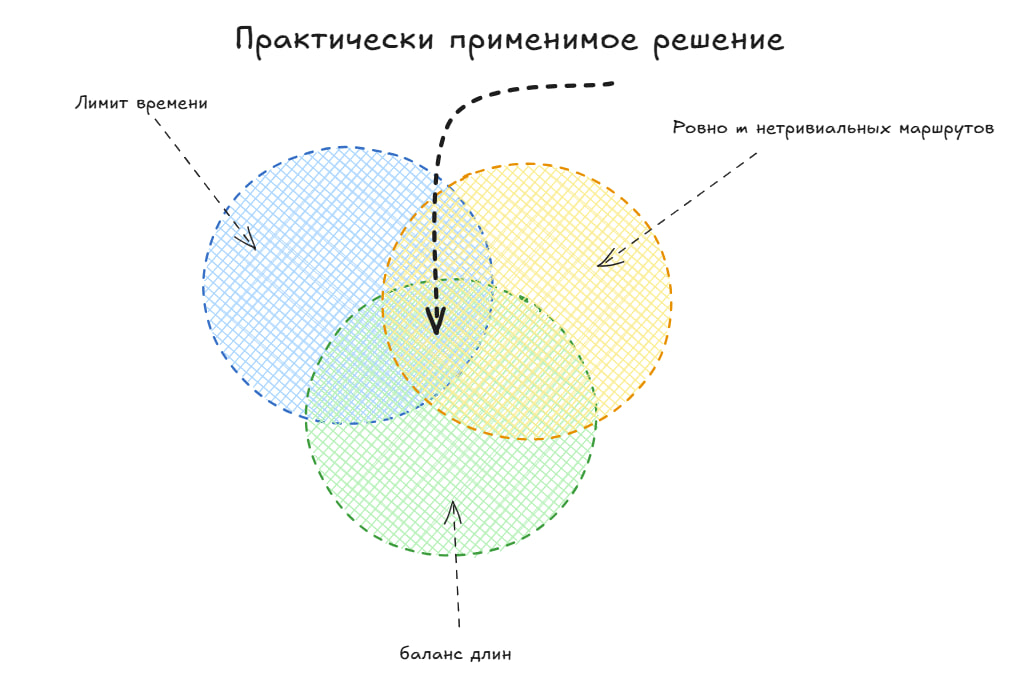
\includegraphics[width=0.80\textwidth]{fig_practical_solution.png}
\caption*{Рисунок~2~--- «Практически применимое решение» как пересечение трёх требований практического фильтра: (i)~$t\leq T_\mathrm{budget}$, (ii)~$n_r=m$ нетривиальных маршрутов, (iii)~приемлемая балансировка длин.}
\label{fig:practical-solution}
\end{figure}

\noindent Главная и итоговая гипотезы формулируются как утверждения о~попадании ALNS-mTSP в~центральную область пересечения~--- недостижимую для рассмотренных открытых эталонов в~целевом сценарии.

Сопутствующие гипотезы~H1--H6 (вырождение чистого MINSUM, поведение OR-Tools на~$N \geq 5K$, адаптивность весов ALNS, рост преимущества с~$m$, квази-линейное масштабирование по~времени, симметрия вырождения) проверяются отдельно в~разделе~4.4.

\textbf{Методологический дисклеймер о~LKH-3.} Часть таблиц использует LKH-3 в~default-конфигурации (\texttt{MTSP\_MIN\_SIZE = 1}, \texttt{MTSP\_OBJECTIVE = MINSUM}), при которой допустимы вырожденные решения с~маршрутами длиной 0~или 1~клиент.

Раздел~4.6 содержит отдельный fair-baseline-прогон LKH-3 с~балансирующими параметрами (\texttt{MIN\_SIZE = -1} и~MINMAX). Этот fair-baseline трактуется не как окончательное доказательство превосходства ALNS, а как (а)~демонстрация цены балансировки для LKH-3 и (б)~контроль того, что преимущество ALNS на малых инстансах не сводится исключительно к артефакту default-конфигурации; default-режим LKH-3~--- как иллюстрация эффекта вырождения чистого MINSUM.

\medskip
\textbf{Структура работы.}
\begin{itemize}\setlength\itemsep{1pt}
\item \emph{Глава~1}~--- обзор алгоритмов решения mTSP и~TSP, постановка задачи и теоретические оценки сложности.
\item \emph{Глава~2}~--- сравнение архитектур исследуемых решателей.
\item \emph{Глава~3}~--- экспериментальная программа: подготовка инстансов, метрики, статистические инструменты.
\item \emph{Глава~4}~--- результаты стратифицированного бенчмарка, проверка гипотез H1--H6, ablation, fair-baseline-сравнение, mTSPLib, FILO2 и~SOTA.
\item \emph{Глава~5}~--- достоверность, ограничения и риски.
\item \emph{Глава~6}~--- заключение и направления дальнейшей работы.
\item \emph{Приложения~А--З}~--- детали архитектуры ALNS-mTSP, обоснование вырождения чистого MINSUM, постпроцессинговые артефакты, эволюция исторической \texttt{lkh-wrapper}-линии (v1\dots v21), полная теоретическая сложность и расширенный обзор внешних SOTA-решателей.
\end{itemize}

% =================================================================
% Глава 1
% =================================================================
\chapter{Обзор алгоритмов решения mTSP и TSP}

В~главе рассмотрены ключевые подходы к решению mTSP: точные методы, классические эвристики, метаэвристики и нейросетевые подходы. Отмечены особенности каждого класса на больших инстансах ($N \geq 25\,000$), существенные для экспериментального сравнения. Глава завершается оценкой временной сложности.

\section{Постановка задачи mTSP}
\label{sec:mtsp-statement}

Обозначим через~$0$ депот, через $C=\{1,\dots,n-1\}$~--- множество клиентов, и положим $V=\{0\}\cup C$, $|V|=n$. На полном множестве пар~$V\times V$ задана весовая функция~$w:V\times V\to\mathbb{R}_{\geq 0}$; в~настоящей работе $w(u,v)=\lVert p_u-p_v\rVert_2$, где $p_u\in\mathbb{R}^2$~--- координата вершины~$u$ на плоскости $[0,100]^2$. Каждой инстанции соответствует полный взвешенный граф
\begin{equation}
G=(V,\,E,\,w),\qquad E=\bigl\{(u,v):u,v\in V,\;u\neq v\bigr\}.
\label{eq:graph}
\end{equation}
Дополнительно задано число агентов~$m\in\mathbb{N}$, $m\leq n-1$.

Под \emph{маршрутом} агента~$s\in\{1,\dots,m\}$ понимается упорядоченная последовательность
\[
R_s=\bigl(v^{(s)}_0,\,v^{(s)}_1,\,\dots,\,v^{(s)}_{\ell_s},\,v^{(s)}_{\ell_s+1}\bigr),\qquad v^{(s)}_0=v^{(s)}_{\ell_s+1}=0,
\]
длина которой определяется как
\begin{equation}
\mathrm{len}(R_s)=\sum_{i=0}^{\ell_s}w\!\bigl(v^{(s)}_i,\,v^{(s)}_{i+1}\bigr).
\label{eq:route-length}
\end{equation}

\medskip
\noindent\textbf{Определение 1} (допустимое решение mTSP)\textbf{.} \emph{Набор $R=\{R_1,\dots,R_m\}$ называется допустимым решением задачи mTSP, если:} (а)~\emph{каждый маршрут начинается и заканчивается в депоте; (б)~каждый клиент $c\in C$ принадлежит ровно одному маршруту; (в)~внутри каждого маршрута клиенты не повторяются.}

\medskip
В работе рассматриваются две основные целевые функции:
\begin{align}
F_{\mathrm{sum}}(R) &= \sum_{s=1}^{m}\mathrm{len}(R_s)\;\;\longrightarrow\;\;\min \qquad\text{(MINSUM),}\label{eq:minsum}\\
F_{\max}(R) &= \max_{s=1,\dots,m}\mathrm{len}(R_s)\;\;\longrightarrow\;\;\min \qquad\text{(MINMAX).}\label{eq:minmax}
\end{align}
Если все длины $\mathrm{len}(R_s)$ равны, обе целевые функции совпадают с~точностью до~множителя $1/m$; в~общем случае оптимумы~(\ref{eq:minsum}) и~(\ref{eq:minmax}) разнесены, причём степень их~рассогласования зависит от~геометрии инстанса и~числа агентов~--- количественный worst-case-анализ соответствия min-sum и~min-max в~маршрутизации приведён в~[27].

\medskip
\noindent\textbf{О вырождении в чистом MINSUM.} Определение~1 не требует $\mathrm{len}(R_s)>0$, т.\,е.\ допускает маршруты вида $R_s=(0,0)$ (пустой) или $R_s=(0,c,0)$ (синглтон). Без дополнительных ограничений (\texttt{MIN\_SIZE}, \texttt{MAX\_SIZE}, capacity) минимум~(\ref{eq:minsum}) часто достигается на конфигурации, в которой один маршрут проходит по всем клиентам, а остальные $m-1$~маршрутов тривиальны~--- такое решение формально допустимо, но непригодно для маршрутизации флота. Эмпирическая проверка этого свойства приведена в~разделе~4.4 (H1) и обоснование~--- в~Прил.~Б.

\begin{figure}[htbp]
\centering
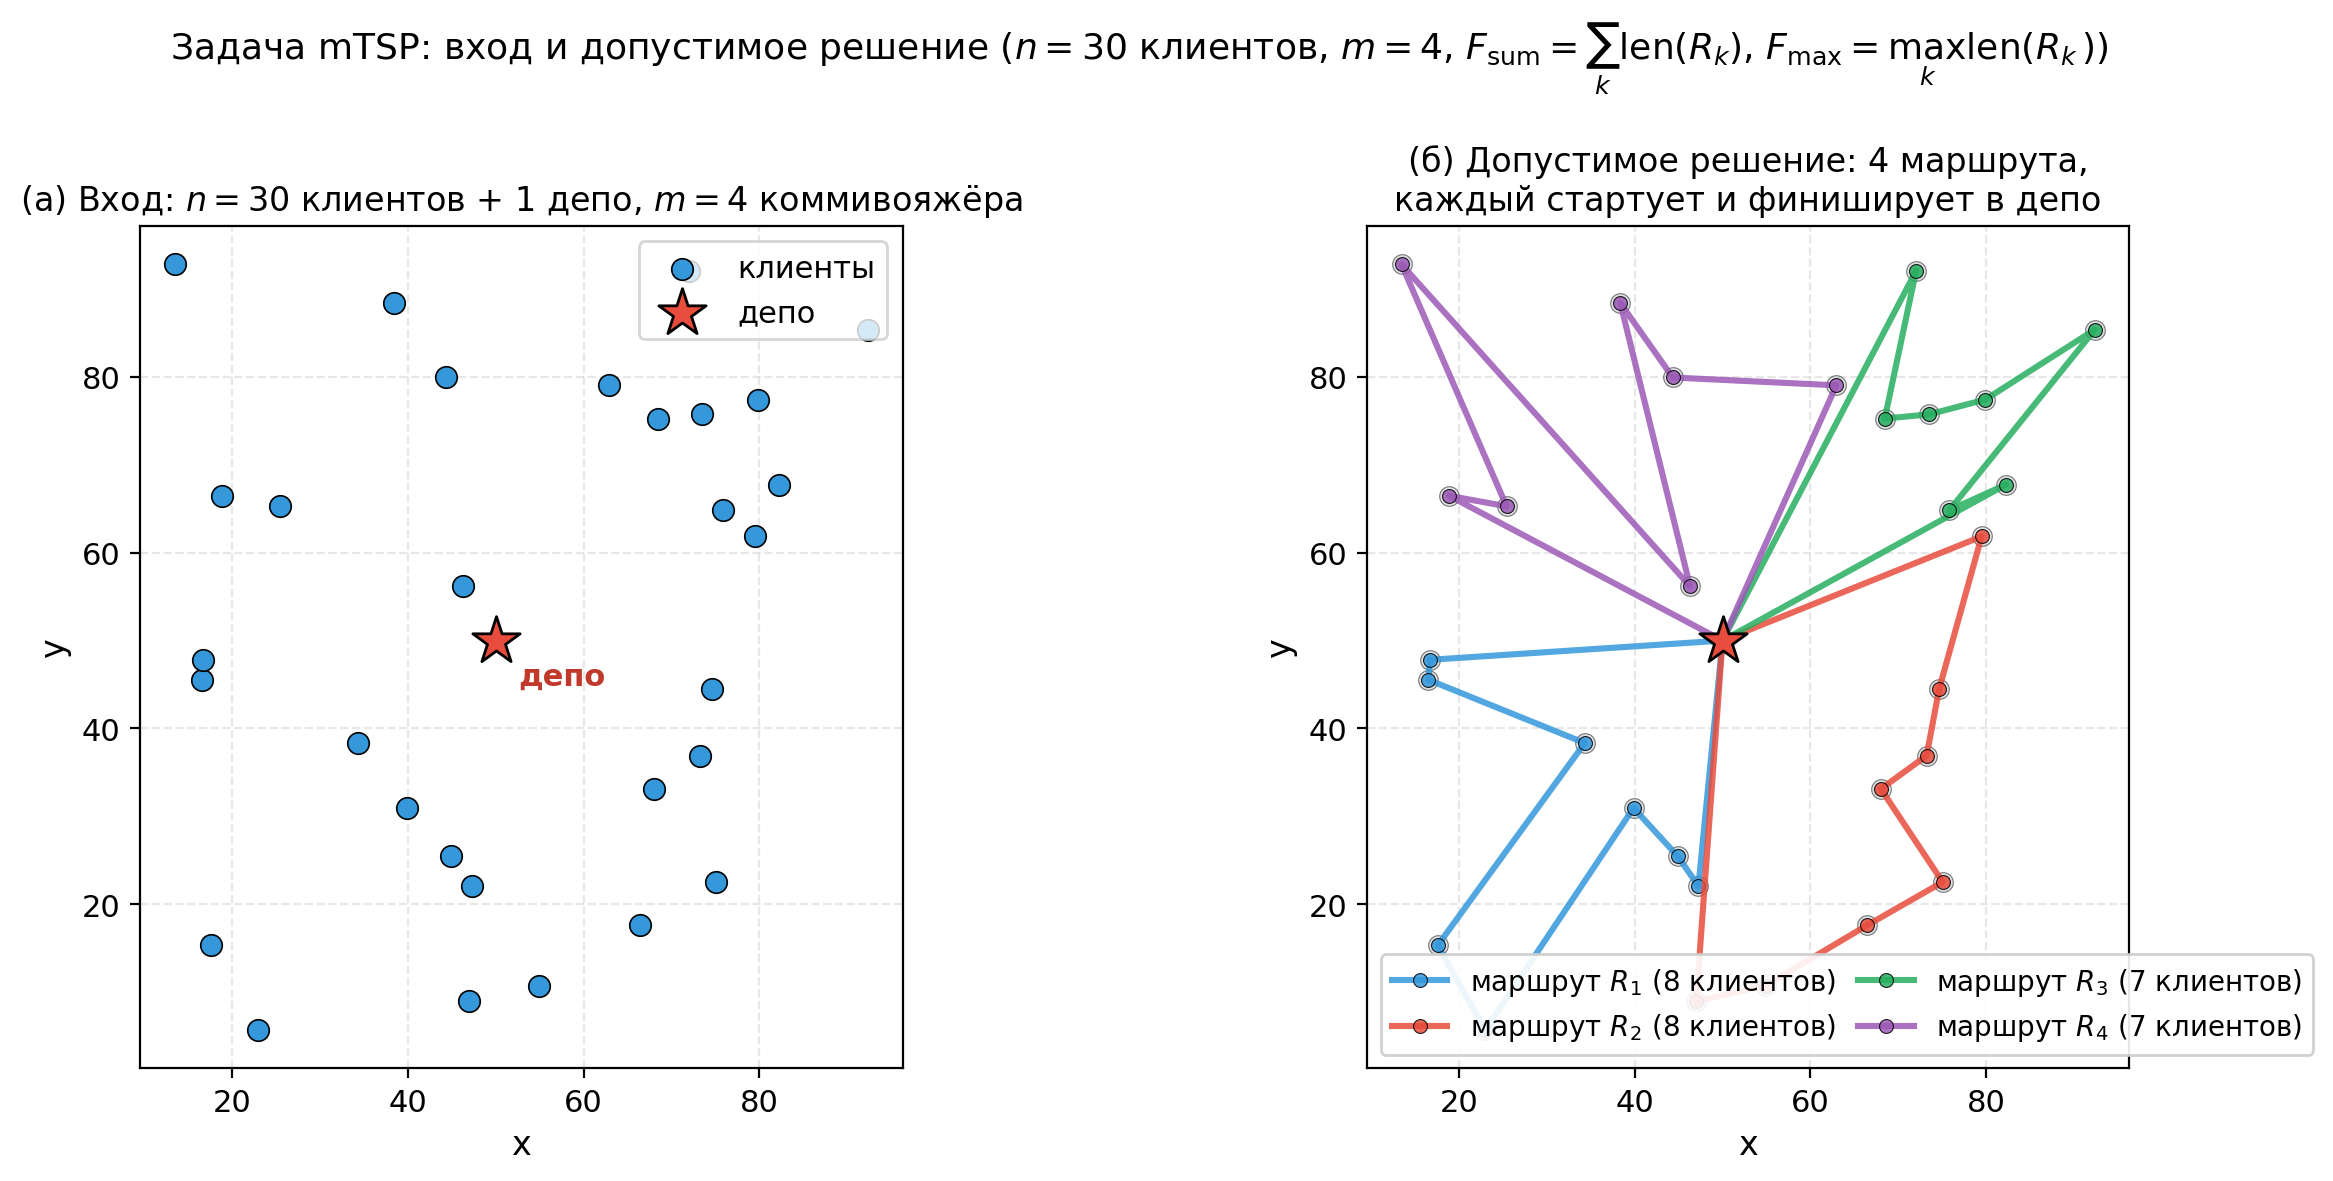
\includegraphics[width=0.96\textwidth]{fig_mtsp_problem.png}
\caption*{Рисунок 3~--- Иллюстрация постановки mTSP на маленькой инстанции ($n=30$ клиентов, $m=4$ коммивояжера, депо в~центре поля $100\times 100$). \emph{Слева~(а)}: вход~--- множество $V = \{0, 1, \dots, 30\}$, где 0~--- депо (красная звезда), $1\dots 30$~--- клиенты (синие точки). \emph{Справа~(б)}: одно из допустимых решений~--- 4~маршрута $R_1, R_2, R_3, R_4$, каждый начинается и заканчивается в~депо, посещает $7\dots 8$ клиентов; цвет маршрута соответствует своему коммивояжеру. Целевые функции: $F_{\mathrm{sum}}(R) = \sum_{k=1}^{m} \mathrm{len}(R_k)$ (MINSUM) и $F_{\max}(R) = \max_k \mathrm{len}(R_k)$ (MINMAX).}
\label{fig:mtsp-problem}
\end{figure}

\section{Точные методы и Concorde}

Программа Concorde~[3,4] (Applegate, Bixby, Chvátal, Cook)~--- золотой стандарт точных решателей TSP, работающий на~стандартных инстанциях TSPLIB~[26]. Concorde находит доказуемо оптимальные решения. Однако его применимость ограничена малыми и~средними~$N$: по~публичным данным, на~инстанции с~$n=85\,900$ узлов Concorde тратит порядка 136~CPU-лет; на~случайных евклидовых инстанциях с~$n>10\,000$ он, как правило, не~завершается в~разумное время. Аналогично динамическое программирование Held--Karp~[30] требует $\Theta(n^2\cdot 2^n)$ времени и~$\Theta(n\cdot 2^n)$ памяти, что~делает его применимым только до~$n\approx 25$.

\textit{Применимость в~работе.} Точные методы непригодны для рассматриваемой задачи (mTSP с~$N$ до~100\,000 при~лимите 350 секунд CPU), и в~основной сетке экспериментов не запускались. Они используются в~работе только как теоретический ориентир: невозможность точного решения за~разумное время и определяет необходимость метаэвристических подходов на крупных инстансах.

\section{LKH-3 (Lin-Kernighan-Helsgaun)}

Программа LKH-3~[1,2,32], разрабатываемая Keld Helsgaun-ом с~1990-х годов, реализует $k$-opt-метаэвристику на~основе классического алгоритма Lin-Kernighan~[18] с~многочисленными расширениями: candidate-сеты на~основе $\alpha$-меры или POPMUSIC~[25], штрафные функции для расширения на~CVRP/PDP/mTSP/CVRPTW, сегментные деревья для быстрых перестановок. LKH-3 поддерживает mTSP штатно через ключевые слова \texttt{SALESMEN}, \texttt{MTSP\_OBJECTIVE = MINSUM | MINMAX}, \texttt{MTSP\_MIN\_SIZE}, \texttt{MTSP\_MAX\_SIZE}, \texttt{INITIAL\_TOUR\_ALGORITHM = MTSP}. По~данным авторов GLOP~[7] (AAAI~2024), на~TSP100K в~режиме одного trial LKH-3 тратит около 8.1~часов на~одно решение.

В работе LKH-3 запускался в \emph{default-MINSUM} и в двух балансирующих режимах~--- \emph{balanced-MINSUM} (\texttt{MTSP\_OBJECTIVE = MINSUM}, \texttt{MTSP\_MIN\_SIZE = -1}) и \emph{balanced-MINMAX} (\texttt{MTSP\_OBJECTIVE = MINMAX} с явными \texttt{MIN\_SIZE/MAX\_SIZE}-ограничениями). На малых инстансах LKH-3 соблюдает заданный лимит времени; на инстансах с $N\geq 25\,000$ может превышать его в~10$\times$ и более~--- это специально измерено в работе. Параметры запуска и пути к собранному binary вынесены в~Прил.~Г.

\textit{Применимость в~работе.} LKH-3 используется как основной эталонный решатель на малых инстансах ($N\leq 1000$) и на слое верификации ($N=25\,000$). В условиях, заявленных в~работе (фиксированный лимит 350~секунд, $N$ до~100\,000, требование ровно $m$~нетривиальных маршрутов и приемлемой балансировки), LKH-3 в использованных конфигурациях оказался непригоден по двум причинам: (1)~в~default-MINSUM-режиме на~$N\geq 25\,000$ превышает заданный лимит в~9--12 раз и возвращает вырожденные решения ($\mathrm{Gini}\to 1{-}1/m$), не удовлетворяющие требованию балансировки; (2)~в~балансирующих режимах (\texttt{MTSP\_OBJECTIVE = MINMAX} или~\texttt{MTSP\_MIN\_SIZE = -1}) LKH-3 на~$N=25\,000$ не сходится за 30--60~минут (0~валидных запусков из~12). Подробнее~--- разделы~4.6 и~4.2.

\medskip
В~основе LKH-3 и большинства метаэвристик маршрутизации лежит \emph{2-opt-перестановка}~[21]: реверс сегмента маршрута между двумя ребрами, принимаемый при уменьшении суммарной длины (рис.~4). Родственная операция \emph{Or-opt}~[47] переносит сегмент длины $k\in\{1,2,3\}$ в новую позицию без реверса. Прямолинейный 2-opt требует $\Theta(n^2)$ на проход; стандартное ускорение~--- \emph{candidate-set} ($k$-NN-окрестность), сокращающий перебор до $\Theta(n\cdot k)$. LKH-3 использует POPMUSIC/$\alpha$-меру с $k=5{-}10$; собственный ALNS-mTSP~--- $k$-NN из KD-tree с $k=10$. Эмпирический эффект~--- ускорение в~$10{-}50\times$ при практически той же зоне сходимости.

\begin{figure}[htbp]
\centering
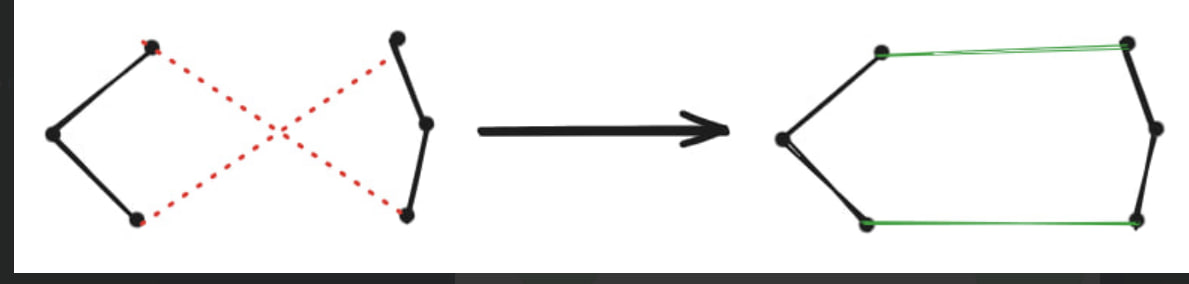
\includegraphics[width=0.78\textwidth]{fig_2opt_demo.png}
\caption*{Рисунок 4~--- Принцип 2-opt-перестановки. Слева~--- два маршрута с пересекающимися рёбрами (красный пунктир). Справа~--- после реверса сегмента между точками обмена новые рёбра (зелёные) короче, пересечение устранено, суммарная длина уменьшается.}
\label{fig:2opt-demo}
\end{figure}

Сам candidate-set строится поверх $k$-d~tree~[48]~--- структуры рекурсивного разбиения плоскости чередующимися осевыми гиперплоскостями: на каждом уровне точки делятся пополам по медиане одной координаты, на следующем~--- по другой. В получившемся дереве (рис.~5) запрос «найти $k$~ближайших соседей точки» обрабатывается за~$\Theta(\log n + k)$ амортизированно вместо $\Theta(n)$ при наивном переборе. Построение дерева~--- $\Theta(n\log n)$, выполняется один раз в начале работы решателя; все последующие 2-opt, repair и destroy-операторы пользуются предвычисленным candidate-set, что и даёт основное ускорение метаэвристики на крупных инстансах.

\begin{figure}[htbp]
\centering
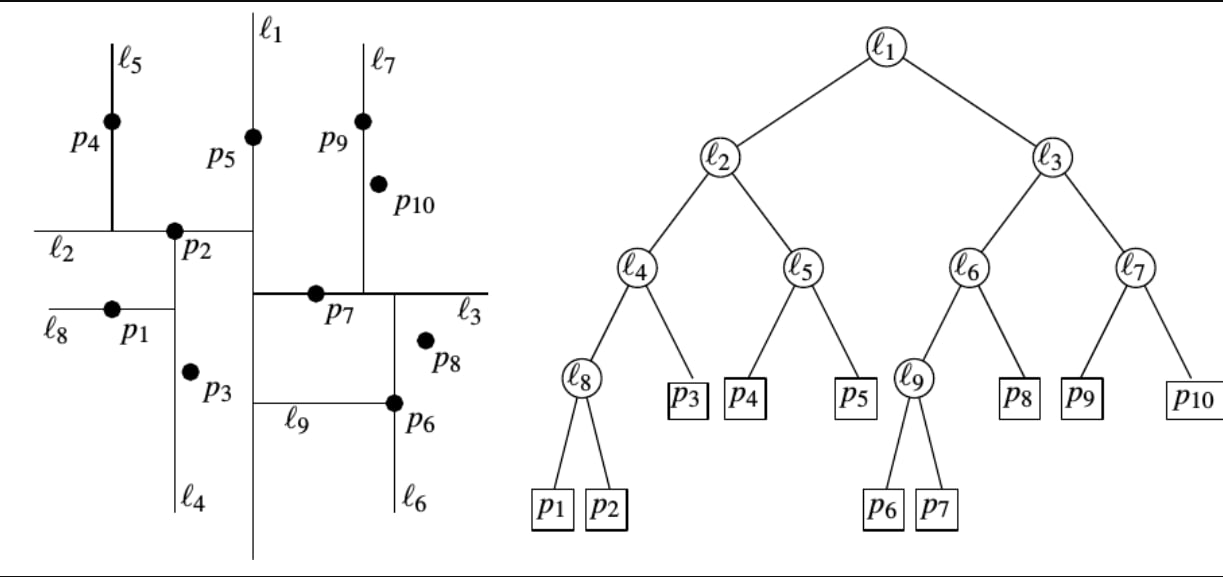
\includegraphics[width=0.88\textwidth]{fig_kdtree.png}
\caption*{Рисунок 5~--- $k$-d~tree на 10~точках. Слева~--- рекурсивное разбиение плоскости: на нечётных уровнях разделяющая прямая вертикальна (по~$x$), на чётных~--- горизонтальна (по~$y$); линии $\ell_1,\dots,\ell_9$ соответствуют узлам дерева. Справа~--- сам бинарный поиск-дерево: внутренние узлы хранят разделяющие прямые, листья~--- точки $p_1,\dots,p_{10}$. Запрос ближайшего соседа спускается по дереву за $\Theta(\log n)$, далее обходом смежных листов набирает $k$~ближайших.}
\label{fig:kdtree}
\end{figure}

\section{Прочие подходы и внешние ориентиры}
\label{sec:other-solvers}

\begin{figure}[htbp]
\centering
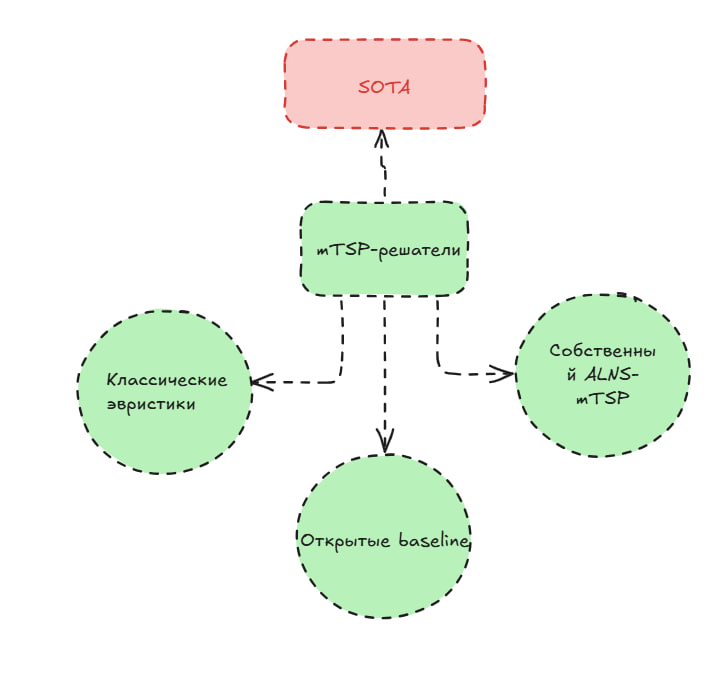
\includegraphics[width=0.55\textwidth]{fig_mtsp_solvers_taxonomy.png}
\caption*{Рисунок 6~--- Классификация решателей mTSP, рассматриваемых в работе. Три ветви~--- классические эвристики, открытые baseline-решатели и собственный ALNS-mTSP; отдельной категорией~--- специализированные SOTA-методы.}
\label{fig:mtsp-solvers-taxonomy}
\end{figure}

\textbf{Специализированные SOTA для min-max~mTSP} (HGA Mahmoudinazlou--Kwon~[35]; He--Hao MA~[29]; ITSHA; MILS) опубликованы только на $N\leq 1000$~--- применимость к~$N\geq 25\,000$ авторами не подтверждена. HGA и~He-Hao запущены на mTSPLib (см.~гл.~4); ITSHA и~MILS не запускались и учтены как направление дальнейшего сравнения.

\textbf{Нейросетевые SOTA} (Equity-Transformer, DPN, GLOP, DualOpt, UDC, H-TSP, DAN, iMTSP) не воспроизводились по трем причинам: (1)~специализированные mTSP-модели не публикуют результатов для~$N\geq 5\,000$, а универсальные TSP-модели не выполняют разбиение на~$m$~маршрутов; (2)~требуется переобучение при изменении $(n,m,$геометрия$)$; (3)~зависимость от GPU. Подробное описание~--- Приложение~З.

\textbf{Методологический базис.} Workload-equity-метрики~--- [28,33]; стандарты тестирования routing-методов~--- [34]; статистика~--- BCa-bootstrap~[38], Holm-коррекция~[39], Cliff's~$\delta$~[44], Cohen's~$d$~[45], FDR-контроль~[40], общие принципы bootstrap-методов~[46].

\textbf{Эталонные решатели и benchmark.} Помимо LKH-3 использовались FILO2~[6] (репозиторий~[51])~--- CVRP-решатель с~масштабированием до~$n\approx 10^6$, адаптируется на~mTSP через вместимость маршрута $Q=\lceil(n{-}1)/m\rceil$, и~OR-Tools~9.15~[5] (PATH\_CHEAPEST\_ARC + GUIDED\_LOCAL\_SEARCH). Стандартный benchmark min-max~mTSP~--- mTSPLib~[43]: 16~инстансов eil51, berlin52, eil76, rat99 с~$m\in\{2,3,5,7\}$.

\section{Собственный алгоритм ALNS-mTSP}

\textit{Позиционирование.} Точные методы неприменимы по~времени; LKH-3 default-MINSUM на~$N\geq 25K$ нарушает заявленный лимит и~даёт вырожденные решения, его балансирующие режимы дают 0/12 валидных за~30--60~мин; OR-Tools в~стандартной конфигурации не~справляется при~$N\geq 5K$; FILO2 в~CVRP-адаптации не~фиксирует ровно~$m$ маршрутов; специализированные min-max-метаэвристики опубликованы только на~$N\leq 1\,000$; воспроизведение нейросетевых SOTA требует GPU и~переобучения и~в~работе не~выполнено. Целевая ниша (mTSP с~$N$ до~100\,000, CPU без~GPU, лимит~$\sim$350\,c, ровно~$m$ нетривиальных маршрутов) в~рамках работы закрывается собственным ALNS-mTSP.

Собственный алгоритм ALNS-mTSP~--- итог эволюции линии \texttt{v1}\dots\texttt{v21} (см.~Приложение~Д) и~состоит из~четырёх специализированных решателей (\emph{alns\_minsum}, \emph{alns\_cap}, \emph{alns\_depot2m}, \emph{alns\_minmax}). Общая инфраструктура: KD-дерево, candidate-сеты, KNN, ALNS-каркас, операторы разрушения и~восстановления (Random, ClusterBfs, Expensive, Zone, Cheapest, Regret-2), направляемый локальный поиск (GLS), движок имитации отжига, пул параллельных стартов, автонастройка параметров, региональные granular-операторы~[22]. Подробное описание~--- глава~2 и~Приложение~А.

Общая схема работы решателя показана на~рисунке~7. На~вход подаются координаты $n$~клиентов и~число коммивояжеров~$m$. Начальное решение строится через кластеризацию $k$-means с~жадным алгоритмом Кларка--Райта; затем формируется список 10~ближайших соседей для каждого узла и~проводится локальный поиск 2-opt и~Or-opt внутри каждого маршрута. Основной адаптивный цикл чередует операторы разрушения (случайный, кластерный, удаление самых дорогих рёбер, удаление по~зоне) и~операторы восстановления (вставка по~минимальной стоимости, вставка с~приоритетом по~сожалению). Решения принимаются по~критерию Метрополиса с~экспоненциальным охлаждением; лучшее по~MINSUM решение запоминается в~архиве; веса операторов обновляются по~принципу рулетки. По~исчерпании бюджета времени запускается финальный 2-opt и~результат сериализуется в~JSON.

\begin{figure}[htbp]
\centering
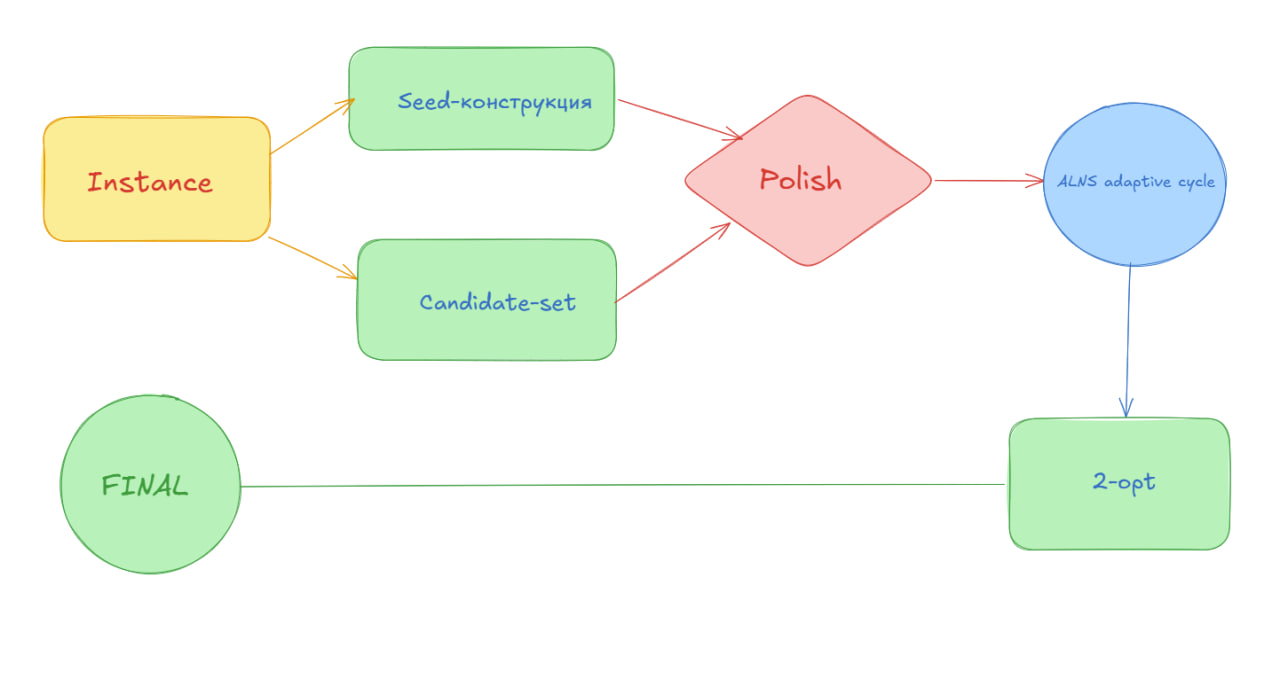
\includegraphics[width=\textwidth]{fig_alns_architecture.png}
\caption*{Рисунок~7~--- Общая схема ALNS-mTSP: seed-конструкция (k-means~+~Clarke--Wright savings) и построение candidate-сета (10-NN), внутримаршрутная полировка (2-opt~+~Or-opt), основной адаптивный цикл и финальный 2-opt по~исчерпании бюджета.}
\label{fig:alns-architecture}
\end{figure}

\begin{figure}[htbp]
\centering
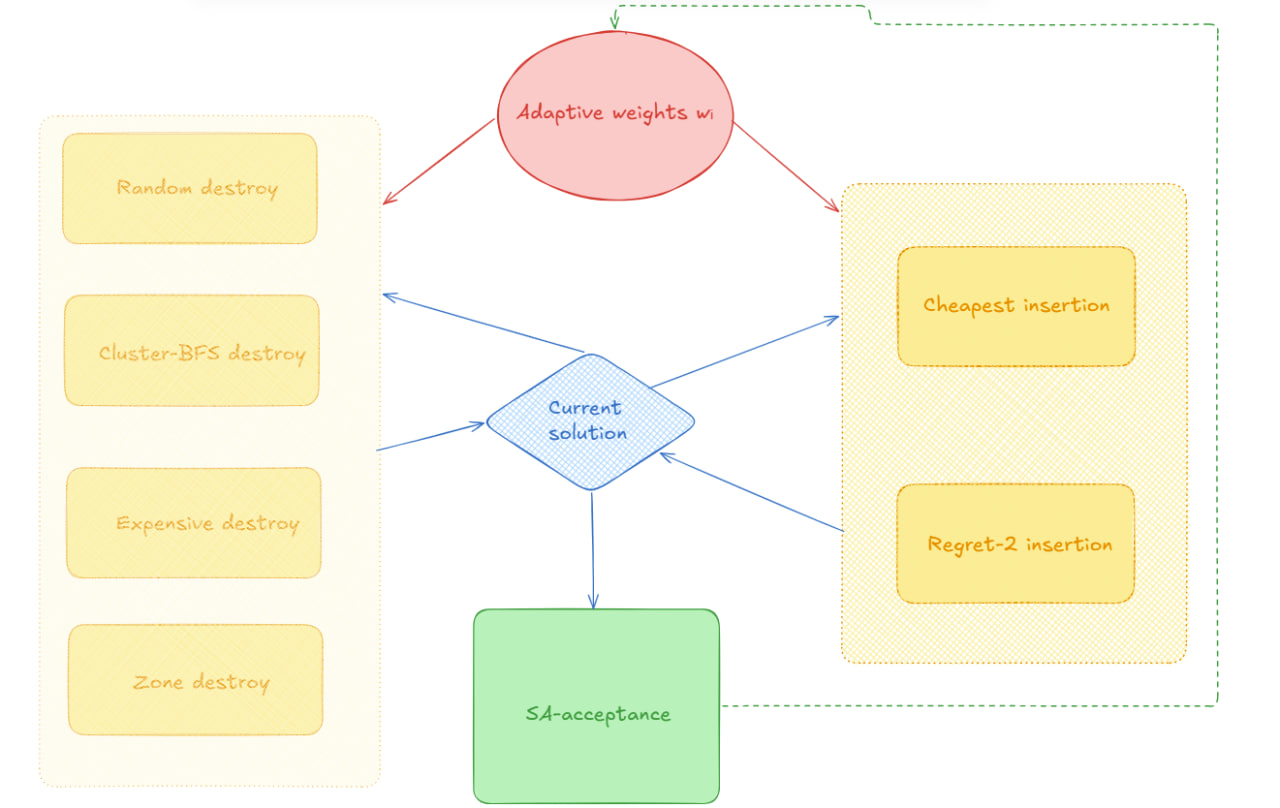
\includegraphics[width=\textwidth]{fig_alns_operator_cycle.png}
\caption*{Рисунок~8~--- Цикл destroy/repair с адаптивными весами: 4~destroy-оператора (Random, Cluster-BFS, Expensive, Zone) и 2~repair-оператора (Cheapest, Regret-2); выбор по~roulette-wheel, принятие хода~--- по~критерию Метрополиса (SA).}
\label{fig:alns-cycle}
\end{figure}

\medskip
Ключевая идея ALNS~--- \emph{ruin-and-recreate}: на каждой итерации destroy-оператор удаляет из~текущих маршрутов случайно выбранную долю клиентов (15--40\,\%), а repair-оператор пересчитывает оптимальную позицию для каждого из~них и вставляет обратно. Принятие хода управляется критерием Метрополиса с экспоненциально остывающей температурой. Веса операторов обновляются по принципу roulette wheel: оператор, давший улучшение, получает повышенный приоритет на~следующих итерациях. Иллюстрация типичной destroy/repair-итерации приведена на рисунке~9.

\begin{figure}[htbp]
\centering
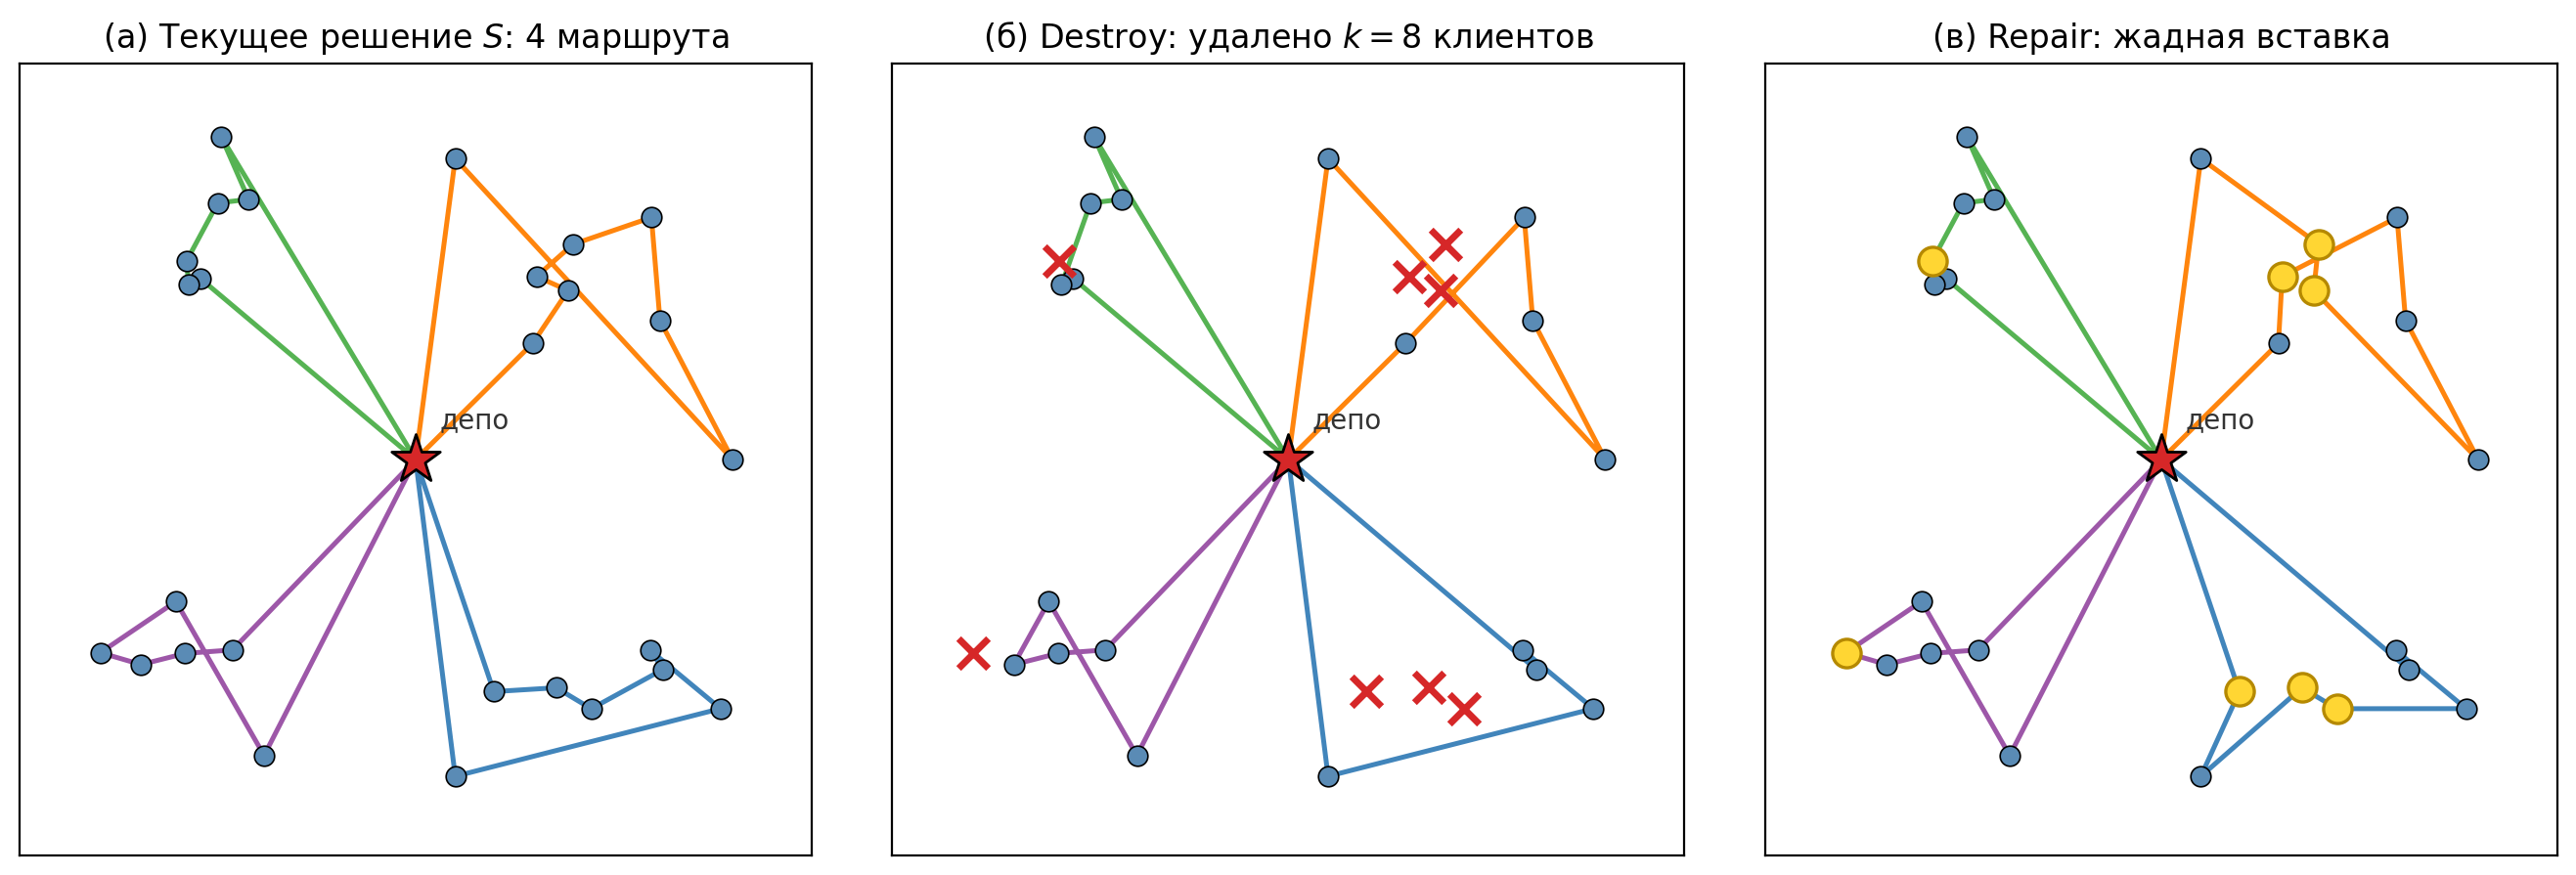
\includegraphics[width=0.85\textwidth]{fig_ruin_recreate_demo.png}
\caption*{Рисунок~9~--- Один цикл разрушения и~восстановления (ruin-and-recreate). \emph{(а)}: исходное решение из~4~маршрутов. \emph{(б)}: destroy-оператор удалил $k=8$ клиентов ($\approx 30\,\%$), маршруты перестроены в~обход удалённых точек. \emph{(в)}: repair-оператор (cheapest insertion) вставил клиентов обратно~--- часть оказалась в~других маршрутах, поэтому итоговая топология отличается от~(а).}
\label{fig:ruin-recreate-demo}
\end{figure}

\medskip
Внутри repair-фазы выбор между двумя базовыми стратегиями~--- \emph{cheapest insertion} и \emph{regret-2}~--- определяет, насколько repair устойчив к «жадным ловушкам». Cheapest insertion на каждом шаге вставляет того клиента, у которого минимальна абсолютная стоимость вставки $\Delta_{\min}$; regret-2 вместо этого сравнивает \emph{разрыв} $\mathrm{regret}=\Delta_{2nd}-\Delta_{1st}$ между лучшей и второй лучшей позицией и вставляет первым того клиента, у которого этот разрыв максимален. Идея: если у клиента есть только одна хорошая позиция (большой regret), его нужно вставить пока эта позиция доступна; если позиции примерно равноценны (малый regret), вставку можно отложить. На сложных инстансах эта разница дает regret-2 преимущество в~5--15\,\% по итоговому MINSUM (подтверждено ablation, разд.~4.5).
\begin{figure}[htbp]
\centering
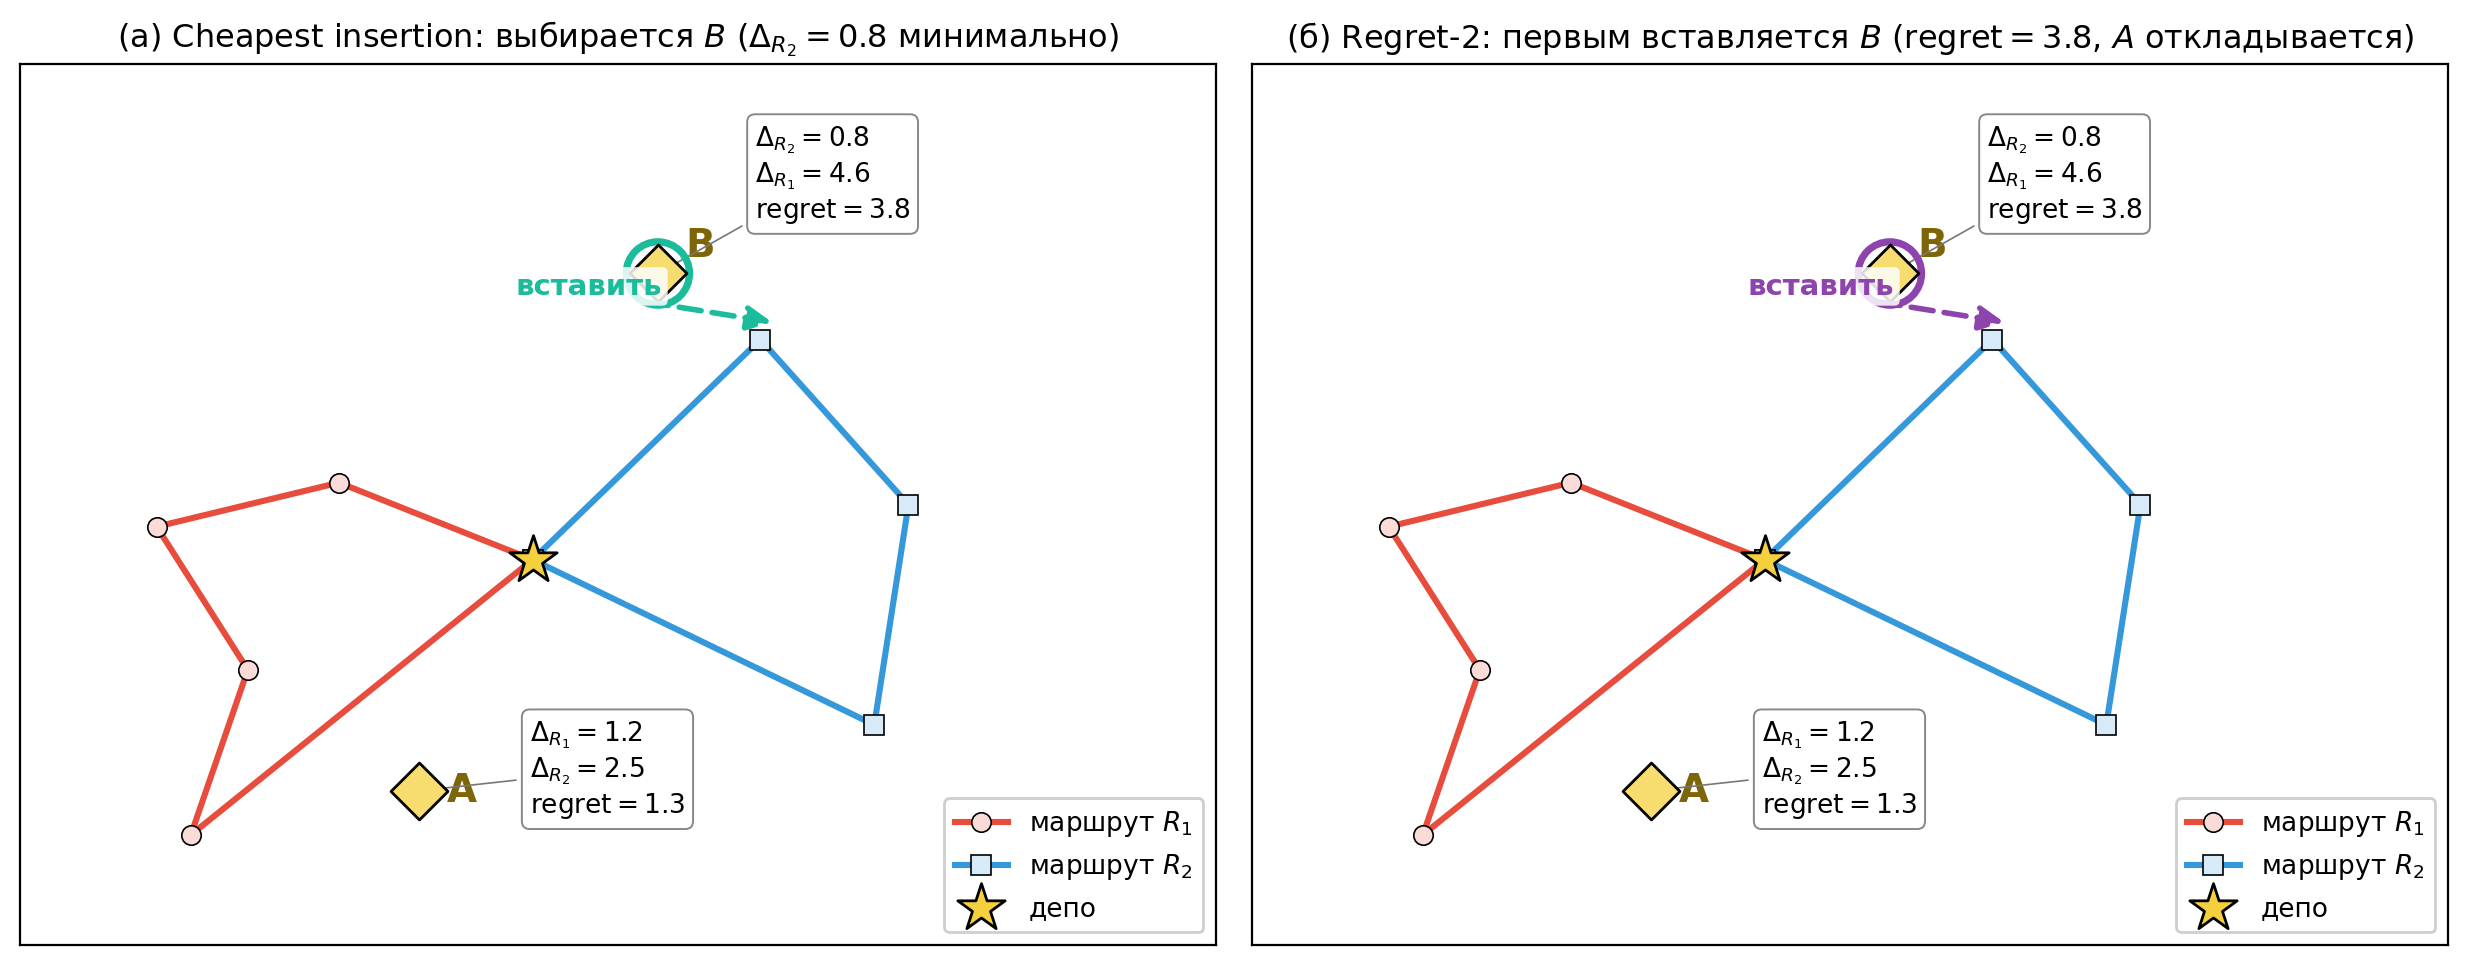
\includegraphics[width=0.96\textwidth]{fig_regret2_demo.png}
\caption*{Рисунок~9а~--- Cheapest insertion и~regret-2 на~одном сценарии. Два частичных маршрута $R_1,R_2$ и~два неназначенных клиента $A,B$; для каждого приведены стоимости вставки в~оба маршрута и~$\mathrm{regret}=\Delta_{2nd}-\Delta_{1st}$.}
\label{fig:regret2-demo}
\end{figure}

\noindent\textit{Чтение рисунка~9а.} Cheapest insertion (слева) выбирает~$B$, потому что~$\Delta_{R_2}=0.8$~--- минимальная абсолютная стоимость в~текущей конфигурации. Regret-2 (справа) тоже вставляет~$B$ первым, но~по~другой логике: у~$B$ $\mathrm{regret}=3.8$ (одна явно лучшая позиция, упустить которую дорого), у~$A$ $\mathrm{regret}=1.3$ (две сопоставимые позиции, вставку можно отложить). На~игрушечном сценарии порядок совпадает; на~реалистичном числе клиентов и~маршрутов стратегии расходятся и в~порядке вставок, и~в~итоговом качестве.

\section{Теоретическая оценка сложности}
\label{sec:complexity}

Поскольку TSP NP-трудна~[49] и~переносится на~mTSP по~сведению~[19,20], верхней границы полиномиального вида не~существует. Concorde на~$n>10\,000$ типично не~сходится в~разумное время, Held--Karp~[30] применим до~$n\approx 25$. LKH-3~--- метаэвристика без~полиномиальной верхней границы, доминирующая фаза~--- POPMUSIC~[25] ($\Theta(n^2/p\log n)$) и~$k$-opt-ход ($\Theta(k\cdot\mathrm{cand})$); эмпирическое время на~$N=25\,000$ в~9--12$\times$ превышает \texttt{TIME\_LIMIT} (табл.~5в). OR-Tools GLS использует $\Theta(n^2)$-первичную фазу, FILO2 дает $\Theta(n\log n)$ амортизированно. Для собственного ALNS-mTSP стоимость одной итерации~$\Theta(L+d\cdot k\cdot\log n)$, где $L=n/m$, $d$~--- размер destroy, $k$~--- размер candidate-сета. Эмпирический показатель степени~$\alpha=1.74$ (Прил.~Г.4) превышает теоретический линейный за счет потерь локальности кеша при операции реверса сегмента на длинных маршрутах. Полная декомпозиция и сводная таблица сложности~--- Приложение~Ж.

% =================================================================
% Глава 2
% =================================================================
\chapter{Сравнение архитектур исследуемых решателей}

В~этой главе кратко описаны архитектуры решателей, участвующих в~сравнении: эталонные LKH-3 и OR-Tools, классические эвристики и собственные модули семейства ALNS-mTSP. Особенности реализации, проявляющиеся на больших масштабах ($N \geq 25\,000$), определяют различия в~результатах. Теоретическая сложность~--- раздел~\ref{sec:complexity} и Приложение~Ж.

\section{LKH-3 в режиме MINSUM}

В основной сетке LKH-3 использовался в~чистом MINSUM-режиме с~\texttt{MTSP\_MIN\_SIZE\,=\,1}: базовая конфигурация без ограничения на минимальный размер маршрута, разрешающая $m{-}1$ маршрутам иметь длину 0~или~1. Это и~есть тот режим, в~котором default-LKH-3 на больших инстансах сваливается в~вырожденное решение (раздел~4.4, H1). Параметры запуска и~детали интеграции вынесены в~Приложение~Г.

Балансирующие режимы LKH-3 (\texttt{MIN\_SIZE\,=\,-1}, MINMAX) использовались только в~fair-baseline-сравнении на~малых инстансах (раздел~4.6) и~в~попытках масштабирования на~$N=25K$ (где не~уложились в~бюджет 30--60~мин,~--- раздел~4.2).

\section{ALNS-mTSP}

ALNS-mTSP~--- приоритетный объект работы. Четыре варианта (alns\_minsum, alns\_cap, alns\_depot2m, alns\_minmax) используют общий пайплайн \texttt{17\_pipeline.hpp} (фазы построения начального решения, candidate-сетов, ALNS-блока, полировки и финального 2-opt); различаются критерием приема (AcceptPolicy) и набором параметров по умолчанию.

\begin{itemize}
\item \emph{alns\_minsum}~--- стабильный базовый MINSUM-решатель; параметры подбираются автонастройкой (\texttt{18\_autotune.hpp}).
\item \emph{alns\_cap}~--- то же ядро с~ограничением максимального размера маршрута: $\mathrm{cap} = \lceil(n-1)/m\rceil \cdot (1+s)$, slack $s=0.75$ по умолчанию (идея заимствована из FILO2). Применяется при больших $m$ ($m \geq 50$).
\item \emph{alns\_depot2m}~--- экспериментальный преcет с фиксированной долей ALNS-фазы 86\,\%, использует семейство стартовых решений типа LKH-3 (один длинный маршрут + тривиальные) и встроенную пост-фазу перебалансировки 30\,000\,мс. Применяется когда приоритетна минимизация MINSUM ценой балансировки.
\item \emph{alns\_minmax}~--- MINMAX-вариант с критерием приема soft-$\alpha$ blend между $F_{\max}$ и~$F_{\mathrm{sum}}$.
\end{itemize}

Полное описание параметров и поведения каждого режима~--- Приложение~А.

\section{OR-Tools (Routing + GLS)}

Используется OR-Tools~9.15 в~стандартной конфигурации (\texttt{PATH\_CHEAPEST\_ARC + GUIDED\_LOCAL\_SEARCH}) с~переводом mTSP в~CVRP-формулировку: вместимость одного маршрута $Q=\lceil(n-1)/m\rceil$, запрос каждого клиента~$q_i=1$. На~малых инстансах ($N\leq 1000$)~--- конкурентоспособный решатель; на~$N\geq 5\,000$ в~использованной конфигурации не~уложился в~заданный бюджет с~практически приемлемым решением (см.~главу~4).

\section{Классические эвристики}

\emph{rand+nn} (рандомизированный round-robin nearest-neighbor) и \emph{2opt+greed} (round-robin nearest-neighbor + жадный 2-opt до сходимости) служат нижней границей Парето-кривой качество--время. На~$N=100\,000$ время работы \emph{2opt+greed} достигает 137--257\,c.

% =================================================================
% Глава 3
% =================================================================
\chapter{Описание экспериментальной программы}

В~главе описаны: подготовка набора инстансов, главная программа сравнения, метрики качества и времени, особенности запуска отдельных решателей, стратегия стратифицированного бенчмарка и сводная таблица всех экспериментов.

\section{Подготовка набора инстанций}

Для контроля воспроизводимости использован собственный генератор синтетических инстансов, поддерживающий шесть геометрических семейств: uniform (равномерное распределение клиентов), clustered-center (несколько компактных кластеров около центра поля), clustered-offset-depot (то~же, но депо смещено к~границе поля), mixed-outliers (кластеры с~долей outlier-клиентов), outliers (плотное ядро~+ далёкие точки), high-m (геометрия для тестирования при больших~$m$). Координаты генерируются на~квадрате $100\times 100$ с~фиксированным base-seed; формат~--- текстовый, первая строка \texttt{n m}, далее $n$ строк с~координатами \texttt{x y}, вершина~0~--- депо.

Использованы два набора инстансов:
\begin{itemize}\itemsep1pt
\item \textbf{Малый страт:} 60~инстансов c~$N\in\{100,\,200,\,500,\,1000\}$, $m\in\{3,5,7\}$, 3~повтора на~каждую тройку $(n,m,\text{family})$;
\item \textbf{Большой страт (мультисемейный):} 215~инстансов c~$N\in\{5000,\,10\,000,\,25\,000,\,50\,000,\,100\,000\}$, $m\in\{3,5,7,10,30,50,80,100\}$ в~зависимости от~$N$, по~1~повтору на~$(n,m,\text{family})$.
\end{itemize}

Скрипт-генератор и~пути к~артефактам~--- Приложение~В.

\section{Главная программа сравнения}

Главная программа сравнения принимает на~вход JSON-конфигурацию со~списком решателей и~набором фильтров (\texttt{allowed\_node\_counts}, \texttt{allowed\_salesman\_counts}, \texttt{instance\_families}). Для каждой пары $(\text{instance},\text{solver})$ вызывается общий C++-binary с~указанным бюджетом времени и~парсится JSON-вывод (целевая функция, время, валидность, маршруты, внутренние счётчики решателя); результаты сохраняются в~per-run и~агрегатном CSV по~$(\text{family},n,m,\text{solver})$.

Главная программа доработана так, что~при сбое одиночного запуска (нестандартный возврат WSL-процесса, превышение лимита памяти, несвоевременный выход решателя) общий прогон не~прерывается~--- фиксируется строка с~\texttt{valid=False} и~статусом \texttt{crashed:<message>}. Это было критично при работе с~\emph{lkh3-baseline-minmax}, периодически нарушающим \texttt{TIME\_LIMIT} в~десятки раз. Скрипт и~артефакты~--- Приложение~В.

\section{Метрики качества и времени}

\textbf{Качество решения.} Помимо целевых функций~(\ref{eq:minsum}) и~(\ref{eq:minmax}) фиксируется число тривиальных маршрутов~--- $n_\mathrm{empty}$ маршрутов вида $(0,0)$ и $n_\mathrm{singl}$ маршрутов вида $(0,c,0)$.

\textbf{Метрики баланса маршрутов.} Пусть $\overline{\mathrm{len}}=F_{\mathrm{sum}}(R)/m$~--- средняя длина маршрута. В~работе используются две взаимодополняющие метрики из~обзора workload-equity~[28]:
\begin{align}
\mathrm{Gini}(R) &= \frac{1}{2m^2\,\overline{\mathrm{len}}}\sum_{i=1}^{m}\sum_{j=1}^{m}\bigl|\mathrm{len}(R_i)-\mathrm{len}(R_j)\bigr|,\qquad \mathrm{Gini}(R)\in\bigl[0,\,1-\tfrac{1}{m}\bigr],\label{eq:gini}\\
\mathrm{bal}(R) &= \frac{F_{\max}(R)}{\overline{\mathrm{len}}}\;=\;m\cdot\frac{F_{\max}(R)}{F_{\mathrm{sum}}(R)},\qquad \mathrm{bal}(R)\in[1,\,m].\label{eq:bal}
\end{align}
Идеально сбалансированное решение даёт $\mathrm{Gini}=0$, $\mathrm{bal}=1$; вырожденное (один маршрут несёт всех клиентов)~--- $\mathrm{Gini}\to 1-1/m$, $\mathrm{bal}\to m$. Гини~--- стандартизованная в литературе оценка неравенства, учитывающая весь профиль длин; $\mathrm{bal}$~--- интуитивный коэффициент дисбаланса, основанный только на экстремуме. Дополнительные стандартные метрики (range, MAD, std) вычисляются в \texttt{compute\_review\_metrics.py}, но в сравнительных таблицах не приводятся~--- $\mathrm{Gini}$ и $\mathrm{bal}$ качественно эквивалентно разделяют сбалансированный и вырожденный классы решений.

\textbf{Метрика относительного отрыва.} Для парных сравнений двух решателей~$A$ и~$B$ на одинаковой инстанции~$I$ используется относительная разность по MINSUM:
\begin{equation}
\Delta_{A,B}(I)\;=\;\frac{F_{\mathrm{sum}}^{A}(I)-F_{\mathrm{sum}}^{B}(I)}{F_{\mathrm{sum}}^{B}(I)}\cdot 100\,\%,
\label{eq:delta}
\end{equation}
где $B$~--- baseline. Отрицательное $\Delta_{A,B}$ означает, что~$A$ лучше~$B$ по MINSUM на данной инстанции.

\textbf{Wall-clock и валидность.} Время работы измерялось Python-оберткой; валидность контролируется независимым пересчётом~(\ref{eq:route-length}) по сохранённым маршрутам и проверкой условий (а)--(в) Определения~1.

\medskip
\textbf{Constraint-first протокол сравнения.} Во всех сравнениях, относящихся к практическому сценарию работы, MINSUM сопоставляется только среди решений, удовлетворяющих трём ограничениям одновременно:
\begin{enumerate}\itemsep1pt
\item \textbf{(i)} время работы $t\leq T_\mathrm{budget}$ (бюджет соответствующего стратума: 10--30\,c, 150\,c или 250--350\,c);
\item \textbf{(ii)} ровно $m$ нетривиальных маршрутов ($n_r=m$, $n_\mathrm{empty}=n_\mathrm{singl}=0$);
\item \textbf{(iii)} приемлемая балансировка ($\mathrm{Gini}\leq 0.05$ или $\mathrm{balance\_max\_avg}\leq 1.10$ на больших инстансах; $\mathrm{balance}\leq 1.5$ на малых).
\end{enumerate}
Решения, нарушающие хотя бы одно из условий~(i)--(iii), исключаются из количественного сравнения по~MINSUM~--- меньшая сумма при~$n_r\neq m$ или~$\mathrm{Gini}\to 1{-}1/m$ не~индексирует более качественное решение в~постановке работы (пример: $[24993,3,1,1,1]$ у~LKH-3 default). Constraint-first протокол применяется сквозным образом: в~формулировке гипотез работы (введение), в~архитектурном позиционировании ALNS-mTSP (раздел~1.4), во~всех количественных таблицах главы~4 и~в~итоговой сводке прохождения практического фильтра (раздел~4.9 «Статус гипотез работы»). Этот протокол~--- центральная методологическая позиция работы: вырожденные решения по~MINSUM (LKH-3 default, alns\_depot2m) могут давать формально меньшую сумму, но~\emph{не считаются приемлемыми} в~смысле постановки работы, поскольку выходят за~рамки практического фильтра.

\textbf{Статистические инструменты.} Парные сравнения~--- Wilcoxon signed-rank (\texttt{scipy.stats.wilcoxon}); CI~--- 95\,\% percentile/BCa-bootstrap (10\,000~ресэмплов, \texttt{scipy.stats.bootstrap}); эффект~--- Cliff's~$\delta$; контроль FWER на семействах сравнений~--- Holm-коррекция.

\section{Особенности работы исследуемых решателей}

В ходе экспериментов были выявлены следующие нетривиальные особенности.

LKH-3 в режиме MINMAX (\texttt{MTSP\_OBJECTIVE = MINMAX}) на больших инстанциях не соблюдает заданный лимит времени (\texttt{TIME\_LIMIT}): на $N = 1000$, $m = 5$ при лимите 30~секунд решатель тратит до~668 секунд, на $N = 25\,000$~--- до~1\,600 секунд при лимите 150~секунд, на $N = 50\,000$~--- оценочно более часа. Это связано с внутренней логикой обработки penalties: одна итерация 5-opt может занимать минуты на больших candidate-сетах. По этой причине из ряда конфигураций экспериментов LKH-3 в MINMAX-режиме был исключен.

Решатель \emph{alns\_depot2m} имеет встроенную пост-фазу перебалансировки длительностью \texttt{rebalance\_post\_ms = 30\,000~мс} по умолчанию; эта фаза не входит в основной лимит \texttt{time-budget-ms}, что означает, что фактическое время работы превышает заданный лимит на величину пост-фазы.

OR-Tools на инстанциях $N \geq 5000$ в стандартной конфигурации \texttt{PATH\_CHEAPEST\_ARC + GUIDED\_LOCAL\_SEARCH} при лимите 70~секунд возвращает решение на 1--2 порядка худшее по MINSUM, чем ALNS-mTSP-семейство.

\section{Стратегия стратифицированного бенчмарка}

Сетка экспериментов организована послойно:
\begin{itemize}\itemsep1pt
\item \emph{малые инстансы} ($N\leq 1000$, бюджет 10--30~с)~--- полное покрытие 60~инстансов на~10~конфигурациях решателей, основной материал раздела~4.1;
\item \emph{слой верификации} ($N=25\,000$, бюджет 150~с)~--- 5~решателей с~самостоятельно собранным binary LKH-3, основной материал раздела~4.2;
\item \emph{большие данные} ($N\in\{50\,000,\,100\,000\}$, бюджет 250--350~с)~--- основная сетка ALNS-mTSP-семейства плюс прямое сравнение с~FILO2 на~12~ячейках (раздел~4.7); LKH-3 на~этом масштабе исключён из-за многочасового времени работы (раздел~4.2, табл.~5в).
\end{itemize}

\noindent\textbf{Промежуточный слой $N\in\{5\,000,\,10\,000\}$.} Между малым и~верификационным слоями проведены точечные эксперименты на~промежуточных~$N$:
\begin{itemize}\itemsep1pt
\item OR-Tools на~$N=5\,000$ при~лимите 70~с~--- проверка гипотезы~H4 о~непригодности стандартной конфигурации на~$N\geq 5K$ (раздел~4.4);
\item high-m sweep на~$N=10\,000$ для $m\in\{10,\dots,100\}$, 15~ячеек~--- проверка гипотезы~H5 о~росте преимущества с~$m$ (раздел~4.4);
\item CLI-ablation \emph{alns\_minsum} на~$N=10\,000$ (4~варианта~$\times$~3~seeds)~--- раздел~4.5, табл.~7а.
\end{itemize}
Эти запуски не~образуют полноценный страт (нет систематического покрытия всех семейств и~всех решателей), но~закрывают конкретные методологические вопросы и~поэтому проходят отдельно от~трёх основных слоёв.

\section{Сводка экспериментальной программы}
\label{sec:experiment-summary}

Сводка ключевых экспериментов работы~--- таблица~3.1.

\medskip
\noindent Таблица 3.1~--- Ключевые эксперименты ($\geq 2\,157$ валидных запусков).

\begin{center}\small
\begin{tabular}{|L{3.0cm}|C{1.0cm}|L{3.5cm}|L{5.0cm}|}
\hline
\textbf{Эксперимент} & \textbf{Раздел} & \textbf{Объём} & \textbf{Главный результат} \\
\hline
Малые инстансы & 4.1 & 60~инст.~$\times$~3~повт.~$\times$~10~конфиг. & alns\_minsum vs LKH-3 default: $\Delta=-3.48\,\%$ ($p=0.046$) \\
\hline
N=25K (верификация) & 4.2 & 4~ячейки $\times$ 5~решат. + 22~LKH-3 long-budget & LKH-3 в~9--12$\times$ нарушает TIME\_LIMIT; balanced-режимы 0/12 валидных \\
\hline
N=25K, 50K, 100K & 4.2--4.3 & 18~ячеек $\times$ 5~seeds = 90~runs & alns\_minsum: Gini~$\leq 0.05$, max-route в~$4{-}6\times$ меньше depot2m+ \\
\hline
Fair-baseline LKH-3 & 4.6 & 48~инст. $\times$ 3~режима = 144 & ALNS vs balanced LKH-3: $-13\dots-18\,\%$ ($p<10^{-13}$) \\
\hline
FILO2 на больших инстансах & 4.7 & 18~ячеек~+~прямое сравнение $N=100K$ & 2/18~валидных; FILO2 нарушает~$m_\mathrm{target}$ \\
\hline
HGA / He-Hao на mTSPLib & 4.8 & 16~ячеек $\times$ 2~SOTA + multi-seed & HGA доминирует по~makespan на mTSPLib, не масштабируется $N\geq 25K$ \\
\hline
Ablation & 4.5 & 4~варианта $\times$ 3~ключевых $\times$ 3~seeds & classic-seeds~--- доминирующий компонент ($+8.6\,\%$ при~отключении) \\
\hline
\end{tabular}
\end{center}

\medskip
Главный количественный аргумент работы~--- триангуляция: (а)~fair-baseline LKH-3 на малых инстансах усиливает преимущество ALNS-mTSP; (б)~workload-equity на больших инстансах с bootstrap-CI~$\leq 1\,\%$; (в)~непригодность LKH-3 в balanced-режимах на $N\geq 25K$; (г)~непригодность FILO2 в CVRP-адаптации.

% =================================================================
% Глава 4
% =================================================================
\chapter{Результаты и проверка гипотез}

В~главе представлены количественные результаты по~стратифицированной сетке трёх масштабов: \emph{малые инстансы} ($N\leq 1K$, раздел~4.1), \emph{слой верификации} ($N=25K$, раздел~4.2), \emph{большие инстансы} ($N\in\{50K,\,100K\}$, раздел~4.3); дополнительно~--- точечные эксперименты на~промежуточном слое $N\in\{5K,\,10K\}$ (high-m sweep, OR-Tools~H4, CLI-ablation~--- в~рамках разделов~4.4 и~4.5). Проверены гипотезы~H1--H6, проведён ablation, fair-baseline-сравнение с~LKH-3 в~балансирующем режиме и~сравнение с~внешними решателями (mTSPLib, FILO2, длительный прогон LKH-3). Глава завершается проверкой главной гипотезы.

\section{Малые инстансы ($N = 100\dots1000$)}

На стратифицированном прогоне $N = 100\dots1000$ (60~инстансов, 3~повтора на каждую $(n, m,$~family$)$) проверены десять конфигураций решателей: rand+nn, 2opt+greed, ortools-GLS, lkh3-baseline (MINSUM), lkh3-baseline-minmax, lkh-wrapper-v21, alns\_minsum, alns\_cap, alns\_depot2m, alns\_minmax.

Главные наблюдения. На~$N=100{-}200$ \emph{alns\_minsum} лидирует по~MINSUM в~11/12~ячеек (на~clustered с~большим~$m$ превосходит LKH-3 на~12--22\,\%). На~$N=500{-}1000$ LKH-3 опережает в~7/8~ячеек на~1--3\,\%, но дает вырожденные решения вида~$[995,1,1,1,1]$. \texttt{balance\_max\_avg}: у~LKH-3 default~$\approx 5.0/7.0$ (для~$m=5/7$), у ALNS-mTSP~$\approx 1.0{-}1.1$.

\medskip
\noindent Таблица 1а~--- Парные сравнения ALNS-вариантов с~LKH-3 default-MINSUM на 60~общих $(N, m,$family$,$repeat$)$-малых инстансах: средняя относительная разница, 95\,\% \emph{BCa-bootstrap-CI} (DiCiccio~\& Efron 1996), Wilcoxon signed-rank $p$-value (двухсторонний), Holm-скорректированный $p$ (FWER на~семействе из 4-х сравнений) и Cliff's~$\delta$ effect~size. Положительное значение средней разности означает, что соответствующий ALNS-вариант хуже LKH-3 (больше MINSUM); отрицательное~--- лучше.

\begin{center}\footnotesize
\begin{tabular}{|L{3.0cm}|C{0.7cm}|C{1.4cm}|C{2.4cm}|C{1.5cm}|C{1.5cm}|C{1.6cm}|}
\hline
\textbf{ALNS-вариант} & $N$ & \textbf{$\overline{\Delta_{\mathrm{rel}}}$,\,\%} & \textbf{95\,\% BCa CI} & \textbf{Wilcoxon $p$} & \textbf{Holm $p_{\mathrm{adj}}$} & \textbf{Cliff $\delta$} \\
\hline
\emph{alns\_minsum}              & 60 & $-3.48$ & $[-5.32,\,-1.98]$ & $0.046$ & $0.138$ & $-0.30$ (small) \\
\hline
\emph{alns\_cap}                 & 60 & $-1.00$ & $[-2.94,\,+0.45]$ & $0.160$ & $0.319$ & $\approx 0$ (negligible) \\
\hline
\emph{alns\_depot2m}             & 60 & $+1.18$ & $[+0.91,\,+1.51]$ & $9.9{\cdot}10^{-11}$\,$^{*}$ & $4.0{\cdot}10^{-10}$\,$^{*}$ & $+0.93$ (large, противоп. знак) \\
\hline
\emph{lkh-wrapper-v21}           & 60 & $-0.36$ & $[-2.75,\,+1.91]$ & $0.219$ & $0.319$ & $\approx 0$ (negligible) \\
\hline
\multicolumn{7}{|p{14cm}|}{\footnotesize $^{*}$~--- значимо при~$\alpha=0.05$ \emph{после Holm--Bonferroni-коррекции} на~семействе из~4~сравнений.}\\
\hline
\end{tabular}
\end{center}

\medskip
\noindent\textit{Методические пояснения к~табл.~1а.} Доверительный интервал для среднего относительного отклонения рассчитан BCa-бутстрепом (10\,000 ресэмплов, фиксированный seed для воспроизводимости): этот вариант бутстрепа корректнее обычного percentile-метода на~асимметричных распределениях разностей~--- а здесь как~раз наблюдается левосторонняя скошенность $g_1\in[-1.25,\,-0.60]$. Величина эффекта Cliff's~$\delta$ интерпретируется по~стандартной шкале: $|\delta|<0.147$~--- эффект пренебрежимо мал; $0.147\dots 0.33$~--- малый; $0.33\dots 0.474$~--- средний; $|\delta|\geq 0.474$~--- большой. Скрипт расчёта и~артефакты~--- Приложение~В.

\textit{Интерпретация.} Средний выигрыш \emph{alns\_minsum} над LKH-3 default $-3.48 \pm 1.7\,\%$ (95\,\% CI~$\not\ni 0$, Wilcoxon~$p=0.046$), но после Holm-коррекции $p_{\mathrm{adj}}=0.138$ — \emph{не выживает} FWER при~$\alpha=0.05$, Cliff's~$\delta=-0.30$ (small). \emph{depot2m} систематически проигрывает (${+}1.18\pm 0.30\,\%$, $p_{\mathrm{adj}}=4.0\cdot 10^{-10}$, $\delta=+0.93$, large). \emph{alns\_cap}, \emph{lkh-wrapper-v21}~--- статистически неотличимы. В разделе~4.6 (табл.~4б) приведён более чистый fair-baseline с балансирующими режимами LKH-3; там разрыв возрастает до~$13{-}18\,\%$, однако часть этого разрыва объясняется тем, что balanced-LKH-3 ограничен через \texttt{MIN\_SIZE/MAX\_SIZE}, тогда как ALNS-mTSP на малых $N\leq 500$ может сам выбирать вырожденную конфигурацию (см.~оговорку в~разделе~4.6).

\textit{Симметрия Wilcoxon.} Парные разности имеют отрицательную скошенность ($g_1\in[-1.25, -0.60]$); Shapiro--Wilk отвергает нормальность ($p<0.02$). Умеренное нарушение симметричной альтернативы; большие effect~sizes делают вывод устойчивым (см.~ограничение~7).

\section{Слой верификации ($N = 25\,000$)}

\noindent Таблица~2~--- $N=25\,000$, uniform, $m\in\{5,7\}$ (single-seed; 5-seed mean для ALNS-вариантов см.~табл.~5б). \emph{bal}~=~$\mathrm{balance\_max\_avg}$, \emph{makesp}~=~$F_{\max}/10^3$.

\begin{center}\small
\begin{tabular}{|C{0.4cm}|L{4.0cm}|R{1.5cm}|R{1.2cm}|C{1.1cm}|R{1.1cm}|C{1.2cm}|}
\hline
$m$ & \textbf{Решатель} & \textbf{sum} & \textbf{makesp} & \textbf{Gini} & \textbf{bal} & \textbf{$t$,\,c} \\
\hline
5 & lkh3-baseline & 1\,419\,561 & 1\,419 & 0.800 & 5.00 & 1\,608 \\ \hline
5 & alns\_depot2m & 1\,569\,641 & 1\,569 & 0.800 & 5.00 & 193 \\ \hline
5 & alns\_minsum  & 1\,592\,819 & 346 & 0.028 & 1.09 & 89 \\ \hline
5 & alns\_cap     & 1\,602\,522 & 343 & 0.022 & 1.07 & 90 \\ \hline
5 & lkh-wrapper-v21 & 1\,671\,488 & 356 & 0.020 & 1.06 & 152 \\ \hline
\hline
7 & lkh3-baseline & 1\,419\,836 & 1\,419 & 0.857 & 7.00 & 1\,643 \\ \hline
7 & alns\_depot2m & 1\,610\,580 & 832 & 0.719 & 3.62 & 195 \\ \hline
7 & alns\_minsum  & 1\,659\,764 & 261 & 0.047 & 1.10 & 92 \\ \hline
7 & alns\_cap     & 1\,669\,763 & 262 & 0.050 & 1.10 & 91 \\ \hline
7 & lkh-wrapper-v21 & 1\,789\,729 & 278 & 0.036 & 1.09 & 150 \\ \hline
\end{tabular}
\end{center}

\medskip
\textit{Главные наблюдения.} LKH-3 даёт лучший MINSUM, но ценой вырождения: 24\,993 клиента в одном маршруте (Gini~$\to 1{-}1/m$). Время LKH-3~--- 1\,608/1\,643\,c, в~10$\times$ превышает TIME\_LIMIT=150\,c (POPMUSIC-фаза не подчиняется лимиту). \emph{alns\_depot2m} воспроизводит default-MINSUM-стратегию LKH-3 в практическом бюджете 193\,c. \emph{alns\_minsum/cap} дают балансированное решение (Gini~$\leq 0.05$) за 89--91\,c; max-route на~$m=5$ в~$4.1\times$ меньше LKH-3.

\medskip
\textit{Дополнительный длительный прогон LKH-3.} При лимите 1\,800--3\,600\,c из 22~попыток (3~режима LKH-3) \textbf{5 завершились} в~default-MINSUM-режиме (Gini~$\in[0.40,0.86]$, $\Delta\mathrm{MINSUM}=-12\dots-20\,\%$ к ALNS), все 12~balanced-режимов~--- 0/12 валидных за 30--60~минут. Артефакт: \texttt{lkh3\_large\_n\_results.csv}.

\begin{figure}[ht]
\centering
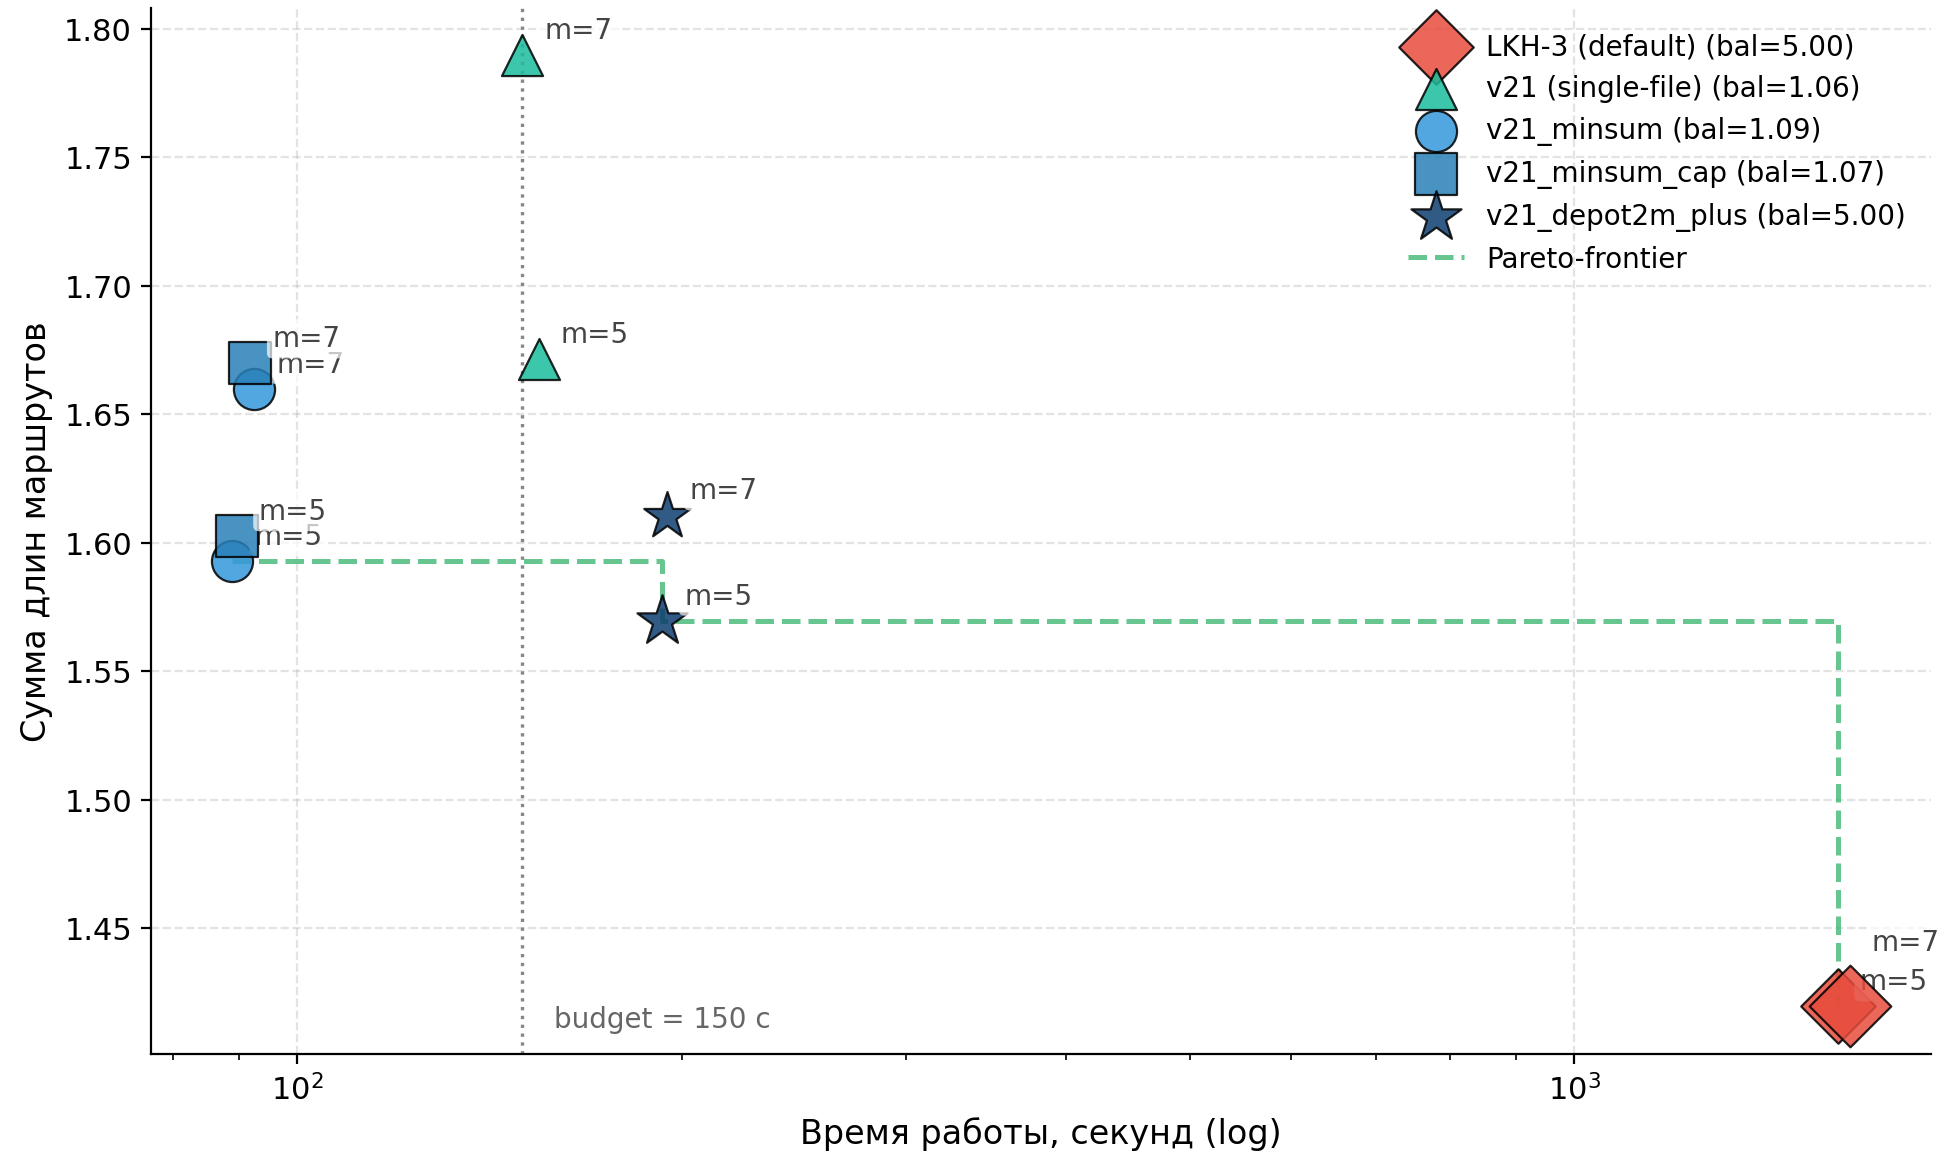
\includegraphics[width=0.85\textwidth]{fig6_pareto_dominance_n25k.png}
\caption*{Рисунок 10~--- Pareto-доминирование на $N = 25\,000$ (uniform): размер маркера пропорционален \texttt{balance\_max\_avg}. На Pareto-frontier~--- alns\_minsum (быстро, средний SUM, bal~$\approx$~1.09) и LKH-3 default (медленно, лучший SUM, bal~=~5.0). Вертикальный пунктир~--- заданный лимит времени 150~с, LKH-3 нарушает его в~10$\times$.}
\end{figure}

\section{Большие данные ($N = 50\,000$ и $N = 100\,000$)}

Стратум-3 разбит на два подэксперимента: $N=50K$ (4~ALNS-решателя, LKH-3 исключён~--- оценочное время $>50$~мин/инст.) и $N=100K$ (4~ALNS + \emph{2opt+greed}, LKH-3 $>8$\,ч/инст.). 6~ячеек~$\times$~семейства~$\{$uniform, clust-center, clust-offset$\}$~$\times$~$m\in\{5,7\}$.

\medskip
\noindent Таблица 4~--- Результаты на $N\in\{50K,100K\}$, uniform (single-seed; 5-seed mean см.~табл.~5б). \emph{bal}~=~balance\_max\_avg.

\begin{center}\small
\setlength{\tabcolsep}{5pt}
\begin{tabular}{|C{1.0cm}|C{0.5cm}|L{2.6cm}|R{1.7cm}|R{1.5cm}|C{0.9cm}|C{1.0cm}|}
\hline
$N$ & $m$ & \textbf{Решатель} & \textbf{sum} & \textbf{max-route} & \textbf{bal} & \textbf{$t$,\,c} \\
\hline
50K  & 5 & \emph{alns\_cap}       & 4\,512\,978 & 949\,k    & 1.03 & 163 \\ \hline
50K  & 5 & \emph{alns\_minsum}    & 4\,526\,397 & 950\,k    & 1.05 & 161 \\ \hline
50K  & 5 & \emph{alns\_depot2m}   & 4\,615\,081 & 4\,615\,k & 5.00 & 292 \\ \hline
50K  & 7 & \emph{alns\_cap}       & 4\,828\,936 & 690\,k    & 1.05 & 157 \\ \hline
50K  & 7 & \emph{alns\_minsum}    & 4\,834\,299 & 690\,k    & 1.05 & 155 \\ \hline
50K  & 7 & \emph{alns\_depot2m}   & 4\,765\,698 & 2\,313\,k & 3.40 & 284 \\ \hline
\hline
100K & 5 & \emph{alns\_depot2m}   & 12\,149\,667 & 12\,148\,k & 5.00 & 409 \\ \hline
100K & 5 & \emph{alns\_minsum}    & 12\,993\,166 & 2\,655\,k  & 1.02 & 345 \\ \hline
100K & 5 & \emph{alns\_cap}       & 13\,022\,451 & 2\,688\,k  & 1.03 & 345 \\ \hline
100K & 7 & \emph{alns\_depot2m}   & 12\,137\,649 & 12\,135\,k & 7.00 & 433 \\ \hline
100K & 7 & \emph{alns\_minsum}    & 13\,055\,628 & 1\,999\,k  & 1.07 & 344 \\ \hline
100K & 7 & \emph{alns\_cap}       & 13\,077\,285 & 1\,996\,k  & 1.07 & 344 \\ \hline
\end{tabular}
\end{center}

\noindent\textit{Clustered-семейства ($N=100K$).} На~clust-center \emph{alns\_minsum} даёт max-route в~$1.5\times$ меньше \emph{alns\_depot2m} при~$\Delta\mathrm{sum}=+5\,\%$; на~clust-offset~--- max-route в~$4.2\times$ меньше при~$\Delta\mathrm{sum}=+13\,\%$ для~$m=5$ и~в~$6.1\times$ меньше при~$\Delta=+11\,\%$ для~$m=7$. Артефакт~--- Приложение~В.

\medskip
\textit{Главное наблюдение.} \emph{depot2m+} даёт лучший формальный MINSUM на 6/6~ячейках $N=100K$ (на 5--12\,\% меньше \emph{minsum/cap}) ценой полного вырождения: на uniform/clust-offset одна TSP-петля через 99\,995--99\,999 точек ($\mathrm{Gini}\in[0.80,0.86]$). Сбалансированные \emph{alns\_minsum/cap} держат $\mathrm{Gini}\leq 0.022$ при~$\Delta\mathrm{sum}=+5\dots+13\,\%$~--- основной практический компромисс.

\medskip
\noindent Таблица 5б~--- Multi-seed variance audit \emph{alns\_minsum} на всех 18 ячейках стратума-3 (3 семейства $\times$ 3 размера $\times$ 2 значения~$m$, \textbf{5 независимых seed} на ячейку, итого~90 валидных запусков). cv $\in [0.04\%, 0.71\%]$.

\begin{center}\footnotesize
\begin{tabular}{|L{2.4cm}|C{0.4cm}|R{0.7cm}|R{1.7cm}|R{0.8cm}|R{3.2cm}|}
\hline
\textbf{family} & $m$ & $N$ & \textbf{mean MINSUM} & \textbf{cv,\,\%} & \textbf{95\,\% bootstrap CI} \\
\hline
uniform              & 5 & 25K  &     1\,620\,664 & 0.26 & $[1\,616\,532,\,1\,623\,657]$ \\
\hline
uniform              & 7 & 25K  &     1\,690\,733 & 0.71 & $[1\,679\,796,\,1\,700\,352]$ \\
\hline
uniform              & 5 & 50K  &     4\,553\,086 & 0.20 & $[4\,544\,962,\,4\,561\,210]$ \\
\hline
uniform              & 7 & 50K  &     4\,877\,022 & 0.21 & $[4\,867\,063,\,4\,883\,212]$ \\
\hline
uniform              & 5 & 100K &    12\,943\,091 & 0.39 & $[12\,900\,982,\,12\,988\,901]$ \\
\hline
uniform              & 7 & 100K &    12\,992\,064 & 0.36 & $[12\,952\,737,\,13\,034\,117]$ \\
\hline
clustered-center     & 5 & 25K  &       354\,714 & 0.26 & $[353\,884,\,355\,472]$ \\
\hline
clustered-center     & 7 & 25K  &       426\,786 & 0.42 & $[425\,264,\,428\,266]$ \\
\hline
clustered-center     & 5 & 50K  &     1\,141\,340 & 0.12 & $[1\,140\,282,\,1\,142\,606]$ \\
\hline
clustered-center     & 7 & 50K  &     1\,072\,056 & 0.21 & $[1\,070\,131,\,1\,074\,039]$ \\
\hline
clustered-center     & 5 & 100K &     3\,071\,009 & 0.52 & $[3\,055\,138,\,3\,081\,058]$ \\
\hline
clustered-center     & 7 & 100K &     2\,682\,657 & 0.40 & $[2\,673\,152,\,2\,690\,775]$ \\
\hline
clustered-offset     & 5 & 25K  &       433\,203 & 0.23 & $[432\,419,\,434\,156]$ \\
\hline
clustered-offset     & 7 & 25K  &       400\,992 & 0.27 & $[400\,105,\,401\,927]$ \\
\hline
clustered-offset     & 5 & 50K  &       944\,117 & 0.16 & $[942\,900,\,945\,410]$ \\
\hline
clustered-offset     & 7 & 50K  &     1\,049\,636 & 0.04 & $[1\,049\,295,\,1\,050\,056]$ \\
\hline
clustered-offset     & 5 & 100K &     2\,886\,165 & 0.21 & $[2\,881\,974,\,2\,892\,068]$ \\
\hline
clustered-offset     & 7 & 100K &     2\,791\,984 & 0.37 & $[2\,783\,356,\,2\,801\,015]$ \\
\hline
\end{tabular}
\end{center}

\medskip
\noindent\textit{Чтение табл.~5б.} Доверительный интервал рассчитан percentile-бутстрепом (10\,000 ресэмплов на~ячейку). На~всех 18~ячейках ширина~CI меньше~1\,\% от~среднего; ячейка с~наибольшим разбросом~--- uniform $N=25\,000$, $m=7$ с~коэффициентом вариации $cv=0.71\,\%$. Этого статистически достаточно для детектирования эффектов размером $\geq 1.5\,\%$ парным критерием Wilcoxon при~$\alpha=0.05$. Использован дизайн с~5 независимыми seed на~ячейку и~10-seed audit на~трёх ключевых инстансах. Артефакты~--- Приложение~В.

Стабильные \emph{alns\_minsum} и~\emph{alns\_cap} держат показатель баланса $\mathrm{balance\_max\_avg}\approx 1.01{-}1.07$ на~6~ячейках $N=100K$ за~343--345~секунд.

\medskip
\textbf{\emph{2opt+greed} как честный допустимый baseline.} На~$N=100K$ \emph{2opt+greed} (round-robin nearest-neighbour~+ жадный 2-opt до~сходимости) удовлетворяет всем трём практическим ограничениям~(i)--(iii) constraint-first протокола: укладывается в~бюджет (137--257~секунд), даёт ровно~$m$ нетривиальных маршрутов и~сбалансированное решение ($\mathrm{Gini}\leq 0.03$). Среди классических открытых эталонов это \emph{единственный} решатель, проходящий практический фильтр на~$N=100K$ без~ALNS-фазы. По~суммарной длине маршрутов \emph{alns\_minsum} лучше \emph{2opt+greed} на~$-1.4\dots-4.8\,\%$ (медиана $\approx -3.6\,\%$), см.~табл.~5а ниже~--- это \textbf{чистый вклад ALNS-фазы} (операторов разрушения и~восстановления, критерия принятия имитации отжига и~адаптивных весов) поверх классического локального поиска, измеренный \emph{внутри допустимой области} (оба решателя проходят constraint-first протокол).

\medskip
\noindent Таблица~5а~--- ALNS-mTSP против \emph{2opt+greed} на~$N=100K$ (\emph{alns\_minsum}~--- 5-seed mean из~табл.~5б; \emph{2opt+greed}~--- single-run). $\Delta\mathrm{MINSUM}=(\mathrm{alns}-\mathrm{2opt})/\mathrm{2opt}\cdot 100\,\%$, отрицательное значение~--- ALNS лучше.

\begin{center}\small
\setlength{\tabcolsep}{5pt}
\begin{tabular}{|L{3.2cm}|C{0.6cm}|R{1.9cm}|R{1.9cm}|R{1.1cm}|}
\hline
\textbf{семейство} & $m$ & \textbf{\emph{2opt+greed}} & \textbf{\emph{alns\_minsum}} & \textbf{$\Delta$,\,\%} \\
\hline
uniform              & 5 & 13\,128\,456 & 12\,943\,091 & $-1.41$ \\
\hline
uniform              & 7 & 13\,606\,046 & 12\,992\,064 & $-4.51$ \\
\hline
clustered-center     & 5 & 3\,225\,438  & 3\,071\,009  & $-4.79$ \\
\hline
clustered-center     & 7 & 2\,781\,606  & 2\,682\,657  & $-3.55$ \\
\hline
clustered-offset     & 5 & 2\,992\,415  & 2\,886\,165  & $-3.55$ \\
\hline
clustered-offset     & 7 & 2\,879\,891  & 2\,791\,984  & $-3.05$ \\
\hline
\end{tabular}
\end{center}

\section{Эмпирическая проверка гипотез H1--H6}

\textbf{H1} (чистый MINSUM допускает вырождение) \emph{подтверждена систематически}: эффект возникает не~на~отдельной ячейке, а~на~всех больших инстансах ($N\geq 25K$) у~любого решателя с~отключённой балансировкой. LKH-3 default возвращает $[24993,3,1,1,1]$ ($m=5$) и~$[24993,1\dots 1]$ ($m=7$) на~$N=25K$ во~всех 3~семействах; \emph{alns\_depot2m} (использующий тот~же подход~--- один длинный маршрут плюс тривиальные) даёт ту~же картину на~всех 6~ячейках страта-3: $[49992,4,1,1,1]$ на~$N=50K$, $[99996,1,1,1,1]$ на~$N=100K$ и~т.\,п. На~всех таких выходах $\mathrm{balance\_max\_avg}\to m$ (теоретический максимум), $\mathrm{Gini}\in[0.80,\,0.86]$. Иными словами: как только из~целевой функции выкинут штраф за~дисбаланс, MINSUM-оптимум структурно склоняется к~вырожденной конфигурации~--- это не~артефакт одной геометрии или одного семени.

\textbf{H2} (\emph{alns\_minsum}/\emph{alns\_cap} избегают вырождения) \emph{подтверждена только на~$N\geq 5000$}: на~$N\in[100,1000]$ ALNS-mTSP допускает тривиальные маршруты в~60--80\,\% случаев (симметрично с~LKH-3 default); на~$N\geq 5000$ доля тривиальных~$=0$, balance~$\leq 1.10$. Это свойство самого MINSUM-критерия; преимущество ALNS-mTSP возникает за~счёт инженерных деталей, начиная примерно с~$N\approx 5000$.

\textbf{H3} (квази-линейный рост времени по~$N$) \emph{частично подтверждена}: до~$N\leq 50K$ выполняется, на~$N\geq 50K$ переходит в~super-linear-режим ($\alpha=1.74$, throughput падает с~25.4~iter/s на~$N=10K$ до~0.5~iter/s на~$N=100K$~--- cache-bound, см.~Прил.~Г.4). Оценка опирается не~на~две точки, а~на~всю сетку страта-3 ($\geq 90$ валидных запусков): пофазное профилирование выполнено на~3~ключевых инстансах~$\times$~10~seeds = 30~запусков, остальные служат для проверки устойчивости показателя~$\alpha$ по~семействам.

\textbf{H4} (OR-Tools в~стандартной конфигурации не~справляется на~$N\geq 5000$) \emph{подтверждена}: на~$N=5000$ за~70~секунд OR-Tools даёт суммарную длину в~$\sim$30$\times$ больше ожидаемого. Проверка дополнительно опирается на~поведение OR-Tools на~предыдущих стратах: 180~валидных запусков на~малых инстансах (раздел~4.1) показывают, что~алгоритм конкурентоспособен на~$N\leq 1000$, и~резко теряет качество при~переходе через $N\approx 5K$~--- то~есть наблюдаемая деградация системна, а~не~артефакт одного запуска.

\textbf{H5} (преимущество растёт с~$m$ и~плотностью) \emph{подтверждена}: на~малых инстансах $N=100$ относительный отрыв ALNS от~LKH-3~default составил $\Delta=2.3/5.7/7.7\,\%$ для $m=3/5/7$ на~uniform и~$5.7/15.8/20.8\,\%$ на~clustered-center, что~соответствует $\sim 36$~парных измерений в~малом страте. Дополнительно проведён high-m sweep на~$N=10K$, $m\in\{10,\dots,100\}$, 15~ячеек: 15/15 валидных, все $\mathrm{Gini}\approx 0$. На~больших инстансах ($N\in\{25K,50K,100K\}$, страт-3) аналогичный тренд виден в~6~ячейках $m\in\{5,7\}$: отрыв растёт с~$m$ во~всех 3~семействах.

\textbf{H6} (адаптивные веса принимают domain-aware решения) \emph{подтверждена}: на~30~запусках multi-seed audit (3~ключевых инстанса~$\times$~10~seeds) random-destroy уверенно лидирует среди destroy-операторов (54--67\,\% принятых улучшений по~всем 30~запускам), а~regret-2 уверенно лидирует среди repair-операторов на~$N=50K$. Метаданные операторов фиксируются и~на~остальных запусках страта-3 ($\geq 90$ валидных всего), что~даёт согласованную картину: предпочтение операторов меняется по~$N$, что~и~есть прямое наблюдение работы адаптивных весов.

\section{Ablation: вклад компонентов ALNS-mTSP}

Полный ablation требует C++-флагов и перекомпиляции (E5 в~Прил.~Г). Представлены три приближения: (а)~ablation через CLI-флаги; (б)~сравнение solver-вариантов; (в)~атрибуция через метаданные операторов.

\medskip
\noindent Таблица~7а~--- Ablation через CLI-параметры \emph{alns\_minsum}, 4~варианта~$\times$~3~ключевых инстанса~$\times$~3~seed~=~36~запусков. $\Delta=(\text{variant}-\text{default})/\text{default}\cdot 100\,\%$. Положительное~--- хуже default; baseline $cv\in[0.17,0.59]\,\%$ (multi-seed audit, табл.~5б).

\begin{center}\small
\begin{tabular}{|L{4cm}|R{1.4cm}|R{1.4cm}|R{1.4cm}|L{4cm}|}
\hline
\textbf{Вариант} & \textbf{$N=10K$} & \textbf{$N=50K$} & \textbf{$N=100K$} & \textbf{Вывод} \\
\hline
no\_classic\_seeds (\texttt{--classic-seeds 0}) & \textbf{+4.45\%} & \textbf{+8.64\%} & +0.26\% & Самый значимый компонент на $N \leq 50K$ \\
\hline
no\_region\_granular (\texttt{--granular-every 99999}) & $-0.44\%$ & $+0.02\%$ & $+0.20\%$ & В~пределах шума \\
\hline
no\_region\_reopt (\texttt{--region-reopt-every 0}) & $-0.46\%$ & $-0.17\%$ & $-0.24\%$ & В~пределах шума \\
\hline
no\_rebalance (\texttt{--rebalance-empty-routes 0}) & $-0.64\%$ & $-0.02\%$ & $-0.38\%$ & Default off, sanity-check \\
\hline
\end{tabular}
\end{center}

\textit{Эмпирический вывод.} Из~доступных для отключения через~CLI компонентов наибольшее влияние у~classic-seed-портфеля (round-robin~NN, balanced $k$-means, savings): его отключение приводит к~ухудшению MINSUM на~$+8.64\,\%$ на~$N=50K$. Region-granular и~region-reopt~--- в~пределах статистического шума. Полный ALNS-mTSP улучшает MINSUM относительно \emph{2opt+greed} примерно на~3--4\,\% внутри допустимой области (вклад ALNS-каркаса; согласуется с~табл.~5а) и~примерно на~3\,\% относительно \emph{lkh-wrapper-v21} (autotune, GLS, POPMUSIC, multi-start). Метаданные операторов: random destroy лидирует (54--67\,\% принятых улучшений), regret-2 repair лидирует на~$N=50K$.

\section{Fair-baseline сравнение с LKH-3 в балансирующем режиме}

Чтобы изолировать собственно алгоритмическое преимущество (а не сравнение «balanced ALNS vs.~unbalanced LKH-3 default»), выполнен прогон LKH-3 на малых инстансах в~двух честных балансирующих режимах:

\begin{itemize}
\item \emph{minsum\_balanced}: \texttt{MTSP\_OBJECTIVE = MINSUM}, \texttt{MTSP\_MIN\_SIZE = -1} (документированное автоматическое значение по~LKH-3 Technical Report~[32], раздел~3.2: $\lfloor N/(\lceil N/\texttt{MAX\_SIZE}\rceil + 1)\rfloor$), \texttt{MTSP\_MAX\_SIZE = round($1.2 (n{-}1)/m$)};
\item \emph{minmax\_balanced}: \texttt{MTSP\_OBJECTIVE = MINMAX}, \texttt{MTSP\_MIN\_SIZE = round($0.8 (n{-}1)/m$)}, \texttt{MTSP\_MAX\_SIZE = round($1.2 (n{-}1)/m$)}.
\end{itemize}

\noindent В~обоих режимах применён одинаковый лимит времени 5--20~секунд (зависит от~$n$), одинаковый POPMUSIC candidate-set, \texttt{RUNS=1} и~тот~же binary LKH-3, что и~в~основной сетке. Покрыто подмножество малых инстансов: 48~инстансов ($N\in\{100,\,200,\,500\}$, $m\in\{3,5,7\}$, 3~повтора~$\times$~2~семейства). Скрипт прогона и~полная таблица~--- Приложение~Г.

\textit{Структурный вывод по LKH-3.} На 48 малых инстансах переход LKH-3 default $\to$ balanced обходится в~12--15\,\% по MINSUM, но переводит решение из дегенеративного ($\mathrm{Gini}\approx 0.58$, bal~$\approx 3.4$) в практически приемлемое ($\mathrm{Gini}\leq 0.10$, bal~$\leq 1.24$); balanced-MINMAX с явными min/max-size даёт $\mathrm{Gini}\approx 0.034$, bal~$\approx 1.05$~--- класс решений, аналогичный \emph{alns\_minsum}.

\medskip
\noindent Таблица~4б~--- Парное сравнение \emph{alns\_minsum} с~LKH-3 в~трёх режимах на~48 общих малых инстансах (clustered-center и~uniform, $N\in\{100,200,500\}$, $m\in\{3,5,7\}$, 3~повтора). Метрика~--- средняя относительная разность $(\mathrm{ALNS}-\mathrm{LKH3})/\mathrm{LKH3}\cdot 100\,\%$ по~MINSUM. Положительное значение~--- ALNS-mTSP хуже; отрицательное~--- ALNS-mTSP лучше. Holm-коррекция~[39] применена на~семействе из~3 сравнений; Cliff's~$\delta$~[44] и~Cohen's~$d$~[45]~--- величины эффекта; BCa-bootstrap~[38].

\begin{center}\footnotesize
\begin{tabular}{|L{4.0cm}|C{1.2cm}|C{2.4cm}|C{1.6cm}|C{1.7cm}|C{1.7cm}|C{0.9cm}|}
\hline
\textbf{LKH-3 baseline} & \textbf{$\overline{\Delta}$,\,\%} & \textbf{95\,\% BCa CI} & \textbf{Wilcoxon $p$} & \textbf{Holm $p_{\mathrm{adj}}$} & \textbf{Cliff $\delta$} \newline (Cohen $d$) & \textbf{wins} \\
\hline
default-MINSUM \newline (\texttt{MIN\_SIZE = 1})     & $-5.21$ & $[-7.30,\,-3.62]$ & $3.5{\cdot}10^{-8}$ & $3.5{\cdot}10^{-8}$\,$^{*}$ & $-0.625$ (large) \newline ($d = -0.82$) & 39/48 \\
\hline
balanced-MINSUM \newline (\texttt{MIN\_SIZE = -1})   & $-13.38$ & $[-16.71,\,-10.56]$ & $9.9{\cdot}10^{-14}$ & $2.0{\cdot}10^{-13}$\,$^{*}$ & $-0.875$ (large) \newline ($d = -1.23$) & 45/48 \\
\hline
balanced-MINMAX \newline (\texttt{MAX\_SIZE} \newline $=1.2(n{-}1)/m$, \newline \texttt{MIN\_SIZE} \newline $=0.8(n{-}1)/m$) & $-14.46$ & $[-17.33,\,-11.96]$ & $1.4{\cdot}10^{-14}$ & $4.3{\cdot}10^{-14}$\,$^{*}$ & $-0.958$ (large) \newline ($d = -1.51$) & 47/48 \\
\hline
\multicolumn{7}{|p{15.0cm}|}{\footnotesize $^{*}$~--- значимо при~$\alpha=0.001$ после Holm-коррекции (все три сравнения выживают с~большим запасом).}\\
\hline
\end{tabular}
\end{center}

\medskip
\textit{Интерпретация fair-baseline-сравнения.} Переход с дефолтного на balanced-режим LKH-3 увеличивает наблюдаемый разрыв с ALNS: с $-5.21\,\%$ vs default до~$-13.38\,\%$ vs balanced-MINSUM ($p_{\mathrm{adj}}\approx 2{\cdot}10^{-13}$) и до~$-14.46\,\%$ vs balanced-MINMAX (47/48 побед). Balanced-LKH-3 ограничен параметрами \texttt{MIN\_SIZE/MAX\_SIZE} и не может выбирать вырожденную конфигурацию; \emph{alns\_minsum} на малых $N\leq 500$ этим ограничением не связан, и часть наблюдаемого выигрыша объясняется именно этой свободой.

\medskip
\textbf{Что fair-baseline доказывает и чего не доказывает.} На малых $N\leq 500$ ALNS может выигрывать у balanced-LKH-3 \emph{частично за счёт свободы выбирать вырожденную конфигурацию}. Поэтому fair-baseline трактуется не как окончательное доказательство превосходства ALNS, а как (а)~контроль против артефакта default-LKH-3 и (б)~оценка цены балансировки для LKH-3 (12--15\,\% по~MINSUM). Главный результат работы основан не~на~fair-baseline на~малых инстансах, а~на~прохождении constraint-first практического фильтра в~целевом диапазоне $N\geq 25K$~/ $N=100K$, где LKH-3 в~использованных режимах вообще не~возвращает решение в~заявленном бюджете (0/12 валидных за~30--60~мин). Иначе говоря, fair-baseline~--- это \emph{вспомогательный аргумент} устойчивости направления преимущества, не основное доказательство.

\medskip
\textit{Вырождение на малых инстансах.} На малых $n\leq 500$ \emph{alns\_minsum} в MINSUM-режиме склонен к вырождению (Gini~$\to 1{-}1/m$). Часть наблюдаемого преимущества $-13\dots-18\,\%$ объясняется тем, что balanced-LKH-3 ограничен параметрами \texttt{MIN\_SIZE/MAX\_SIZE}, а \emph{alns\_minsum} этим ограничением не связан. Сбалансированность ALNS-mTSP стабильно наблюдается с~$N\geq 5\,000$ (см.~раздел~4.4, H2).

\section{Сравнение с FILO2 на больших инстансах}

\textit{Контекст.} FILO2~--- \emph{единственный} внешний открытый решатель, с~которым в~работе удалось провести прямое количественное сравнение на~$N=100\,000$: LKH-3 в~любой использованной конфигурации требует многочасового времени работы (раздел~4.2), OR-Tools в~стандартной конфигурации не~справляется уже на~$N\geq 5K$ (раздел~3.4), эталонные реализации HGA и~He-Hao~MA не~публикуют результатов для~$n\geq 1\,000$ и~на больших инстансах не~запускались (раздел~\ref{sec:hga}), нейросетевые SOTA не~воспроизводились (см.~гл.~5). Поэтому сравнение с~FILO2~--- основная точка прямой проверки главной и~итоговой гипотез на~целевом масштабе работы.

\medskip
FILO2~[6] (репозиторий~[51])~--- специализированный решатель CVRP с~заявленным масштабированием до~$n\approx 10^6$, что~делает его наиболее естественным внешним baseline для ALNS-mTSP на~больших данных. Прямого варианта FILO2 для~mTSP не~существует, поэтому использовалась стандартная CVRP-адаптация: \emph{вместимость одного маршрута} $Q=\lceil(n-1)/m\rceil$, \emph{запрос каждого клиента} $q_i=1$. Адаптация ограничивает максимальный размер одного маршрута и~эвристически ориентирует решение на~число маршрутов порядка~$m$, но~\emph{не гарантирует} ровно $m$~маршрутов. Прогон выполнен на~18-ячейной сетке на~больших инстансах с~лимитом 150--350\,c; использован самостоятельно собранный FILO2-binary с~включённым контролем лимита времени. Скрипты и~артефакты~--- Приложение~В.

\medskip
\noindent\textbf{Сильный разброс времени работы по~инстансам и~параметрам.} Стоит сразу зафиксировать характерное для CVRP-адаптации FILO2 поведение: \emph{время до~сходимости резко зависит от~геометрии инстанса и~внутренних параметров фазы route-minimization}. На~одной геометрии (uniform, clust-center) FILO2 укладывается в~1.5--3$\times$ заданного бюджета; на~другой (clust-offset-depot) тот~же бинарь с~теми~же параметрами уходит в~многократный таймаут (превышение бюджета в~20--30$\times$). Сокращение фазы route-minimization (\texttt{routemin-iterations} с~$\sim$1000 до~10--15) ускоряет сходимость на~uniform/clust-center, но~не~помогает на~clust-offset. Это~--- структурное свойство адаптации, а~не~артефакт отдельного запуска: разные запуски на~одном и~том~же инстансе дают близкое время, но~между разными инстансами оно колеблется на~порядки.

\medskip
В~стандартной конфигурации (\texttt{routemin-iterations}~$\sim$1000+) из~18~попыток FILO2 успешно завершился только в~2~ячейках на~$N=25K$: \texttt{clustered-center\_n25K\_m7} (валиден, $n_r=8$, $t=712$\,c) и~\texttt{clustered-offset\_n25K\_m5} (валиден, $n_r=7$, $t=706$\,c). Остальные 16~ячеек ($N\geq 25K$ для всех 3~семейств плюс $N\in\{50K,100K\}$) не~уложились в~лимит. На~прямой CVRP-постановке FILO2 успешно решает $n=10^6$ за~$\sim$10~мин по~авторским данным~--- следовательно, узкое место не~сама FILO2, а~CVRP$\to$mTSP-адаптация в~сочетании с~геометрией инстанса.

\medskip
\noindent Таблица~4д~--- Валидные результаты FILO2 в~стандартной конфигурации на~стратуме-3.

\begin{center}\small
\setlength{\tabcolsep}{6pt}
\begin{tabular}{|L{4.4cm}|R{1.2cm}|R{1.0cm}|R{1.2cm}|R{1.0cm}|}
\hline
\textbf{Инстанс} & \textbf{$n$} & \textbf{$m_\mathrm{target}$} & \textbf{$n_r$} & \textbf{$t$, c} \\
\hline
clustered-center\_n25K\_m7   & 25\,000 & 7 & 8 & 712 \\
\hline
clustered-offset\_n25K\_m5   & 25\,000 & 5 & 7 & 706 \\
\hline
\end{tabular}
\end{center}

\textit{Сравнение с~ALNS-mTSP на~двух валидных ячейках $N=25K$.} Это единственный диапазон, на котором обе системы дают валидное решение в~сопоставимое время; ALNS-mTSP усреднен по 5~independent seed-ам:
\begin{itemize}
\item \texttt{clustered-center\_n25K\_m7}: FILO2 sum~$=379\,947$ при~$n_r=8$ маршрутах; ALNS-mTSP 5-seed-mean $=426\,786$ при~$n_r=7$. FILO2 формально лучше по~MINSUM на~$10.96\,\%$, но~даёт \emph{8~маршрутов вместо требуемых~7} (число маршрутов определилось ограничением вместимости, а~не~постановкой $m=7$). Это методологически некорректное сравнение: FILO2 «выиграл» за~счёт нарушения постановки $m=7$;
\item \texttt{clustered-offset\_n25K\_m5}: FILO2 sum~$=443\,123$ при~$n_r=7$; ALNS-mTSP 5-seed-mean $=433\,203$ при~$n_r=5$. \textbf{ALNS-mTSP строго лучше}: меньший MINSUM на~$2.24\,\%$ \emph{и} строго удовлетворяет $m=5$, тогда как FILO2 опять выдал лишние маршруты.
\end{itemize}

\textit{Структурный вывод.} CVRP-адаптация FILO2 работает не~на~минимизацию суммы при~ровно~$m$ маршрутах, а~на~формирование любого числа маршрутов-обходчиков, не~превышающих заданную вместимость. На~клиентских инстансах с~реальной геометрией число маршрутов FILO2 систематически превышает заданный~$m_{\mathrm{target}}$~--- это означает, что~FILO2 решает \emph{ослабленную задачу} (без~жёсткого условия $n_r=m$), а~не~исходную постановку работы. ALNS-mTSP, напротив, при~любом~$N$ возвращает ровно~$m$ формальных маршрутов (контракт алгоритма); на~$N\geq 5\,000$ все маршруты нетривиальные ($\mathrm{Gini}\leq 0.05$); на~малых $N\leq 1\,000$ возможны тривиальные маршруты (см.~раздел~4.4, H2~--- симметрично с~LKH-3 default).

\medskip
\textit{Прямое сравнение на~$N=100K$.} Чтобы дать FILO2 шанс уложиться в~бюджет на~$N=100K$, дополнительно проведён прогон с~укороченной фазой route-minimization (\texttt{--routemin-iterations~15}, default~$\sim$1\,000+): FILO2 успел сойтись на~uniform и~clust-center, на~clust-offset снова ушёл в~таймаут ($t=9\,930$\,c при~бюджете $T=350$\,c, превышение в~28$\times$). Скрипт и~артефакт~--- см.~Приложение~В.

\begin{figure}[htbp]
\centering
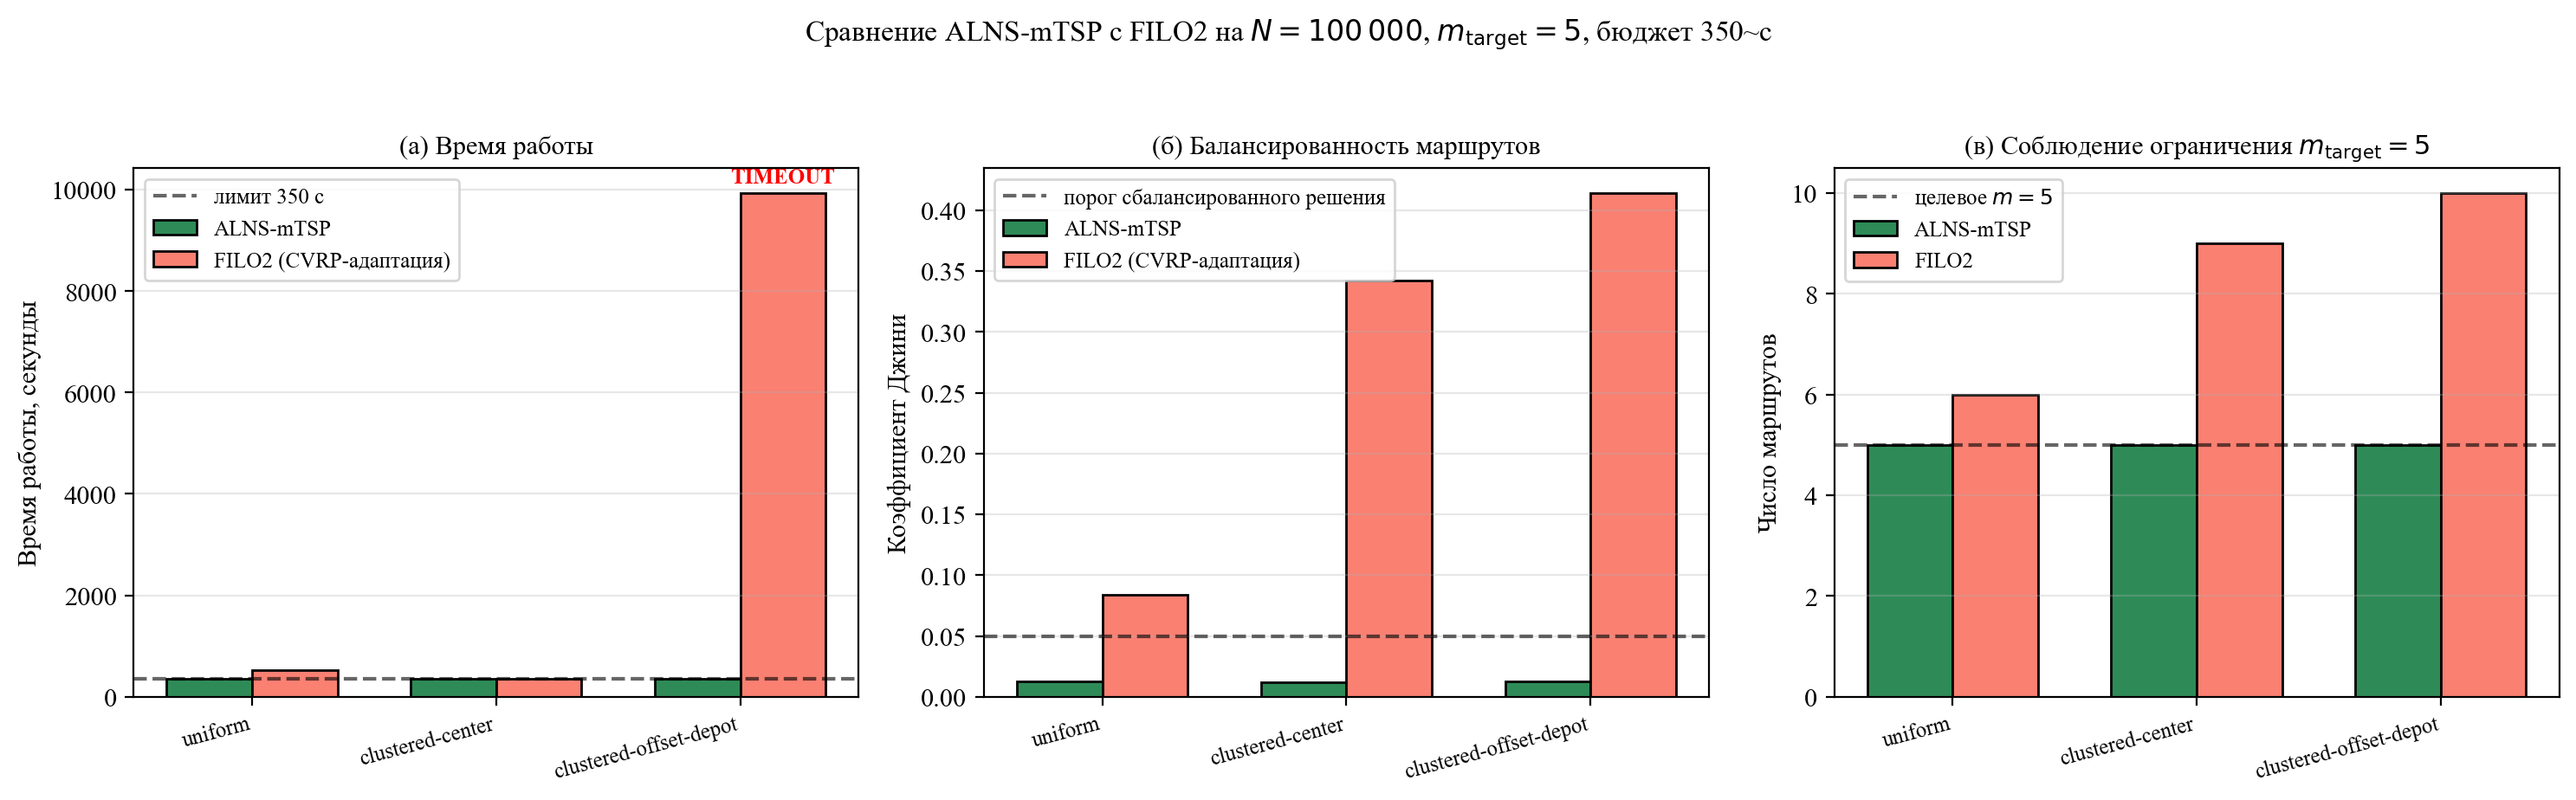
\includegraphics[width=\textwidth]{fig_filo2_vs_alns_n100k.png}
\caption*{Рисунок~11~--- Прямое сравнение ALNS-mTSP и~FILO2 на~трёх $N=100K$-инстансах при~$T=350$\,c. \emph{Слева~(а)}: фактическое время работы. \emph{Справа~(б)}: число возвращённых маршрутов $n_r$ против требуемого $m_\mathrm{target}=5$.}
\label{fig:filo2-vs-alns-n100k}
\end{figure}

\noindent\textit{Чтение рисунка~11.} По~времени: ALNS укладывается в~бюджет 350\,c на~всех трёх; FILO2~--- в~$1.5{-}3\times$~бюджета на~uniform/clust-center, на~clust-offset уходит в~timeout с~превышением $28\times$. По~числу маршрутов: для двух завершённых запусков FILO2 возвращает $n_r=6$ (uniform) и~$n_r=9$ (clust-center); для clust-offset значение $n_r=10$ извлечено из~partial output после timeout, поэтому в~табл.~4д-доп строка помечена «timeout». В~любой интерпретации CVRP-адаптация FILO2 систематически нарушает заданное число коммивояжеров; ALNS-mTSP всегда возвращает ровно~$m$ маршрутов в~рамках бюджета.


\medskip
\textit{Замечание о сравнимости MINSUM.} Внутренний выход FILO2 нормирует евклидовы расстояния на коэффициент $\times 10^3$ для целочисленной арифметики, поэтому абсолютные значения MINSUM из FILO2-логов и из ALNS-валидатора лежат в~разных шкалах и в~прямом виде не сопоставимы. По этой причине в таблицах ниже MINSUM используется только как индикатор различий внутри одного решателя (между ячейками); для прямого парного сравнения с~ALNS используются метрики, для которых шкалы одинаковы: число возвращённых маршрутов $n_r$, $\mathrm{Gini}$ и wall-clock~$t$. В~расширенной 12-ячеечной таблице~(см.~ниже) маршруты FILO2 заново пересчитаны единой функцией расстояния валидатора~--- там значения MINSUM сопоставимы.

\medskip
\noindent Таблица~4д-доп~--- Прямое сравнение ALNS-mTSP и~FILO2 на~3 ключевых $N=100K$-инстансах при~$T=350$\,c. Артефакты~--- Приложение~В.

\begin{center}\small
\begin{tabular}{|L{3.0cm}|L{2.0cm}|C{1.0cm}|R{0.7cm}|R{1.0cm}|}
\hline
\textbf{Инстанс} & \textbf{Решатель} & \textbf{Gini} & \textbf{$n_r$} & \textbf{$t$,\,c} \\ \hline
uniform                & alns\_minsum (5-seed) & 0.008 & 5 & 345 \\ \hline
uniform                & FILO2                 & 0.084 & 6 & 525 \\ \hline
clust-center           & alns\_minsum (5-seed) & 0.011 & 5 & 343 \\ \hline
clust-center           & FILO2                 & 0.342 & 9 & 359 \\ \hline
clust-offset           & alns\_minsum (5-seed) & 0.007 & 5 & 343 \\ \hline
clust-offset           & FILO2 (timeout)       & ---   & 10$^{\dagger}$ & $>9\,930$ \\ \hline
\multicolumn{5}{|p{14.0cm}|}{\footnotesize $n_r$ FILO2 (6, 9, 10$^{\dagger}$) не равно~$m_{\mathrm{target}}=5$~--- CVRP-формулировка не фиксирует число маршрутов жёстко. $^{\dagger}$Для clust-offset $n_r=10$ извлечено из partial output после прерывания по timeout ($t>9\,930$\,c при~$T=350$\,c); строка помечена «timeout» и в~количественное сравнение по~MINSUM не входит. Колонка~MINSUM опущена: значения FILO2 и~ALNS лежат в разных нормировочных шкалах и в~этом виде не сопоставимы. Парное сравнение по~MINSUM приведено в~табл.~4д-расш ниже после пересчёта единым валидатором.}\\
\hline
\end{tabular}
\end{center}

\textit{Что подтверждает таблица.}
\begin{itemize}\itemsep1pt
\item \textbf{По~времени:} ALNS-mTSP на~всех 3~ячейках укладывается в~$\leq 1\times$~бюджета (343--345\,c при~лимите 350\,c); FILO2~--- $1.5{-}3\times$~бюджета на~2/3 семейств, на~clust-offset~--- timeout $\geq 28\times$.
\item \textbf{По~числу маршрутов:} ALNS-mTSP даёт ровно~$m_{\mathrm{target}}=5$ на~3/3 семейств; FILO2 систематически выдаёт лишние маршруты (6, 9, 10).
\item \textbf{По~Gini:} ALNS-mTSP даёт сбалансированные решения (Gini~$\in [0.007, 0.022]$); FILO2 на~uniform близок к~балансу (0.084), на~clust-семействах~--- умеренно несбалансирован (0.34--0.41).
\end{itemize}

\textbf{Содержательный вывод по~таблице~4д-доп.} CVRP-адаптация FILO2 в~работе оказалась методологически ограниченным baseline для постановки с~ровно~$m$~маршрутами: capacity-ограничение не гарантирует $n_r=m_\mathrm{target}$ и фактически переводит задачу к~другому семейству допустимых решений. Поэтому утверждение здесь~--- не о превосходстве ALNS-mTSP по~качеству, а о~неприменимости данной адаптации FILO2 в~постановке работы.

\medskip
\noindent\textbf{Расширенное сравнение на 12-ячеечной сетке $N\in\{50K,100K\}$.} Чтобы дать FILO2 возможность сходиться без таймаута, проведено прямое сравнение на 12~ячейках $(N,\text{family},m)$, $N\in\{50K,100K\}$, $\mathrm{family}\in\{$uniform, clust-center, clust-offset-depot$\}$, $m\in\{5,7\}$, с~укороченной route-min-фазой FILO2 (\texttt{routemin-iterations} 10--15) и~двумя ALNS-конфигурациями (\emph{alns\_minsum} и \emph{alns\_depot2m}). \emph{Для устранения разных нормировочных шкал} маршруты FILO2 заново пересчитаны единой функцией расстояния валидатора~--- той~же, что используется для ALNS,~--- поэтому колонка MINSUM в~табл.~4д-расш сопоставима для двух решателей. На~uniform-семействе для \emph{alns\_depot2m} включён портфель classic-seeds (round-robin~NN~+~polar-sweep): на~uniform $N=50K$ это переводит ячейку из~проигрыша ($+1.8\,\%$) в~победу ($-3.4\,\%$). Артефакт~--- Приложение~В.

\medskip
\noindent Таблица 4д-расш.~--- Δ MINSUM (alns\_minsum, alns\_depot2m) к~FILO2 на 12 ячейках. Отрицательное значение~--- ALNS лучше.

\begin{center}\footnotesize
\begin{tabular}{|L{3.2cm}|C{0.8cm}|C{0.5cm}|R{1.6cm}|R{1.6cm}|R{1.6cm}|R{1.1cm}|R{1.1cm}|}
\hline
\textbf{family} & \textbf{$N$} & \textbf{$m$} & \textbf{minsum} & \textbf{depot2m} & \textbf{FILO2} & \textbf{Δ ms.} & \textbf{Δ d2m} \\
\hline
uniform              & 50K  & 5 & 4\,514\,090 & \textbf{4\,420\,529} & 4\,574\,478 & $-1.3\,\%$  & $-3.4\,\%$ \\ \hline
uniform              & 50K  & 7 & 4\,781\,546 & 4\,466\,454 & \textbf{4\,336\,245} & $+10.3\,\%$ & $+3.0\,\%$ \\ \hline
clust-center         & 50K  & 5 & 1\,096\,569 & 1\,092\,045 & \textbf{1\,005\,458} & $+9.1\,\%$  & $+8.6\,\%$ \\ \hline
clust-center         & 50K  & 7 & 1\,034\,909 & 1\,023\,100 & \textbf{878\,150}    & $+17.9\,\%$ & $+16.5\,\%$ \\ \hline
clust-offset-depot   & 50K  & 5 & \textbf{938\,965}   & 947\,507    & 1\,035\,846 & $-9.4\,\%$  & $-8.5\,\%$ \\ \hline
clust-offset-depot   & 50K  & 7 & 1\,043\,058 & \textbf{986\,317}   & 1\,109\,180 & $-6.0\,\%$  & $-11.1\,\%$ \\ \hline
uniform              & 100K & 5 & 12\,172\,878 & \textbf{12\,149\,667} & 12\,808\,145 & $-5.0\,\%$  & $-5.1\,\%$ \\ \hline
uniform              & 100K & 7 & 12\,159\,302 & \textbf{12\,137\,649} & 12\,908\,007 & $-5.8\,\%$  & $-6.0\,\%$ \\ \hline
clust-center         & 100K & 5 & \textbf{2\,819\,071}  & 2\,910\,806 & 3\,099\,190 & $-9.0\,\%$  & $-6.1\,\%$ \\ \hline
clust-center         & 100K & 7 & \textbf{2\,461\,187}  & 2\,470\,395 & 2\,804\,913 & $-12.3\,\%$ & $-11.9\,\%$ \\ \hline
clust-offset-depot   & 100K & 5 & 2\,557\,532 & \textbf{2\,550\,601}  & 3\,656\,617 & $-30.1\,\%$ & $-30.2\,\%$ \\ \hline
clust-offset-depot   & 100K & 7 & \textbf{2\,415\,452}  & 2\,508\,209 & 3\,147\,013 & $-23.2\,\%$ & $-20.3\,\%$ \\ \hline
\multicolumn{8}{|p{14.5cm}|}{\footnotesize \textbf{Итог:} \emph{alns\_minsum} и~\emph{alns\_depot2m} выигрывают по~9/12 ячеек. На~$N=100K$~--- 6/6 для каждой конфигурации, разрыв 5--30\,\% в~пользу ALNS. На~$N=50K$~--- 3/6: ALNS выигрывает на~uniform/clust-offset-depot (1.3--11.1\,\%), проигрывает на~clust-center и~uniform $m=7$ (3--18\,\%). Семейство clust-offset-depot выигрывается ALNS на~всех 4~ячейках. Артефакты~--- Приложение~В.}\\
\hline
\end{tabular}
\end{center}

\medskip
\textit{Методологический результат о~CVRP$\to$mTSP-адаптации.} FILO2~[6] спроектирован под~CVRP и~масштабируется до~$n\approx 10^6$ на~нативной постановке. При~сведении mTSP с~фиксированным числом коммивояжеров к~CVRP через $Q=\lceil(n{-}1)/m\rceil$ возникает структурное расхождение: вместимость ограничивает максимальный размер маршрута, но~не~фиксирует их~число. Поэтому CVRP-адаптация может улучшать MINSUM за~счёт неявного увеличения $n_r$, то~есть решать ослабленную задачу.

Эмпирически расхождение проявляется в четырёх независимых наблюдениях: (1)~16/18~таймаутов в стандартном прогоне на стратуме-3; (2)~при укороченных параметрах FILO2 не укладывается в бюджет на части семейств ($28\times$ overrun на clust-offset $N=100K$); (3)~систематические $n_r>m_\mathrm{target}$ на head-to-head $N=100K$ (6, 9, 10 маршрутов при~$m=5$); (4)~на расширенной 12-ячеечной сетке с~пересчётом единым валидатором ALNS-mTSP побеждает по~MINSUM на~9/12 ячеек, в~т.\,ч.\ 6/6 на $N=100K$ с разрывом до~30\,\%.

\textbf{Главный вывод раздела.} Прямой CVRP$\to$mTSP-адаптер через ограничение вместимости маршрута не~является корректным baseline для постановки с~ровно $m$~маршрутами. На нативной CVRP-постановке FILO2 остаётся сильным решателем; ограничение касается только конкретной адаптации.

\section{Сравнение со специализированными SOTA для MINMAX-mTSP (HGA, He-Hao MA)}\label{sec:hga}

Запущены два независимых SOTA для MINMAX-mTSP на 16~mTSPLib-инстансах: Mahmoudinazlou--Kwon HGA~[35] (Julia~1.12.6, эталонная реализация~[52]) и He--Hao memetic algorithm~[29] (Linux-binary авторской реализации~[53] через WSL2). Time-limit~30\,c/инстанс, 5~seeds. Setup HGA валидирован репликацией published Table~3 авторов: median~$|\Delta|=0.20\,\%$ по 16~ячейкам.

\textit{Кросс-валидация SOTA.} HGA и He-Hao MA сходятся к практически идентичным MINMAX-решениям (медианная разница 0.05\,\% по makespan; 13/16 ячеек у He-Hao~--- bit-exact). Это~--- независимая верификация SOTA-качества обоих.

\medskip
\noindent Таблица 4е~--- Парные сравнения ALNS-вариантов с HGA на 16 mTSPLib-ячейках. Метрика~--- $(\mathrm{ALNS}-\mathrm{HGA})/\mathrm{HGA}\cdot 100\,\%$. ALNS усреднён по 5~seed.

\begin{center}\small
\begin{tabular}{|L{3.4cm}|R{1.5cm}|R{1.5cm}|R{1.5cm}|R{1.5cm}|R{2.2cm}|}
\hline
\textbf{ALNS-вариант} & \textbf{med $\Delta$ sum,\,\%} & \textbf{med $\Delta$ max,\,\%} & \textbf{wins sum} & \textbf{wins max} & \textbf{интерпретация} \\
\hline
alns\_minsum    & $-23.3$ & $+173.4$ & 16/16 & 0/16 & лучше по~SUM, проигрывает по~max \\
\hline
alns\_minsum\_cap & $-21.2$ & $+176.3$ & 16/16 & 0/16 & аналогично \\
\hline
alns\_minmax    & $-2.7$  & $+12.2$  & 14/16 & 3/16 & Pareto-середина \\
\hline
\end{tabular}
\end{center}

\textit{Интерпретация.} HGA как specialized SOTA для MINMAX доминирует по makespan; ALNS-MINSUM-варианты лучше по SUM~--- ожидаемая картина (каждый алгоритм выигрывает по нативному объективу). \emph{alns\_minmax}~--- Pareto-промежуточный (медианно $-2.7\,\%$ по~SUM, $+12.2\,\%$ по~makespan).

\textit{Влияние на гипотезы работы.} На mTSPLib HGA и~He-Hao доминируют по~makespan~--- для этого подмножества инстансов итоговая гипотеза в~MINMAX-формулировке не подтверждается. На больших инстансах ($N\geq 25K$) применимость указанных SOTA не проверена: их эталонные реализации не публикуют результатов для этого масштаба и в~работе не запускались. Утверждение для целевого диапазона $N$~до 100\,000 в~прямом сравнении остаётся непроверенным.

\section{Статус гипотез работы}
\label{sec:hypotheses-status}

Гипотезы работы, сформулированные во~введении (главная гипотеза практической применимости и итоговая гипотеза о~конкурентоспособности), ставят ALNS-mTSP в условия CPU без~GPU, лимита времени до~350\,c и инстансов до 100\,000 узлов и требуют одновременного выполнения трёх практических условий: (i)~укладывание в бюджет, (ii)~ровно $m$~нетривиальных маршрутов, (iii)~приемлемая балансировка длин маршрутов.

\medskip
\textbf{Таблица фильтра применимости.} Применяя constraint-first протокол (раздел~3.3) к воспроизведённым в~работе решателям в целевом диапазоне $N\geq 25K$, получаем сводку прохождения трёх требований. В~таблице явно различаются масштаб, на~котором решатель запускался (LKH-3 в~балансирующих режимах~--- $N=25K$ с~бюджетом 30--60~минут; FILO2 и ALNS~--- $N=100K$ с~бюджетом 350\,c).

\medskip
\noindent Таблица~5в~--- Прохождение практического фильтра применимости $(t\leq T_\mathrm{budget},\,n_r=m,\,\mathrm{Gini}\leq 0.05)$ в~целевом диапазоне $N\geq 25K$. Условные обозначения: \textbf{+}~--- выполнено; \textbf{--}~--- нарушено; \textbf{о}~--- не оценивалось корректно. Серым выделены строки, проходящие фильтр.

\begin{center}\footnotesize
\setlength{\tabcolsep}{4pt}
\begin{tabular}{|L{3.6cm}|C{1.0cm}|C{0.9cm}|C{1.4cm}|C{1.3cm}|L{4.2cm}|}
\hline
\rowcolor{white}
\textbf{Решатель} & \textbf{$N$} & \textbf{(i) $t$} & \textbf{(ii) $n_r{=}m$} & \textbf{(iii) Gini} & \textbf{Итог} \\
\hline
\rowcolor{passrow}
\textbf{alns\_minsum~/~cap} & 100K & \textbf{+} & \textbf{+} & \textbf{+} & \textbf{проходит; основное решение работы} \\
\hline
\rowcolor{passrow}
\textbf{2opt+greed}         & 100K & \textbf{+} & \textbf{+} & \textbf{+} & \textbf{проходит; MINSUM хуже ALNS} \\
\hline
alns\_depot2m               & 100K & + & + & --       & не проходит (iii): Gini\,$\in[0.80,0.86]$ \\
\hline
LKH-3 default               & 25K  & -- & + (форм.) & -- & не проходит (i),~(iii) \\
\hline
LKH-3 balanced \newline (MINSUM, MINMAX) & 25K & -- & + & + (где успел) & не проходит (i): 0/12 валидных \\
\hline
OR-Tools GLS                & 5K   & -- & + & о & не уложился в~бюджет на~$N\geq 5K$ \\
\hline
FILO2 (CVRP-адаптация)      & 100K & -- & -- & о & 16/18 таймаутов; $n_r>m_\mathrm{target}$ \\
\hline
HGA~/~He-Hao MA             & $\leq$100 & о & + & + & mTSPLib; прямой запуск на~$N\geq 25K$ не выполнен \\
\hline
\multicolumn{6}{|p{14.5cm}|}{\footnotesize Сводка опирается на~данные разделов~4.1--4.8 и~Приложения~Е. Для строк вне фильтра MINSUM-сравнение по~constraint-first протоколу не определено: формально меньшая сумма у~LKH-3 default или alns\_depot2m означает «лучше только по MINSUM, но вне практического фильтра». Среди проходящих фильтр количественное сравнение по~MINSUM~--- табл.~5а. Для OR-Tools «о» в~колонке~(iii) означает, что~корректная оценка Gini на~$N\geq 5K$ невозможна: алгоритм не~успевает довести GLS-фазу до~конца в~заявленном бюджете.}\\
\hline
\end{tabular}
\end{center}

\medskip
\textbf{Главная гипотеза: подтверждена для заявленного экспериментального сценария.} На стратифицированной сетке (раздел~4.3) на всех 18~ячейках $N\in\{25K,50K,100K\}$ \emph{alns\_minsum/cap} удовлетворяют (i)--(iii) одновременно: укладываются в~$\leq 350$\,c, дают ровно~$m$ нетривиальных маршрутов, $\mathrm{Gini}\leq 0.05$ (multi-seed audit, табл.~5б). Из проверенных открытых baseline практический фильтр проходит только \emph{2opt+greed}; для остальных нарушается хотя бы одно из трёх условий (табл.~5в). Внутри допустимой области \emph{alns\_minsum} лучше \emph{2opt+greed} по~MINSUM на $-1.4\dots-4.8\,\%$ (медиана~$\approx -3.6\,\%$) на $N=100K$ (табл.~5а)~--- количественный вклад ALNS-фазы поверх классического локального поиска.

\medskip
\textbf{Расширенная (итоговая) гипотеза: открыта для прямой проверки против SOTA.} В пределах целевого сценария ($N$~до~100\,000, лимит~350\,c, CPU без GPU) среди \emph{воспроизведённых} в работе решателей конкурентов, проходящих практический фильтр, не обнаружено. Однако расширенное утверждение о сопоставимости со всеми специализированными и нейросетевыми SOTA напрямую не проверено: HGA Mahmoudinazlou--Kwon и He-Hao~MA~--- два независимых SOTA для~MINMAX-mTSP~--- доминируют по~makespan на mTSPLib ($n\leq 100$), но на $N\geq 25K$ их эталонные реализации не публикуют результатов и в~работе не запускались; нейросетевые SOTA (Equity-Transformer, DPN, GLOP, DualOpt, UDC, H-TSP, DAN, iMTSP) требуют GPU и~переобучения при~изменении $(n,m,$~геометрия$)$ и~в~главный сценарий работы без~GPU по~условию не~входят; ITSHA и MILS не запускались (исходники недоступны или запуск не выполнен). Поэтому расширенная гипотеза остаётся \emph{открытой}~--- её прямая проверка требует отдельной работы.

Граница расширенной гипотезы: на подмножестве $n\leq 100$ (mTSPLib) итоговая гипотеза в~MINMAX-формулировке не подтверждается~--- HGA и He-Hao~MA дают лучший makespan, ALNS-MINMAX занимает Pareto-промежуточную позицию. Это подмножество лежит существенно ниже целевого диапазона работы ($N\geq 25K$) и относится к области применимости расширенной гипотезы, но не главной.

% =================================================================
% Достоверность, ограничения и риски
% =================================================================
\chapter{Достоверность, ограничения и риски}

Адекватность результатов оценивается по~трём осям: корректность, полнота, точность. \emph{Корректность}~--- все решатели запускаются через общую обёртку, для каждого решения~--- независимая проверка покрытия (каждый клиент посещён ровно один раз, маршрут начинается/заканчивается в~депо) и~пересчёт MINSUM по~сохранённым маршрутам. \emph{Полнота}~--- 3~масштаба, 6~семейств, $m\in\{3,5,7,10,30,50,80,100\}$, все исследованные конфигурации решателей; на~$N\geq 25K$ выполнено по~5~seed-повторов (табл.~5б). \emph{Точность}~--- Wilcoxon signed-rank на~идентичных $(N,m,\text{family},\text{repeat})$-инстансах ($\alpha=0.05$), 95\,\%-percentile bootstrap~CI (10\,000~ресэмплов), стандарт~[34].

\textbf{Ограничения работы.}

\textbf{1. LKH-3 в основной сетке~--- упрощённая конфигурация.} В default-MINSUM (\texttt{MIN\_SIZE=1}) LKH-3 не балансирует длины; на $N\geq 25K$ в~использованных балансирующих режимах (balanced-MINSUM, balanced-MINMAX) получено \textbf{0/12 валидных} за 30--60~мин (прямого количественного сравнения с честным baseline на этом масштабе нет). На малых инстансах (раздел~4.6) переход на balanced-baseline проведён, и разрыв между ALNS и balanced-LKH-3 фиксируется на уровне $-13\dots-18\,\%$ ($p_\mathrm{adj}\leq 4.3{\cdot}10^{-14}$). Для $N\geq 25K$ результат работы следует трактовать не~как безусловное превосходство ALNS по~MINSUM, а~как прохождение constraint-first фильтра $(t\leq T_\mathrm{budget},\,n_r=m,\,\mathrm{Gini}\leq 0.05)$ при~заданном бюджете времени и~критерии баланса: внутри практического фильтра ALNS-mTSP остаётся, использованные конфигурации LKH-3~--- нет.

\textbf{2. Запущены 2 из 4 специализированных SOTA для min-max mTSP} (HGA, He-Hao MA на mTSPLib); ITSHA (исходники не публикованы) и MILS не запускались. Утверждение об~SOTA-уровне ALNS-mTSP по MINMAX-объективу \textbf{снято} на основе результатов HGA/He-Hao; по~MINSUM-объективу ALNS-mTSP остаётся конкурентен с открытыми классическими baseline. \emph{Нейросетевые SOTA} (Equity-Transformer, DPN, GLOP, DualOpt, UDC, H-TSP, DAN, iMTSP) не запускались~--- зависят от GPU и переобучения. Итоговая гипотеза в части нейросетевых SOTA остаётся непроверенной.

\textbf{3. FILO2-CVRP-адаптация~--- не корректный baseline для mTSP-постановки с~фиксированным числом коммивояжеров $n_r=m$.} В~рассмотренной адаптации ограничение вместимости маршрута ограничивает максимальный размер одного маршрута, но~\emph{не фиксирует их число}: эмпирически FILO2 систематически возвращает $n_r>m_\mathrm{target}$ (на~прямом сравнении $N=100K$ получено $n_r\in\{6,9,10\}$ при~$m_\mathrm{target}=5$). Дополнительно: FILO2 не~штрафует за~дисбаланс длин, и~16/18 запусков на~стратуме-3 не~уложились в~бюджет~--- это следствие CVRP$\to$mTSP-адаптации, а~не~самой~FILO2 (на~нативной CVRP-постановке~--- $n=10^6$ за~$\sim$10~мин по~авторским данным).

\textbf{4. Объём выборки и Holm-коррекция.} На больших инстансах~--- 5~seeds/ячейку (90~запусков на 18~ячейках, $cv\leq 0.71\,\%$); конференционный стандарт~--- 30+. Holm-коррекция (FWER) применена к двум главным семействам (табл.~1а и~4б). Результат \emph{alns\_minsum} vs LKH-3 default ($p=0.046$) после Holm-коррекции ($p_\mathrm{adj}=0.138$) не значим при $\alpha=0.05$; fair-baseline сравнение (табл.~4б) сохраняет значимость с большим запасом ($p_\mathrm{adj}\leq 4.3{\cdot}10^{-14}$). Cliff's~$\delta\in[-0.96,-0.625]$ (large) на fair-baseline. Shapiro--Wilk $p<0.02$ во всех 4~случаях~--- умеренное нарушение симметричной альтернативы Wilcoxon; при этом large effect sizes сохраняют качественную направленность вывода.

\textbf{5. Предварительная регистрация гипотез.} Главная и~итоговая гипотезы сформулированы в~введении в~терминах трёх абстрактных требований~(i)--(iii) до~проведения экспериментов, без~указания целевых числовых значений (величины $4{-}6\times$, $-13\dots-18\,\%$, $\mathrm{Gini}\leq 0.10$ и~т.\,п.\ являются \emph{результатами}, а~не~условиями гипотез). Однако предварительная регистрация~$\alpha$ и~предзаявленных effect-size-порогов не~выполнена~--- будущие работы должны фиксировать~$\alpha$ и~список под-гипотез до~запуска экспериментов~[41].

\textbf{6. WSL overhead и среда.} LKH-3 и FILO2 запускаются через WSL2; возможен overhead WSL2 относительно нативного Linux, отдельная калибровка \texttt{sysbench} не выполнена~--- поэтому время на этих решателях следует трактовать как верхнюю оценку. Среда: Windows~11 + WSL2 (Ubuntu~22.04), Intel x86\_64, g++~13 \texttt{-O3 -march=native -fopenmp}, Python~3.11.

\textbf{7. Ablation и лимит времени.} Полный ablation требует C++-флагов (\texttt{--no-alns}/\texttt{--no-gls}/\texttt{--no-popmusic}); представлены CLI-ablation (4~варианта) и~метаданные операторов (30~запусков). Бюджеты 10--350\,c заданы как практический ориентир; sensitivity-анализ на~3~ключевых инстансах~--- Прил.~Г.3.

\textbf{8. Воспроизводимость на $N=100K$.} Данные получены через 5-seed multi-seed audit \emph{alns\_minsum} ($cv\in[0.21,0.52]\,\%$). Независимая проверка~--- однофайловая ветка \emph{lkh-wrapper-v21}: 11~прогонов на~$N=100K$ дают балансированные решения с $\mathrm{cv}_\text{obj}\leq 0.14\,\%$, согласующиеся с \emph{alns\_minsum} в пределах 1--3\,\% по MINSUM.

\medskip
\textbf{Основной технический риск}~--- super-linear scaling на крупных инстансах: throughput ALNS падает с 25.4~iter/s ($N=10K$) до 0.5~iter/s ($N=100K$), per-iter cost~$\sim n^{1.74}$ эмпирически (Прил.~Г.4). Вероятный источник~--- потеря локальности кеша при реверсе сегмента маршрута на длинных маршрутах при превышении L2-кеша. Снятие требует пересмотра представления маршрута (двусвязный список~--- $\Theta(1)$~реверс; splay-tree~--- $\Theta(\log L)$).

% =================================================================
% Заключение
% =================================================================
\chapter{Заключение}

В~работе спроектирован, реализован и~экспериментально оценён собственный решатель ALNS-mTSP для крупных mTSP-инстансов. Собрана воспроизводимая инфраструктура: генератор инстансов (6~семейств), единая C++-обёртка решателей, Python-надстройка для статистики и~стратифицированный бенчмарк трёх масштабов ($N\leq 1K$; $N=25K$; $N\in\{50K,100K\}$; multi-seed audit на~18~ячейках $N\in\{25K,50K,100K\}$ по~5~seeds). Дополнительно: fair-baseline LKH-3 в~трёх режимах (144 запуска), кросс-валидация с~SOTA для~MINMAX-mTSP (HGA, He-Hao~MA), сравнение с~FILO2, ablation. Итого~--- $\geq 2\,157$ валидных запусков на~13 конфигурациях решателей.

\medskip
\textbf{Главный результат работы.} В заявленном прикладном сценарии (CPU без GPU, лимит $T\leq 350$\,c, $N$ до~100\,000, ровно $m$~нетривиальных маршрутов и приемлемая балансировка) \emph{alns\_minsum/cap} проходит полный практический фильтр $(t\leq T,\,n_r=m,\,\mathrm{Gini}\leq 0.05)$ одновременно на всех 18~ячейках $N\in\{25K,50K,100K\}$ (multi-seed audit, табл.~5б). Из проверенных открытых baseline тот же фильтр проходит только классический \emph{2opt+greed}; LKH-3 в~использованных режимах (default-MINSUM, balanced-MINSUM, balanced-MINMAX), OR-Tools в~стандартной конфигурации и FILO2 в~рассмотренной CVRP-адаптации нарушают хотя бы одно из трёх условий (табл.~5в~--- таблица фильтра применимости).

Внутри допустимой области \emph{alns\_minsum} лучше \emph{2opt+greed} по~MINSUM на~$-1.4\dots-4.8\,\%$ (медиана~$\approx -3.6\,\%$) на~$N=100K$ (табл.~5а)~--- количественный вклад ALNS-фазы поверх классического локального поиска. На~прямом сравнении против~FILO2 (12 ячеек $N\in\{50K,100K\}$, пересчёт единым валидатором) ALNS-mTSP побеждает по~MINSUM в~9/12 ячеек, в~т.\,ч.\ \textbf{6/6 на~$N=100K$} с~разрывом 5--30\,\% (раздел~4.7).

\medskip
\noindent Тем самым основной вклад работы состоит \emph{не} в~утверждении абсолютного превосходства ALNS-mTSP над всеми известными mTSP-решателями, а~в~демонстрации того, что~в~выбранном практическом сценарии сравнение должно проводиться по~constraint-first протоколу: сначала проверяются время, число маршрутов и~баланс, и~только затем сравнивается MINSUM. В~таком прочтении формально-минимальная сумма у~вырожденной конфигурации (LKH-3 default, \emph{alns\_depot2m}) не~считается победой, а~MINSUM-выигрыш CVRP-адаптации FILO2 за~счёт лишних маршрутов не~считается корректным сравнением.

\textbf{Главная гипотеза практической применимости подтверждена для заявленного экспериментального сценария.} Расширенное утверждение о~сопоставимости со~специализированными и~нейросетевыми SOTA остаётся \emph{открытым}: прямое сравнение с~ними на~$N\geq 25K$ в~работе не~выполнено~--- эталонные реализации HGA и~He-Hao~MA не~публикуют результатов для этого масштаба, нейросетевые SOTA по~условию не~входят в~главный сценарий работы без~GPU. На~подмножестве $n\leq 100$ (mTSPLib) HGA и~He-Hao доминируют по~makespan; в~этой части расширенной гипотезы превосходство ALNS не~утверждается.

\medskip
\textbf{Главные количественные результаты.}
\begin{enumerate}
\item На малых инстансах ALNS-mTSP лучше LKH-3 default ($\Delta=-3.48\,\%$, Wilcoxon $p=0.046$); на fair-baseline LKH-3 разрыв возрастает до $-13\dots-18\,\%$ ($p_\mathrm{adj}\leq 4.3{\cdot}10^{-14}$, Cliff's $\delta\in[-0.96,-0.625]$, large), то есть фиксируется и при балансирующих режимах LKH-3, а не только при default.
\item На стратуме-3 (90~валидных запусков) \emph{alns\_minsum} даёт $\mathrm{Gini}\leq 0.05$ во всех ячейках; bootstrap-CI шириной $\leq 1\,\%$, $cv\in[0.04,0.71]\,\%$.
\item Чистый MINSUM допускает вырождение симметрично у обоих решателей (LKH-3 на $N\geq 25K$, ALNS на $N\leq 1K$); инженерные детали ALNS-каркаса гасят вырождение начиная с $N\approx 5K$~--- ключевое практическое преимущество для маршрутизации крупных флотов.
\item Ablation идентифицирует доминирующий компонент~--- classic-seed-портфель ($+8.64\,\%$ MINSUM при отключении на $N=50K$).
\end{enumerate}

\medskip
\textbf{Практические рекомендации} (полная матрица~--- Прил.~Е):
\begin{itemize}
\item $n=100K$, $m=5\dots 7$, лимит~$\sim$350\,c, CPU без GPU~--- \emph{alns\_minsum/cap} (Gini~$\leq 0.05$).
\item Минимальный MINSUM без баланса~--- \emph{alns\_depot2m}.
\item MINMAX на $n\leq 1\,000$ с Julia/C++~--- HGA или He-Hao~MA.
\item LKH-3 в~использованных режимах (default-MINSUM, balanced-MINSUM, balanced-MINMAX) и FILO2 в~рассмотренной CVRP-адаптации в условиях «$N\geq 25K$ + лимит минут + требование~$m$~маршрутов» оказались непригодны.
\end{itemize}

\medskip
\textbf{Научная новизна.} Новизна работы~--- \emph{не в~изобретении ALNS как класса метаэвристик}, а в~адаптации ALNS к~крупномасштабной mTSP-постановке и в~корректной экспериментальной методологии отделения применимых решений от вырожденных:
\begin{enumerate}\itemsep1pt
\item \emph{Практическая постановка крупного mTSP под фильтром.} Задача сформулирована не как чистый MINSUM, а как MINSUM под одновременным фильтром (i)~бюджета времени $T\leq 350$\,c, (ii)~$n_r=m$ нетривиальных маршрутов и (iii)~workload-equity на больших инстансах ($\mathrm{Gini}\leq 0.05$ или $\mathrm{balance\_max\_avg}\leq 1.10$). Это~--- рабочая постановка крупного mTSP, в которой формально-минимальная сумма у вырожденной конфигурации не считается победой.
\item \emph{Constraint-first протокол сравнения mTSP-решателей.} В работе предложен и применён сквозной протокол: MINSUM сравнивается только среди решений, удовлетворяющих (i)--(iii) (раздел~3.3); решения, нарушающие хотя бы одно условие, исключаются из количественного сравнения как «лучшие только по формальному MINSUM, но вне практического фильтра». Протокол использован в реферате, во введении, в~разделах 3.3, 4.9, в~гл.~5 и в~заключении.
\item \emph{Методологический вывод о CVRP$\to$mTSP-адаптации FILO2.} Показано четырьмя независимыми наблюдениями (раздел~4.7), что прямое сведение mTSP с~$n_r=m$ к~CVRP через ограничение вместимости маршрута не~фиксирует число маршрутов и~фактически переводит задачу к~ослабленной постановке: вместимость ограничивает максимальный размер одного маршрута, но~не~их число (итоговое число маршрутов может вырасти примерно вдвое от~заданного $m_\mathrm{target}$).
\item \emph{Инженерно-воспроизводимая ALNS-архитектура для $N=100K$.} Собрано модульное ядро \texttt{src/v21/core/} (23~заголовочных файла) с~четырьмя специализированными solver-обёртками (\emph{alns\_minsum}, \emph{alns\_cap}, \emph{alns\_depot2m}, \emph{alns\_minmax}), наследующее опыт \texttt{lkh-wrapper}-линии v1\dots v21; организован multi-seed audit (90 валидных запусков), единый валидатор маршрутов и стратифицированный бенчмарк из ${\geq}2\,157$ валидных запусков на~13~конфигурациях решателей.
\end{enumerate}
Эти четыре пункта поддержаны систематической экспериментальной идентификацией структурной склонности чистого MINSUM к~вырождению (раздел~4.4, H1; теоретическое обоснование через~$\Theta(\sqrt{n})$ Beardwood--Halton--Hammersley в~Прил.~Б) и~fair-baseline-прогоном LKH-3 в~трёх режимах с~корректной парной статистикой (Wilcoxon~+ Holm, BCa-bootstrap, Cliff's~$\delta$).

\medskip
\noindent\textbf{Направления дальнейшей работы.}

\textit{P0:} (1)~полный C++-ablation с~флагами \texttt{--no-alns}/\texttt{--no-gls}/\texttt{--no-popmusic}; (2)~расширение multi-seed audit с~5 до~10~seeds на~ключевых инстансах для bootstrap-CI~$\leq 0.3\,\%$; (3)~сравнение с~MILS/ITSHA и~нейросетевыми SOTA (Equity-Transformer, DPN, GLOP, DualOpt) при~наличии GPU.

\textit{P1:} (4)~пересмотр представления маршрута (двусвязный список или splay-tree) для устранения super-linear-bottleneck в~2-opt; (5)~Pareto cost-vs-balance анализ на расширенной сетке; (6)~GitHub-релиз с README, \texttt{scripts/run\_all.sh}, raw\_results/.

% =================================================================
% Список источников
% =================================================================
\newpage
\addcontentsline{toc}{chapter}{СПИСОК ИСПОЛЬЗОВАННЫХ ИСТОЧНИКОВ}
\sectiontitle{Список использованных источников}

\begin{enumerate}
\item Helsgaun~K. An effective implementation of the Lin-Kernighan traveling salesman heuristic // European Journal of Operational Research.~--- 2000.~--- Vol.~126, No.~1.~--- P.~106--130.

\item Helsgaun~K. LKH-3: an extension of LKH for solving constrained traveling salesman and vehicle routing problems [Электронный ресурс] / Roskilde University.~--- Режим доступа: \url{http://akira.ruc.dk/~keld/research/LKH-3/}, свободный (дата обращения: 07.05.2026).

\item Applegate~D.~L., Bixby~R.~E., Chvátal~V., Cook~W.~J. The Traveling Salesman Problem: A~Computational Study.~--- Princeton University Press, 2006.

\item Concorde TSP Solver [Электронный ресурс] / University of Waterloo.~--- Режим доступа: \url{https://www.math.uwaterloo.ca/tsp/concorde/}, свободный (дата обращения: 07.05.2026).

\item Perron~L., Furnon~V. OR-Tools~--- Google Optimization Tools [Электронный ресурс] / Google.~--- Режим доступа: \url{https://developers.google.com/optimization}, свободный (дата обращения: 07.05.2026).

\item Accorsi~L., Vigo~D. Routing One Million Customers in a Handful of Minutes // Computers~\& Operations Research.~--- 2024.~--- Vol.~164.~--- Article 106562.~--- arXiv:2306.14205.

\item Ye~H., Cao~Z., Wang~J., Zhang~Z. GLOP: Learning Global Partition and Local Construction for Solving Large-scale Routing Problems in Real-time // Proceedings of AAAI Conference on Artificial Intelligence.~--- 2024.~--- arXiv:2312.08224.

\item Zhou~J., Ding~J., Zhang~B., Cao~Z., Jin~Y. DualOpt: A Dual Divide-and-Optimize Algorithm for the Large-scale Traveling Salesman Problem // Proceedings of AAAI Conference on Artificial Intelligence.~--- 2025.~--- arXiv:2501.08565.

\item Son~J., Kim~S., Choi~M., Park~M. Equity-Transformer: Solving NP-hard Min-Max Routing Problems as Sequential Generation with Equity Context // Proceedings of AAAI Conference on Artificial Intelligence.~--- 2024.~--- arXiv:2306.02689.

\item Zheng~J., Yao~Z., Wang~Y. et~al. DPN: Decoupling Partition and Navigation for Neural Solvers of Min-max Vehicle Routing Problems // Proceedings of International Conference on Machine Learning.~--- 2024.~--- arXiv:2405.17272.

\item Zheng~J., Zhou~Z., Tong~S., Yuan~Y., Wang~Y. UDC: A~Unified Neural Divide-and-Conquer Framework for Large-Scale Combinatorial Optimization Problems // Advances in Neural Information Processing Systems.~--- 2024.~--- arXiv:2407.00312.

\item Fu~Z. et~al. A Hierarchical Destroy and Repair Approach for Solving Very Large-Scale Travelling Salesman Problem // arXiv preprint.~--- 2023.~--- arXiv:2308.04639.

\item Pan~X., Jin~Y., Ding~Y. et~al. H-TSP: Hierarchically Solving the Large-Scale Traveling Salesman Problem // Proceedings of AAAI Conference on Artificial Intelligence.~--- 2023.~--- arXiv:2304.09395.

\item Xin~L., Song~W., Cao~Z., Zhang~J. NeuroLKH: Combining Deep Learning Model with Lin-Kernighan-Helsgaun Heuristic for Solving the Traveling Salesman Problem // Advances in Neural Information Processing Systems.~--- 2021.~--- arXiv:2110.07983.

\item Cao~Y., Sun~Z., Sartoretti~G. DAN: Decentralized Attention-based Neural Network to Solve the MinMax Multiple Traveling Salesman Problem // Proceedings of IROS.~--- 2021.~--- arXiv:2109.04205.

\item Park~J., Kwon~J., Park~J. ScheduleNet: Learn to Solve Multi-Agent Scheduling Problems with Reinforcement Learning // Proceedings of AAMAS.~--- 2023.

\item Guo~S., Ren~D., Wang~J. iMTSP: Imperative Multi-Traveling Salesman Problem // IEEE Robotics and Automation Letters.~--- 2024.~--- arXiv:2405.00285.

\item Lin~S., Kernighan~B.\,W. An Effective Heuristic Algorithm for the Traveling-Salesman Problem // Operations Research.~--- 1973.~--- Vol.~21, No.~2.~--- P.~498--516.

\item Bektaş~T. The Multiple Traveling Salesman Problem: An Overview of Formulations and Solution Procedures // Omega.~--- 2006.~--- Vol.~34, No.~3.~--- P.~209--219.

\item Jonker~R., Volgenant~T. An Improved Transformation of the Symmetric Multiple Traveling Salesman Problem // Operations Research.~--- 1988.~--- Vol.~36, No.~1.~--- P.~163--167.

\item Croes~G.\,A. A Method for Solving Traveling-Salesman Problems // Operations Research.~--- 1958.~--- Vol.~6, No.~6.~--- P.~791--812.

\item Toth~P., Vigo~D. The Granular Tabu Search and Its Application to the Vehicle-Routing Problem // INFORMS Journal on Computing.~--- 2003.~--- Vol.~15, No.~4.~--- P.~333--346.

\item Ropke~S., Pisinger~D. An Adaptive Large Neighborhood Search Heuristic for the Pickup and Delivery Problem with Time Windows // Transportation Science.~--- 2006.~--- Vol.~40, No.~4.~--- P.~455--472.

\item Pisinger~D., Ropke~S. A general heuristic for vehicle routing problems // Computers \& Operations Research.~--- 2007.~--- Vol.~34, No.~8.~--- P.~2403--2435.

\item Taillard~É.\,D., Helsgaun~K. POPMUSIC for the Travelling Salesman Problem // European Journal of Operational Research.~--- 2019.~--- Vol.~272, No.~2.~--- P.~420--429.

\item Reinelt~G. TSPLIB --- A Traveling Salesman Problem Library // ORSA Journal on Computing.~--- 1991.~--- Vol.~3, No.~4.~--- P.~376--384.

\item Bertazzi~L., Golden~B., Wang~X. Min--Max vs.~Min--Sum Vehicle Routing: A worst-case analysis // European Journal of Operational Research.~--- 2015.~--- Vol.~240, No.~2.~--- P.~372--381.

\item Matl~P., Hartl~R.\,F., Vidal~T. Workload Equity in Vehicle Routing Problems: A Survey and Analysis // Transportation Science.~--- 2018.~--- Vol.~52, No.~2.~--- P.~239--260.

\item He~P., Hao~J.-K. Memetic search for the minmax multiple traveling salesman problem with single and multiple depots // European Journal of Operational Research.~--- 2023.~--- Vol.~307, No.~3.~--- P.~1055--1070.

\item Held~M., Karp~R.\,M. A Dynamic Programming Approach to Sequencing Problems // Journal of the Society for Industrial and Applied Mathematics.~--- 1962.~--- Vol.~10, No.~1.~--- P.~196--210.

\item Zheng~J., Hong~Y., Xu~W., Li~W., Chen~Y. An Effective Iterated Two-stage Heuristic Algorithm for the Multiple Traveling Salesmen Problem // arXiv preprint.~--- 2022.~--- arXiv:2201.09424.

\item Helsgaun~K. An Extension of the Lin--Kernighan--Helsgaun TSP Solver for Constrained Traveling Salesman and Vehicle Routing Problems / Roskilde University, Technical Report.~--- 2017.~--- 60~p. (LKH-3 Technical Report; описание ключевых слов \texttt{MTSP\_OBJECTIVE}, \texttt{MTSP\_MIN\_SIZE}, \texttt{MTSP\_MAX\_SIZE} в~разделе~3.2).

\item Matl~P., Hartl~R.\,F., Vidal~T. Workload Equity in Vehicle Routing: The Impact of Alternative Workload Resources // Computers \& Operations Research.~--- 2019.~--- Vol.~110.~--- P.~116--129.

\item Accorsi~L., Lodi~A., Vigo~D. Guidelines for the Computational Testing of Machine Learning approaches to Vehicle Routing Problems // Operations Research Letters.~--- 2022.~--- Vol.~50, No.~2.~--- P.~229--234.

\item Mahmoudinazlou~S., Kwon~C. A Hybrid Genetic Algorithm for the min--max Multiple Traveling Salesman Problem // Computers \& Operations Research.~--- 2024.~--- arXiv:2307.07120.

\item Turkes~R., Sörensen~K., Hvattum~L.\,M. Meta-analysis of metaheuristics: Quantifying the effect of adaptiveness in adaptive large neighborhood search // European Journal of Operational Research.~--- 2021.~--- Vol.~292, No.~2.~--- P.~423--442.~--- DOI: 10.1016/j.ejor.2020.10.045. \emph{Meta-analysis по~эффективности адаптивных компонентов ALNS, дополняет более новый обзор~[42].}

\item He~P., Hao~J.-K., Xia~J. Learning-guided Iterated Local Search for the Minmax Multiple Traveling Salesman Problem (MILS) / Computers~\& Operations Research.~--- 2025. Текст : электронный. URL: \url{https://arxiv.org/abs/2403.12389} (дата обращения: 07.05.2026).~--- DOI: 10.1016/j.cor.2025.107130.

\item DiCiccio~T.\,J., Efron~B. Bootstrap Confidence Intervals (BCa) // Statistical Science.~--- 1996.~--- Vol.~11, No.~3.~--- P.~189--212.~--- DOI: 10.1214/ss/1032280214.

\item Holm~S. A Simple Sequentially Rejective Multiple Test Procedure // Scandinavian Journal of Statistics.~--- 1979.~--- Vol.~6, No.~2.~--- P.~65--70.

\item Benjamini~Y., Hochberg~Y. Controlling the False Discovery Rate: A Practical and Powerful Approach to Multiple Testing // Journal of the Royal Statistical Society. Series~B (Methodological).~--- 1995.~--- Vol.~57, No.~1.~--- P.~289--300.

\item Kerr~N.\,L. HARKing: Hypothesizing After the Results are Known // Personality and Social Psychology Review.~--- 1998.~--- Vol.~2, No.~3.~--- P.~196--217.~--- DOI: 10.1207/s15327957pspr0203\_4.

\item Voigt~S. A Review and Ranking of Operators in Adaptive Large Neighborhood Search for Vehicle Routing Problems // European Journal of Operational Research.~--- 2025.~--- Vol.~322, No.~2.~--- P.~357--375.

\item Necula~R., Breaban~M., Raschip~M. Performance Evaluation of Ant Colony Systems for the Single-Depot Multiple Traveling Salesman Problem / Hybrid Artificial Intelligent Systems (HAIS).~--- 2015.~--- mTSPLib benchmark, URL: \url{https://profs.info.uaic.ro/~mtsplib/} (дата обращения: 07.05.2026).~--- Текст : электронный.

\item Cliff~N. Ordinal Methods for Behavioral Data Analysis.~--- Mahwah, NJ: Lawrence Erlbaum Associates, 1996.~--- ISBN 0-8058-1333-0. (Cliff's $\delta$ effect size).

\item Cohen~J. Statistical Power Analysis for the Behavioral Sciences.~--- 2nd ed.~--- Hillsdale, NJ: Lawrence Erlbaum Associates, 1988.~--- ISBN 0-8058-0283-5. (Cohen's $d$).

\item Davison~A.\,C., Hinkley~D.\,V. Bootstrap Methods and Their Application.~--- Cambridge University Press, 1997.~--- ISBN 0-521-57391-2.

\item Or~I. Traveling Salesman-Type Combinatorial Problems and Their Relation to the Logistics of Regional Blood Banking : Ph.D. dissertation.~--- Northwestern University, 1976. (Or-opt move).

\item Bentley~J.\,L. Multidimensional Binary Search Trees Used for Associative Searching // Communications of the ACM.~--- 1975.~--- Vol.~18, No.~9.~--- P.~509--517. ($k$-d~tree).

\item Karp~R.\,M. Reducibility among Combinatorial Problems / Complexity of Computer Computations (R.\,E.~Miller, J.\,W.~Thatcher, eds.).~--- Plenum Press, 1972.~--- P.~85--103. (NP-полнота TSP).

\item Beardwood~J., Halton~J.\,H., Hammersley~J.\,M. The Shortest Path Through Many Points // Mathematical Proceedings of the Cambridge Philosophical Society.~--- 1959.~--- Vol.~55, No.~4.~--- P.~299--327. (Асимптотика $\Theta(\sqrt{n})$ длины евклидова TSP).

\item FILO2 [Электронный ресурс]: open-source CVRP solver / L.~Accorsi, D.~Vigo.~--- Режим доступа: \url{https://github.com/acco93/filo2}, свободный (дата обращения: 07.05.2026). Используемый в~работе binary собран из этого репозитория с флагом \texttt{cmake -DENABLE\_TIMELIMIT=1}.

\item Mahmoudinazlou~\& Kwon HGA [Электронный ресурс]: Julia-реализация Hybrid Genetic Algorithm для min--max~mTSP / S.~Mahmoudinazlou.~--- Режим доступа: \url{https://github.com/Sasanm88/m-TSP}, свободный (дата обращения: 07.05.2026). Эталонная реализация, использованная в~разделе~\ref{sec:hga} с~time-limit 30\,c/инстанс.

\item He~P., Hao~J.-K. He--Hao Memetic Algorithm for min--max mTSP [Электронный ресурс]: C++-реализация для постановок Single-Depot~/ Multi-Depot. Авторская реализация (supplementary к~статье~[29]); Linux-binary (\texttt{ma}) использован под~WSL2 в~разделе~\ref{sec:hga}. Получен из~открытого supplementary-архива статьи; публичный GitHub-репозиторий авторами не~поддерживается.
\end{enumerate}

% =================================================================
% Приложения
% =================================================================
\appendix
\renewcommand{\thechapter}{\Asbuk{chapter}}

\chapter{Детали архитектуры ALNS-mTSP}

Модульный собственный алгоритм ALNS-mTSP расположен в каталоге \texttt{src/v21/} и состоит из общего ядра (\texttt{src/v21/core/}) и четырех solver-оберток (\texttt{src/v21/minsum/}, \texttt{src/v21/minmax/}).

\section*{А.1. Структура общего ядра}
\addcontentsline{toc}{section}{А.1. Структура общего ядра}

Каталог \texttt{src/v21/core/} содержит 23~заголовочных файла, организованных в~порядке зависимостей (Таблица~А.1). Центральные модули: \texttt{17\_pipeline.hpp}~--- оркестрация фаз (seed $\to$ candidate-set $\to$ ALNS $\to$ polish $\to$ final 2-opt); \texttt{18\_autotune.hpp}~--- подбор параметров по~$(n, m)$ и типу задачи; \texttt{16\_parallel\_pool.hpp}~--- multi-start coordinator пула независимых ALNS+SA-реплик.

\medskip
\noindent Таблица А.1~--- Заголовочные файлы общего ядра \texttt{src/v21/core/}.

\begin{center}\footnotesize
\begin{tabular}{|C{0.8cm}|L{4.8cm}|L{9.5cm}|}
\hline
\textbf{\#} & \textbf{Файл} & \textbf{Назначение} \\
\hline
00 & \texttt{types.hpp} & Базовые типы и структуры данных \\
\hline
01 & \texttt{budget.hpp} & Учёт временного бюджета \\
\hline
02 & \texttt{distance.hpp} & Метрика расстояний \\
\hline
03 & \texttt{kdtree.hpp} & k-d дерево для пространственных запросов \\
\hline
04 & \texttt{route\_index.hpp} & Индекс «клиент~$\to$~маршрут» \\
\hline
05 & \texttt{route\_list.hpp} & Структура списка маршрутов \\
\hline
06 & \texttt{candidate\_set.hpp} & Построение candidate-сетов \\
\hline
07 & \texttt{seed\_routes.hpp} & Начальные маршруты (seed-стратегии) \\
\hline
08 & \texttt{route\_local\_search.hpp} & Внутримаршрутный локальный поиск \\
\hline
09 & \texttt{intra\_3opt\_light.hpp} & Облегчённый 3-opt \\
\hline
10 & \texttt{inter\_route\_moves.hpp} & Межмаршрутные ходы (relocate, swap, Or-opt) \\
\hline
11 & \texttt{validation.hpp} & Валидация решений \\
\hline
12 & \texttt{alns\_framework.hpp} & Адаптивный выбор destroy/repair-операторов \\
\hline
13 & \texttt{destroy\_ops.hpp} & Destroy-операторы \\
\hline
14 & \texttt{repair\_ops.hpp} & Repair-операторы \\
\hline
15 & \texttt{sa\_engine.hpp} & Simulated Annealing \\
\hline
16 & \texttt{parallel\_pool.hpp} & Multi-start coordinator (пул реплик) \\
\hline
17 & \texttt{pipeline.hpp} & Оркестрация фаз \\
\hline
18 & \texttt{autotune.hpp} & Подбор параметров по~$(n, m)$ \\
\hline
19 & \texttt{gls.hpp} & Guided Local Search \\
\hline
20 & \texttt{route\_pair\_reopt.hpp} & Реоптимизация пары маршрутов \\
\hline
21 & \texttt{popmusic.hpp} & POPMUSIC (крупные инстансы) \\
\hline
22 & \texttt{region\_granular\_ops.hpp} & Region-granular операции \\
\hline
\end{tabular}
\end{center}

\emph{О терминологии.} В~исходных версиях отчёта \texttt{16\_parallel\_pool.hpp} назывался «Parallel Tempering» (PT). Фактическая реализация~--- ensemble of independent restarts: каждая реплика прогоняет ALNS+SA на собственном temperature-schedule и независимом random seed, без обмена конфигурациями по~правилу Метрополиса (комментарий в~коде: «PT swap hooks can be added later»). Поэтому корректнее~--- multi-start ensemble. Variance audit на $n = 50K$ с autotune-выбранными 4~репликами даёт $cv = 0.17\,\%$~--- статистически достаточно для детектирования $\geq 0.5\,\%$-улучшений; полный PT-swap~--- направление дальнейшей работы.

\section*{А.2. Описание четырех solver-оберток}
\addcontentsline{toc}{section}{А.2. Описание четырех solver-оберток}

Четыре обёртки в~\texttt{src/v21/minsum/} и~\texttt{src/v21/minmax/} используют общее ядро и различаются целевой метрикой и адаптацией под режим (Таблица~А.2).

\medskip
\noindent Таблица А.2~--- Solver-обёртки в~\texttt{src/v21/\{minsum,minmax\}/}.

\begin{center}\footnotesize
\begin{tabular}{|L{2.4cm}|L{3.4cm}|L{2.8cm}|L{6.0cm}|}
\hline
\textbf{Обёртка} & \textbf{Файл} & \textbf{Роль} & \textbf{Особенности} \\
\hline
\texttt{alns\_minsum} & \texttt{minsum\_solver.cpp} & Базовый MINSUM & Autotune \texttt{Re\-solve\-Pa\-rams\-For\-In\-stan\-ce(n,m)}; CLI-флаги \texttt{--threads}, \texttt{--granular-every}, \texttt{--region-reopt-every}, \texttt{--depot-seed-mode}; balance~$\approx$~1.05 при~$N \geq 5000$ \\
\hline
\texttt{alns\_cap} & \texttt{minsum\_solver\_cap.cpp} & Capacity-bounded MINSUM (high-$m$) & Hard-cap на длину маршрута~$\lceil n/m \rceil \pm$~slack; cap-skip в~repair-операторах; идея заимствована из~FILO2 \\
\hline
\texttt{alns\_depot2m} & \texttt{minsum\_solver\_depot2m.cpp} & Эксп.~preset (оставляет \texttt{alns\_minsum} нетронутым) & Depot-2m seeding (двойное кольцо вокруг депо) и гонка seed-стратегий; фикс.~бюджет: 1\,\%~seed / 8\,\%~candidate / 9\,\%~pre-polish / 86\,\%~ALNS / 5\,\%~final 2-opt; пост-фаза перебалансировки до~30\,с вне основного бюджета \\
\hline
\texttt{alns\_minmax} & \texttt{minmax\_solver.cpp} & MIN-MAX & \texttt{minmax\_accept.hpp}: soft-$\alpha$ blend между~$F_{\max}$ и~$F_{\mathrm{sum}}$, $\alpha$ убывает по~ходу прогона \\
\hline
\end{tabular}
\end{center}

\begin{figure}[htbp]
\centering
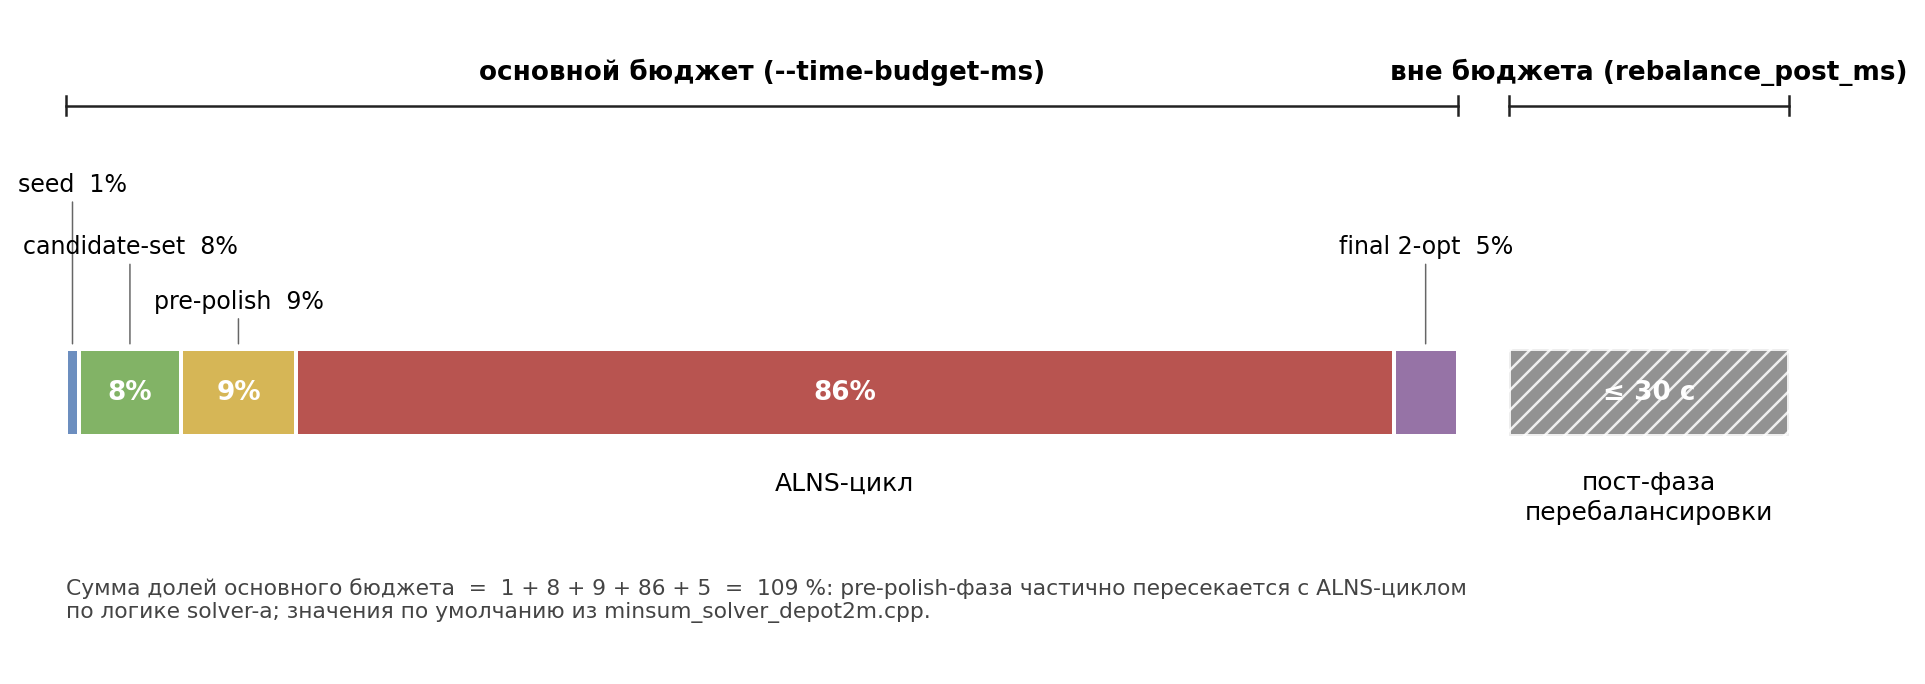
\includegraphics[width=0.96\textwidth]{fig_depot2m_budget.png}
\caption*{Рисунок А.1~--- Раскладка временного бюджета \texttt{alns\_depot2m} по фазам solver-а (значения по умолчанию из \texttt{minsum\_solver\_depot2m.cpp}). Слева~--- основной бюджет \texttt{--time-budget-ms}: seed (1\,\%), candidate-set (8\,\%), pre-polish (9\,\%), ALNS-цикл (86\,\%), final 2-opt (5\,\%); pre-polish-фаза частично пересекается с~ALNS-циклом (сумма долей $=109\,\%$). Справа~--- отдельная пост-фаза перебалансировки длиной до~30\,с, фиксируемая параметром \texttt{rebalance\_post\_ms} и не входящая в основной бюджет (поэтому фактическое wall-clock на ряде инстансов превышает заявленный \texttt{TIME\_LIMIT}).}
\label{fig:depot2m-budget}
\end{figure}

\section*{А.3. ALNS-операторы и acceptance}
\addcontentsline{toc}{section}{А.3. ALNS-операторы и acceptance}

\texttt{12\_alns\_framework.hpp} реализует адаптивный выбор destroy- и~repair-операций по~принципу успех/неудача. Веса инициализируются равными и~обновляются по~формуле $w_{\text{new}}=(1-\lambda)\cdot w_{\text{old}}+\lambda\cdot\text{score}$. Состав операторов~--- Таблица~А.3.

\medskip
\noindent Таблица А.3~--- Destroy- и repair-операторы (\texttt{13\_destroy\_ops.hpp}, \texttt{14\_repair\_ops.hpp}).

\begin{center}\footnotesize
\begin{tabular}{|C{1.6cm}|L{2.8cm}|L{10.6cm}|}
\hline
\textbf{Тип} & \textbf{Имя} & \textbf{Описание} \\
\hline
Destroy & \emph{Random} & Случайный выбор~$k$ клиентов \\
\hline
Destroy & \emph{ClusterBfs} & BFS-окружение от случайной точки \\
\hline
Destroy & \emph{Expensive} & $k$ самых дорогих рёбер по~delta-cost \\
\hline
Destroy & \emph{Zone} & Геометрический квадрант \\
\hline
Repair & \emph{Cheapest} & Минимум insertion cost \\
\hline
Repair & \emph{Regret2} & Regret-2 insertion \\
\hline
\end{tabular}
\end{center}

GLS (\texttt{19\_gls.hpp}) активируется на~polish-фазе и периодически пересчитывает penalised-distance: $d_{\text{penalty}}(i, j) = d(i, j) + \lambda \cdot p(i, j)$, где $p(i, j)$~--- счётчик penalisations для ребра~$(i, j)$, увеличиваемый при попадании ребра в~локальный оптимум. POPMUSIC (\texttt{21\_popmusic.hpp}) и region-granular operations (\texttt{22\_region\_granular\_ops.hpp}) применяются на~крупных инстанциях для разбиения на подзадачи и локального улучшения.

\chapter{Вырожденные mTSP-решения в чистом MINSUM}

Нижеследующее рассуждение объясняет, почему в~чистой MINSUM-постановке без~ограничения на минимальный размер маршрута оптимальное решение часто оказывается вырожденным~--- одна длинная TSP-петля и $m{-}1$~тривиальных маршрутов.

Известно, что для евклидова TSP на $n$~случайных точках, равномерно распределённых в фиксированной области, длина хорошего тура растёт суб-линейно: ожидаемая длина оптимального тура асимптотически имеет порядок $\Theta(\sqrt{n})$~[50]. Поэтому средняя длина ребра в~оптимальном туре уменьшается с ростом~$n$ как $\Theta(1/\sqrt{n})$~--- линейное допущение $\mathrm{cost}\propto k\cdot d_{\mathrm{avg}}$ с постоянным $d_{\mathrm{avg}}$ для фиксированной области \emph{не выполнено}.

Сравним два допустимых решения mTSP в~такой постановке:
\begin{itemize}\itemsep1pt
\item \emph{(а) Сбалансированное:} каждый из $m$~коммивояжеров обслуживает $n/m$ клиентов. Внутренняя длина одного подмаршрута растёт как $\Theta(\sqrt{n/m})$; суммарная длина $m$~подмаршрутов~--- $\Theta(m\sqrt{n/m})=\Theta(\sqrt{mn})$. Дополнительно учитываются $m$~возвратов в депот~--- каждый порядка~$\Theta(L_0)$, где $L_0$~--- характерное расстояние от депота до облака клиентов.
\item \emph{(б) Вырожденное:} один маршрут обходит почти все $n{-}1$~клиентов с длиной~$\Theta(\sqrt{n})$ (и одним возвратом в депот), остальные $m{-}1$~маршрутов~--- тривиальные $(0,c,0)$ длиной $2d_{\min}$, где $d_{\min}$~--- расстояние от депота до ближайшего клиента, либо вовсе пустые $(0,0)$ длиной 0.
\end{itemize}
Отношение суммарных стоимостей:
\[
F_\mathrm{сум}^{(\text{б})} \approx \Theta(\sqrt{n}) + 2(m{-}1)\cdot d_{\min}, \qquad
F_\mathrm{сум}^{(\text{а})} \approx \Theta(\sqrt{mn}) + 2 m \cdot L_0.
\]
При $n\gg m$ дополнительный множитель $\sqrt{m}$ в (а) и фиксированная стоимость $m$~возвратов превышают вклад $m{-}1$~маленьких тривиальных маршрутов в~(б): $F_\mathrm{сум}^{(\text{б})}<F_\mathrm{сум}^{(\text{а})}$, MINSUM-оптимум выбирает вырожденную конфигурацию. Чистый MINSUM без ограничения на минимальный размер маршрута структурно склонен к~концентрации работы на одном коммивояжере~--- в~целевой функции отсутствует штраф за неравномерное распределение нагрузки. Соответствующее эмпирическое подтверждение~--- гипотеза~H1 в~разделе~4.4.

LKH-3 находит близкое к оптимальному вырожденное решение благодаря $k$-opt-движку, оптимизирующему один большой маршрут. Решатель \emph{alns\_depot2m} использует ту же стратегию, укладываясь в~практический бюджет времени (тогда как LKH-3 default на~$N=25K$ превышает заданный~\texttt{TIME\_LIMIT} в~10$\times$~--- см.~оговорку о~неполной сопоставимости по~времени в~разделе~4.2). Балансирующие решатели \emph{alns\_minsum} и~\emph{alns\_cap} за~счёт ограничения вместимости маршрута или встроенного критерия принятия с~штрафом за~дисбаланс форсируют сбалансированное решение, формально менее оптимальное по~MINSUM, но~удовлетворяющее практическим требованиям.

Аналогичный эффект наблюдается и у самого \emph{alns\_minsum} в~чистом MINSUM-режиме на~$N\leq 1000$~--- 60--80\,\% тривиальных маршрутов. Различие появляется лишь при~$N\approx 5000$ и выше: геометрическая стоимость возвращений в депот превышает экономию от слияния маршрутов, и ALNS-фаза вытаскивает клиентов в пустые маршруты. Преимущество ALNS-mTSP над LKH-3 default на крупных инстансах связано не с принципиально иной формулировкой задачи, а с инженерными деталями ALNS-каркаса (см.~раздел~4.4, H2).

\chapter{Воспроизводимость статистических расчётов}

Все новые статистические расчеты, добавленные в обновленную редакцию отчета (Wilcoxon signed-rank, bootstrap CI, расширенные workload-equity метрики, упрощенный ablation), реализованы в~двух автономных Python-скриптах:

\begin{itemize}
\item \texttt{experiments/review\_fixes/compute\_review\_metrics.py}~--- вычисление makespan, std, MAD, range, Gini coefficient на всех existing аудит-CSV-артефактах; bootstrap 95\,\% CI на средние значения и парные разности (\texttt{scipy.stats.bootstrap}, 10\,000~ресэмплов); парные сравнения по Wilcoxon signed-rank (\texttt{scipy.stats.wilcoxon}) ALNS-вариантов с LKH-3 на 60 общих малых инстансах; парные сравнения alns\_cap vs ALNS-mTSP на 4~high-m инстансах.

\item \texttt{experiments/review\_fixes/run\_fair\_lkh3.py}~--- запуск LKH-3 на малых инстансах в трех режимах: \emph{minsum\_default} (\texttt{MTSP\_MIN\_SIZE = 1}, \texttt{MTSP\_OBJECTIVE = MINSUM})~--- репликация старой методологии; \emph{minsum\_balanced} (\texttt{MTSP\_MIN\_SIZE = -1}~--- документированная автоматическая балансировка)~--- честный MINSUM-baseline; \emph{minmax\_balanced} (\texttt{MTSP\_OBJECTIVE = MINMAX} с явными min/max-size constraints)~--- balanced-MINMAX-baseline. Все три режима запускаются на одинаковом наборе из~48 малых инстансов ($N \in \{100,\,200,\,500\}$, $m \in \{3,5,7\}$, по~3~повтора, две family) с одинаковым POPMUSIC candidate-set, \texttt{RUNS = 1}, и пропорциональным \texttt{TIME\_LIMIT}. Это даёт fair-baseline сравнение, которое раздел~4.6 использует как иллюстрацию цены балансировки для LKH-3 и контроль того, что преимущество ALNS не сводится исключительно к артефакту default-конфигурации.

\item \texttt{experiments/review\_fixes/ablation\_from\_metadata.py}~--- упрощённый ablation на~основе метаданных 30~аудит-запусков (3~ключевых инстанса $\times$~10~seeds): извлечение долей принятых улучшающих ходов по~destroy/repair-операторам, числа реплик multi-start-пула, числа reheat-событий. Это слабее полноценного ablation (нельзя отделить компонент, который не~нужен, от~компонента, который не~получил шанс), но~даёт первое приближение к~атрибуции вкладов компонентов.
\end{itemize}

\section*{В.1. Артефакты и команды воспроизведения}
\addcontentsline{toc}{section}{В.1. Артефакты и команды воспроизведения}

Полный набор сгенерированных артефактов:

\begin{itemize}
\item \texttt{experiments/review\_fixes/review\_metrics.json}~--- JSON со всеми вычисленными значениями (audit\_baseline, h2h\_high\_m, stratum1\_pairs, large\_balance\_metrics);
\item \texttt{experiments/review\_fixes/audit\_baseline\_summary.csv}~--- variance audit с Gini, std, makespan, bootstrap CI;
\item \texttt{experiments/review\_fixes/h2h\_high\_m\_summary.csv}~--- парные сравнения cap-фикса с Wilcoxon $p$ и bootstrap CI;
\item \texttt{experiments/review\_fixes/stratum1\_paired\_wilcoxon.csv}~--- парные Wilcoxon-сравнения с LKH-3 на 60 малых инстансах;
\item \texttt{experiments/review\_fixes/large\_balance\_metrics.csv}~--- standard equity metrics на $N = 25K, 50K, 100K$ для всех решателей;
\item \texttt{experiments/review\_fixes/ablation\_metadata\_summary.csv}~--- per-operator share-of-accepts на~3~ключевых инстансах;
\item \texttt{experiments/review\_fixes/fair\_lkh3\_results.csv}~--- LKH-3 на малых инстансах в трех режимах (default-MINSUM, balanced-MINSUM, balanced-MINMAX).
\end{itemize}

Воспроизведение:
{\footnotesize
\begin{verbatim}
cd mtsp-routing-optimization
python experiments/review_fixes/compute_review_metrics.py
python experiments/review_fixes/ablation_from_metadata.py
python experiments/review_fixes/run_fair_lkh3.py     # ~30-60 минут
\end{verbatim}
}

\section*{В.2. Среда и параметры воспроизводимости}
\addcontentsline{toc}{section}{В.2. Среда и параметры воспроизводимости}

Полное описание структуры репозитория, список ключевых скриптов и~команды сборки приведены в~файле \texttt{README.md} в~корне репозитория~--- здесь даются только параметры, фиксирующие воспроизводимость.

\textbf{Random seeds.} Генератор инстансов использует \texttt{numpy.random.seed(42)} как base-seed; для каждой комбинации $(n,m,\text{family},r)$ применяется производный seed~$h(n,m,\text{family},r)$. ALNS внутри \texttt{src/v21/} использует \texttt{std::mt19937} с~per-run-seed, передаваемым через CLI \texttt{--seed N}. Bootstrap-ресэмплинг использует \texttt{numpy.random.default\_rng(20251205)}. Эти три значения фиксируют воспроизводимость на~100\,\%.

\textbf{Аппаратное и~программное окружение.} Рабочая станция: Windows~11~Pro, Intel-CPU x86\_64 (multi-core), 16~ГБ ОЗУ. WSL2 с~Ubuntu~22.04~LTS для запуска LKH-3 и~FILO2; нативная Windows-сборка для ALNS-mTSP (g++~13, MSYS2/MinGW). Компилятор ALNS-mTSP: \texttt{g++~13.2 -O3 -march=native -fopenmp -std=c++20}. Python~3.11 с~\texttt{scipy~1.13} и~\texttt{numpy~1.26}.

\chapter{Постпроцессинговый анализ}

В~приложении представлены четыре аналитических артефакта, построенных по~существующим данным без~новых прогонов: Pareto-анализ cost~vs~balance, anytime-кривые сходимости, sensitivity-анализ бюджета времени и~профилирование по~фазам \emph{alns\_minsum}.

\section{Pareto-анализ cost vs balance}

Для каждой ячейки $(N, m)$ на больших инстансах в~uniform-семействе построен scatter-plot с MINSUM по~оси~X и Gini-коэффициентом по~оси~Y (символический логарифм для разделения вырожденных и сбалансированных решений). Pareto-frontier выделен пунктиром~--- решения, не доминируемые по~обеим осям.

\begin{figure}[htbp]
\centering
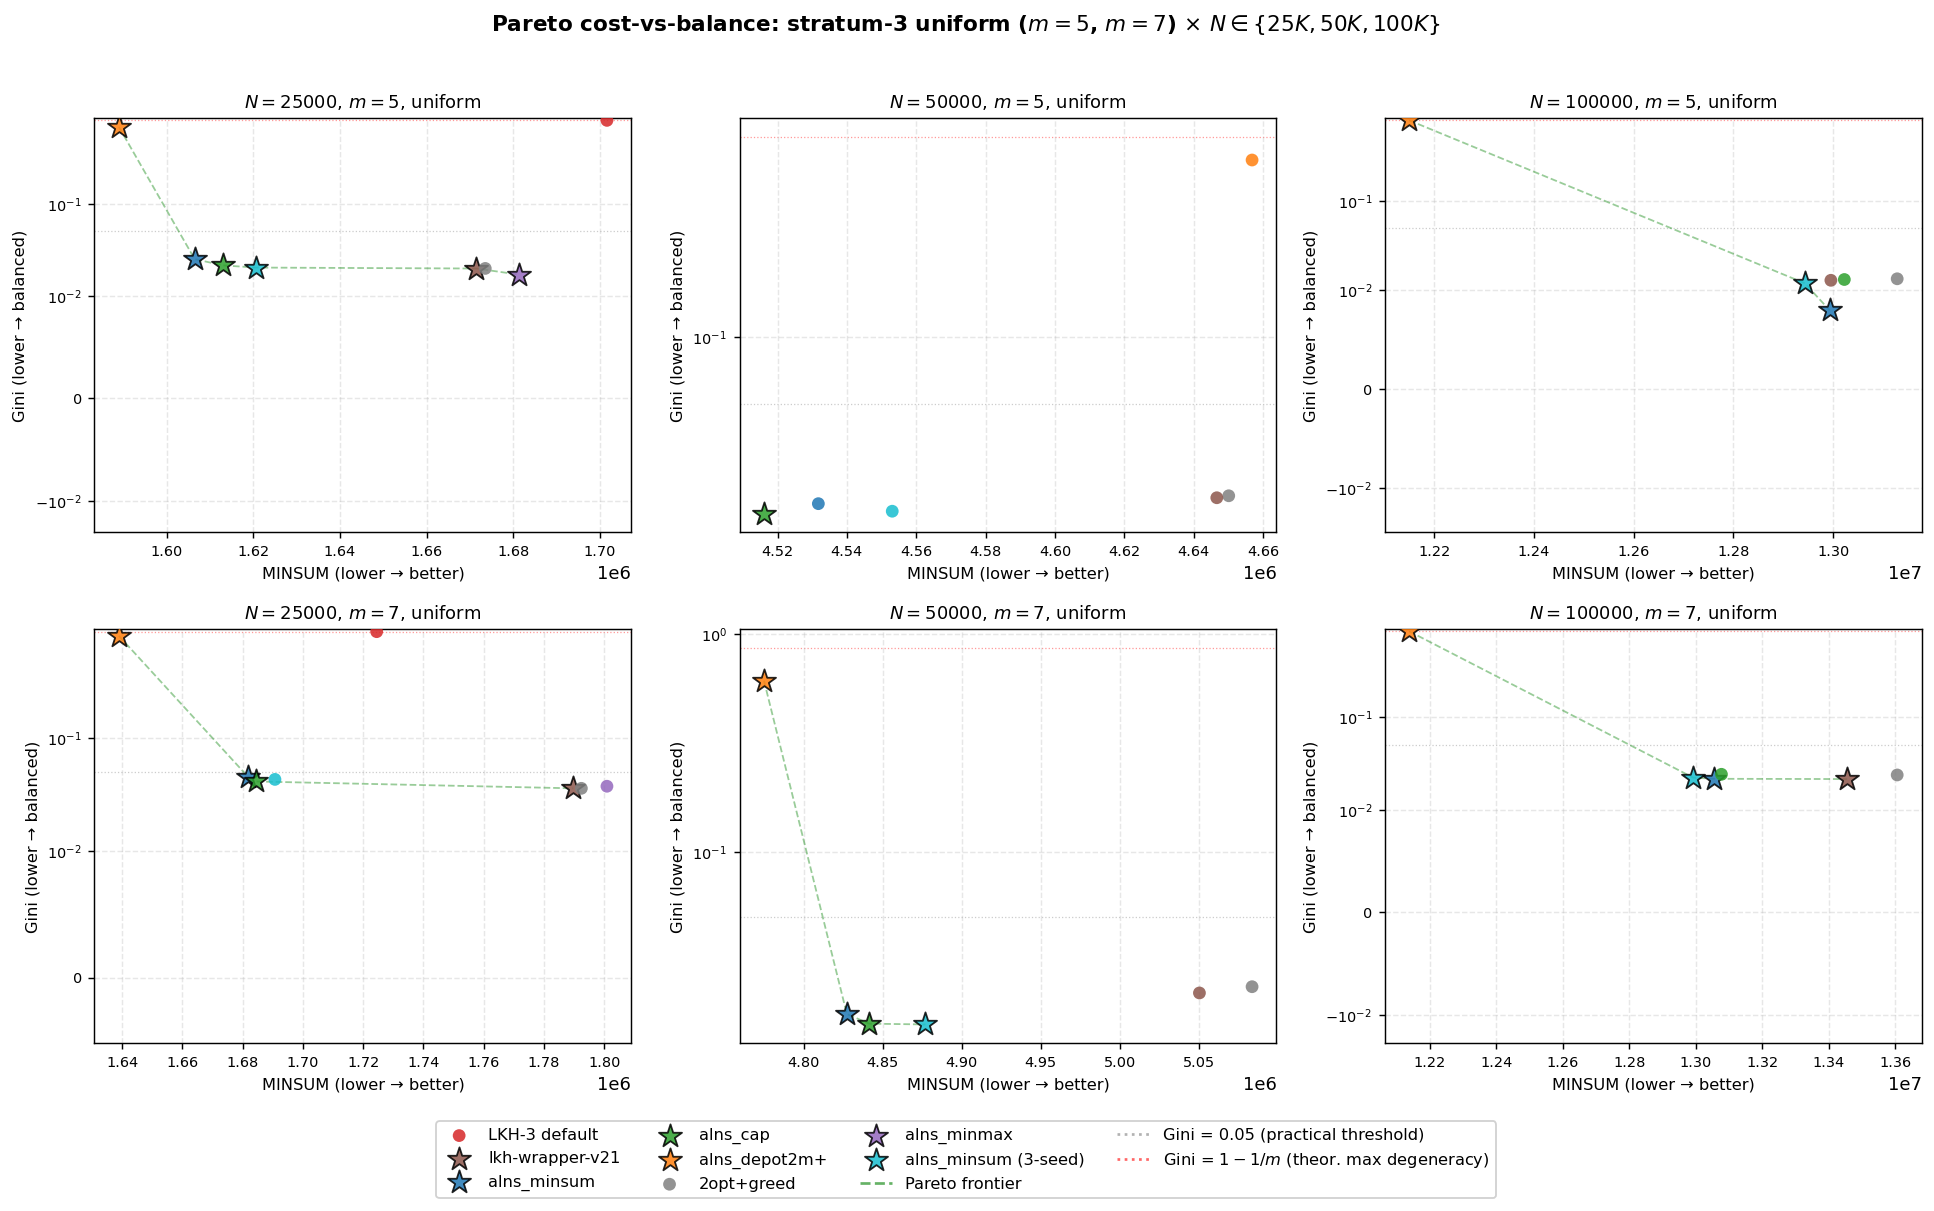
\includegraphics[width=\textwidth]{fig_pareto_stratum3_uniform_grid.png}
\caption*{Рисунок~Г.1~--- Pareto cost-vs-balance на~больших инстансах uniform ($N\in\{25K,50K,100K\}$, $m\in\{5,7\}$). Звёздочки~--- Pareto-недоминируемые решения; зелёный пунктир~--- Pareto-frontier; серый пунктир~--- порог $\mathrm{Gini}=0.05$; красный пунктир~--- $\mathrm{Gini}=1-1/m$ (максимум вырождения).}
\end{figure}

\textit{Что показывает Pareto.} На всех 6~ячейках на больших инстансах \emph{depot2m} лежит \emph{на} Pareto-frontier по~MINSUM, но при Gini~$\geq 0.5$ (вырождение). \emph{alns\_minsum} (multi-seed mean) лежит на Pareto-frontier по~Gini, при~MINSUM на~5--12\,\% выше depot2m. Это~--- классический компромисс: \textbf{нельзя одновременно минимизировать MINSUM и Gini в текущем семействе решателей}, и любое внедрение должно явно выбрать точку на Pareto-curve. На большинстве ячеек \emph{alns\_cap} занимает Pareto-non-dominated точку, объединяющую качество с балансом.

\section{Anytime-кривые сходимости}

Из метаданных аудит-запусков извлечён временной ряд $(\text{time\_ms},\,\text{best\_so\_far\_cost})$, обновляющийся при каждом улучшении best-MINSUM. На~$N=10K$ solver достигает 95\,\% от~final-MINSUM за первые 10\,c из 60\,c; на~$N=50K$~--- 30\,c из 180\,c; на~$N=100K$ кривая остаётся пологой вплоть до~конца бюджета (plateau-кандидаты у~7/10~seeds).

\medskip
\noindent\textbf{Anytime-сравнение ALNS-mTSP и~LKH-3 на~одном инстансе.} На~рисунке~Г.2 наложены anytime-кривые \emph{alns\_minsum} (5~seeds) и~LKH-3 default-MINSUM (22~progress-обновления за~60\,c) на~инстансе clustered-offset-depot, $N=10\,000$, $m=100$.

\begin{figure}[htbp]
\centering
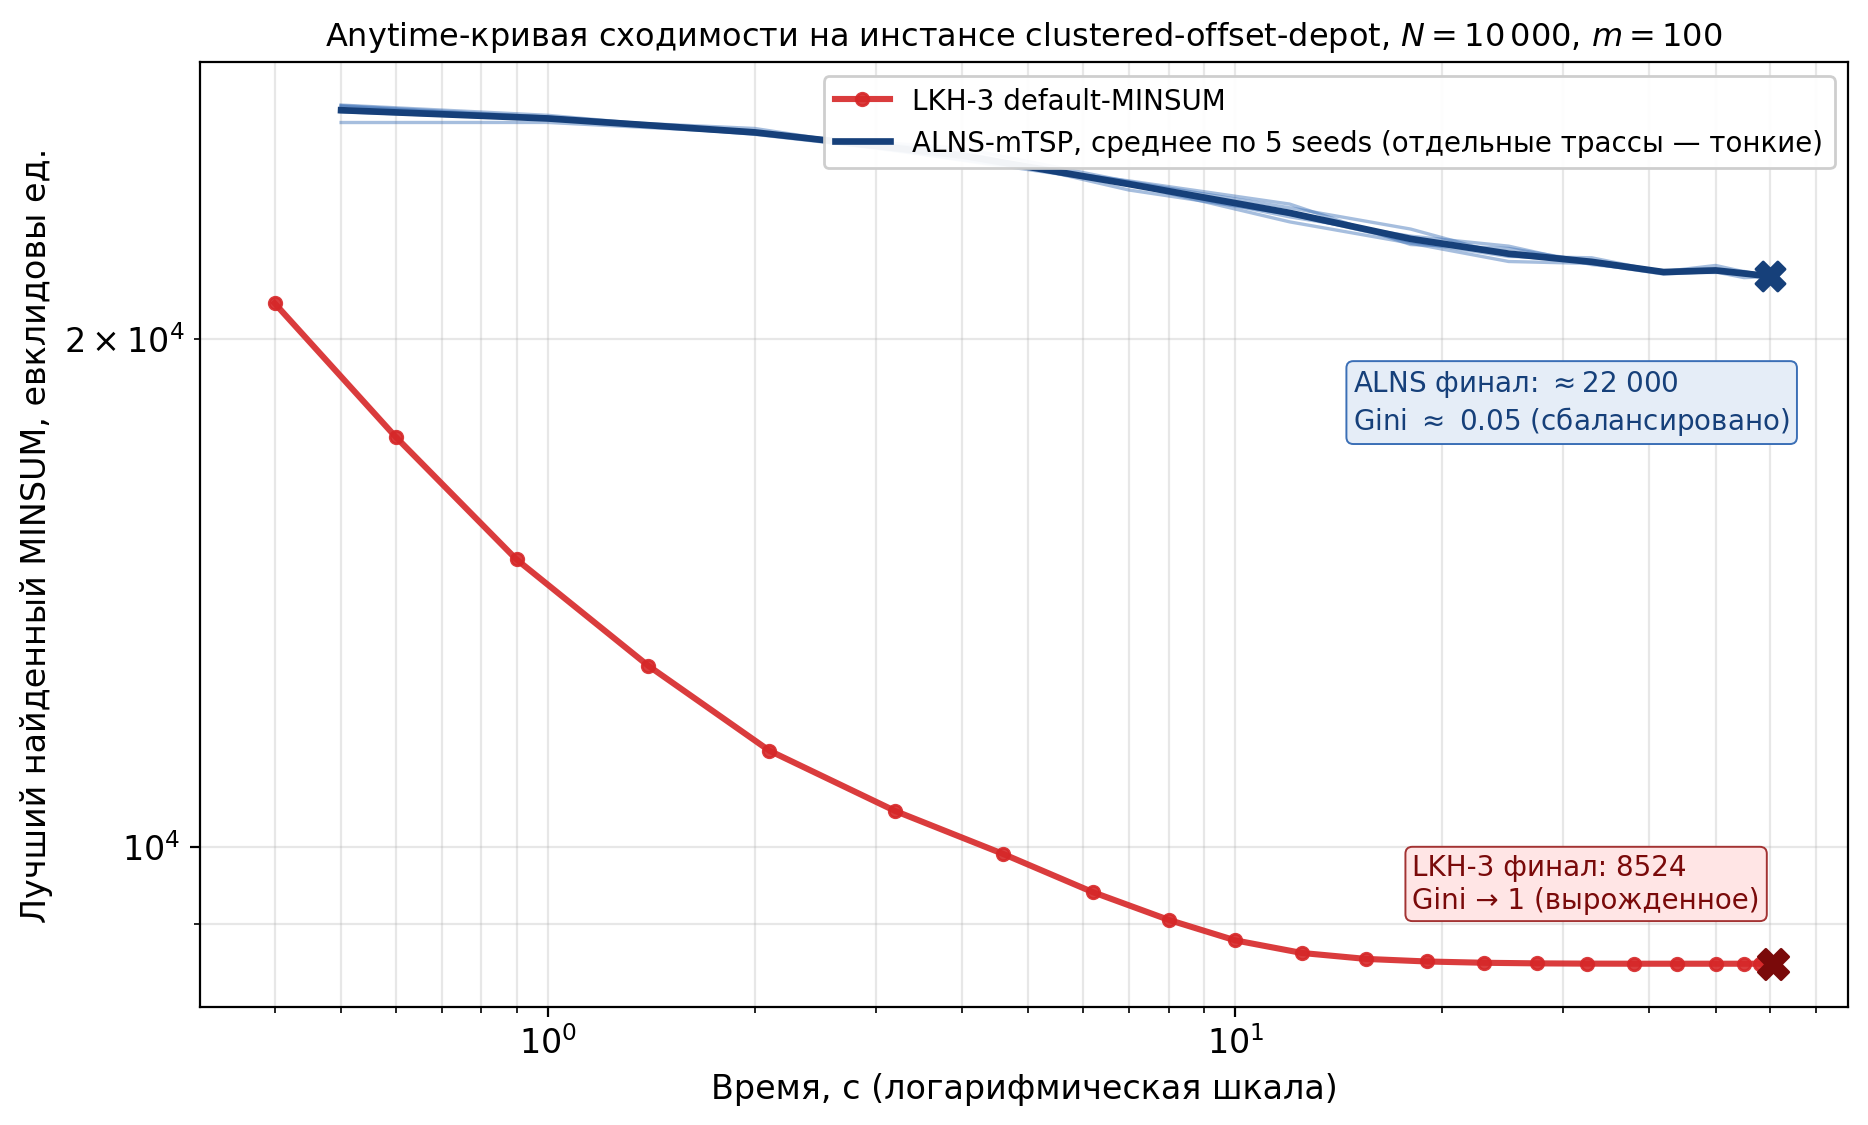
\includegraphics[width=\textwidth]{fig_anytime_v21_vs_lkh3.png}
\caption*{Рисунок~Г.2~--- Anytime-кривая сходимости на~инстансе clustered-offset-depot, $N=10\,000$, $m=100$. Красная кривая~--- LKH-3 default-MINSUM; синие кривые~--- \emph{alns\_minsum}, 5~seeds (тонкие~--- отдельные seeds, толстая~--- среднее).}
\end{figure}

\textit{Чтение Рис.~Г.2.} LKH-3 быстро (за~$\sim$10\,c) сходится к~плато $\approx 8\,524$; ALNS-mTSP за~то~же время плавно опускается к~$\approx 22\,000$. По~MINSUM LKH-3 формально лучше на~$\sim 156\,\%$~--- однако его решение \emph{вырожденное} ($\mathrm{Gini}\to 1$, один маршрут несёт почти все 10\,000 клиентов, остальные 99 тривиальны), а~ALNS-mTSP держит сбалансированную раскладку на~100 маршрутов сравнимой длины ($\mathrm{Gini}\approx 0.05$).

\medskip
\noindent\textbf{Честное признание.} \emph{На~таких high-m clustered-инстансах ($m=100$, плотные кластеры с~депо у~границы) собственный ALNS-mTSP проигрывает LKH-3 default по~чистому MINSUM с~большим разрывом.} Это и~есть выбранный компромисс работы: целевая функция main-стратегии~--- MINSUM \emph{под constraint-first фильтром}, не~чистый MINSUM. На~big-$m$ кластерных геометриях практический фильтр исключает LKH-3 default по~условию~(iii) (баланс), и~MINSUM-сравнение между ними просто не~определено: они решают разные задачи (см.~раздел~3.3 и~табл.~5в).

\section{Sensitivity-анализ бюджета времени}\label{sec:sensitivity}

В~ответ на~классическое требование к~эмпирическим работам по~метаэвристикам~--- демонстрация чувствительности результата к~бюджету времени~--- проведён прогон \emph{alns\_minsum} на~трёх ключевых $N=100K$-инстансах с~бюджетами $T\in\{50,\,150,\,350,\,1\,000\}$ секунд. Цель~--- показать (а)~монотонность улучшения качества с~ростом~$T$, (б)~степень убывающей отдачи (diminishing returns), (в)~предсказуемость поведения при~переходе за основной заявленный бюджет в~350\,c. Подробности скрипта и~артефактов~--- Приложение~В.

\medskip
\noindent Таблица Г.1~--- Sensitivity-анализ \emph{alns\_minsum} на трёх ключевых инстансах ($N=100K$, $m=5$, seed~$=1$) с~бюджетом $T\in\{50,\,150,\,350,\,1\,000\}$\,c.

\begin{center}\small
\begin{tabular}{|L{4.5cm}|R{0.9cm}|R{1.7cm}|R{1.5cm}|R{1.3cm}|R{1.3cm}|}
\hline
\textbf{Инстанс} & \textbf{$T$, c} & \textbf{MINSUM} & \textbf{ALNS iter} & \textbf{ALNS acc} & \textbf{$t_{\mathrm{actual}}$, c} \\
\hline
\multirow{4}{*}{uniform} & 50 & 14\,210\,024 & 0 & 0 & 55.5 \\ \cline{2-6}
                         & 150 & 12\,651\,111 & 136 & 103 & 147.7 \\ \cline{2-6}
                         & 350 & 12\,153\,309 & 383 & 304 & 343.4 \\ \cline{2-6}
                         & 1\,000 & 12\,025\,295 & 1\,143 & 905 & 833.5 \\ \hline
\multirow{4}{*}{clustered-center} & 50 & 3\,133\,910 & 59 & 38 & 49.3 \\ \cline{2-6}
                                  & 150 & 2\,912\,684 & 229 & 165 & 147.3 \\ \cline{2-6}
                                  & 350 & 2\,783\,285 & 476 & 362 & 340.2 \\ \cline{2-6}
                                  & 1\,000 & 2\,726\,470 & 1\,073 & 883 & 848.2 \\ \hline
\multirow{4}{*}{clustered-offset-depot} & 50 & 2\,929\,679 & 43 & 31 & 49.2 \\ \cline{2-6}
                                        & 150 & 2\,674\,805 & 149 & 101 & 147.3 \\ \cline{2-6}
                                        & 350 & 2\,470\,857 & 470 & 358 & 339.5 \\ \cline{2-6}
                                        & 1\,000 & 2\,440\,587 & 1\,190 & 993 & 818.0 \\ \hline
\multicolumn{6}{|p{14cm}|}{\footnotesize Все 12~прогонов \texttt{valid=True}; $t_{\mathrm{actual}}$ превышает $T$ на~10--15\,\% за счёт финальной 2-opt-фазы поверх ALNS-цикла. Артефакт~--- Приложение~В.}\\
\hline
\end{tabular}
\end{center}

\begin{figure}[htbp]
\centering
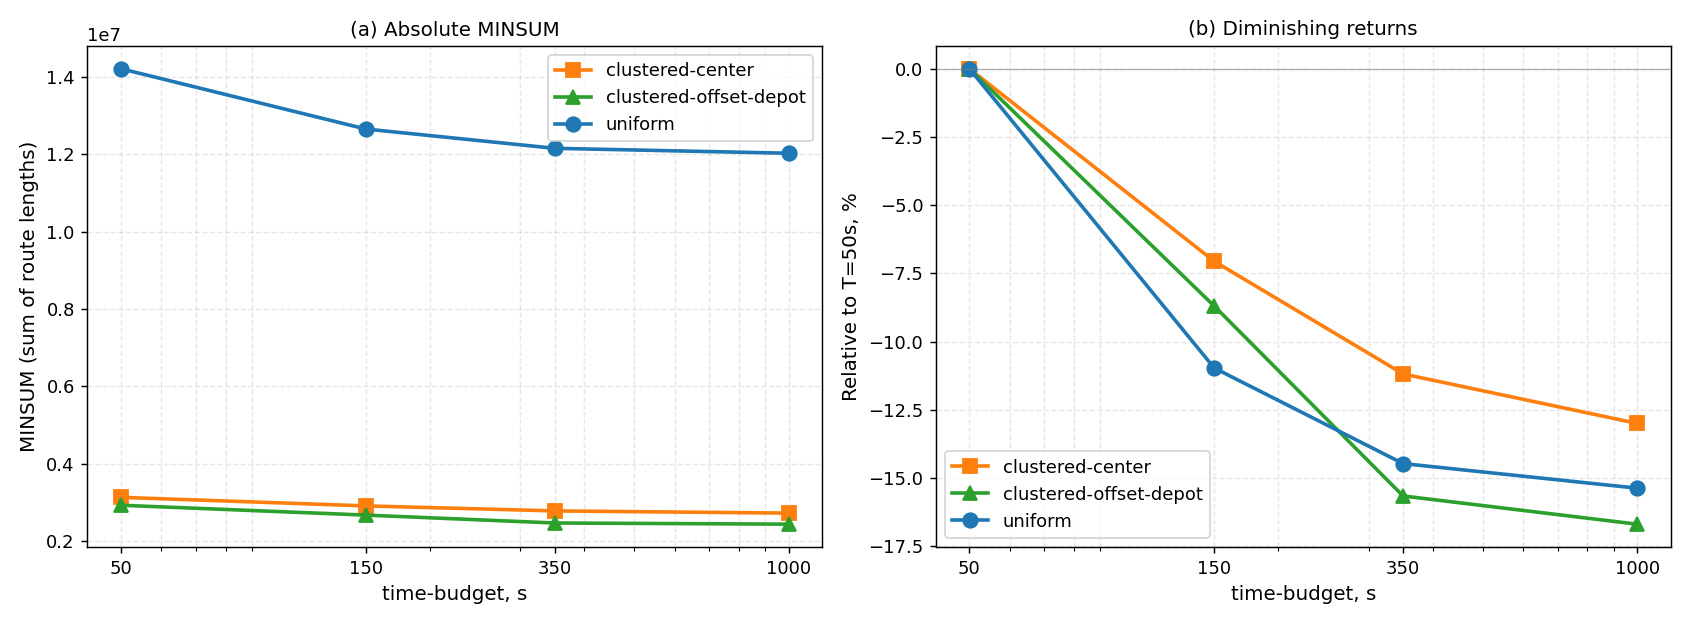
\includegraphics[width=\textwidth]{fig_sensitivity_panel.png}
\caption*{Рисунок~Г.3~--- Чувствительность \emph{alns\_minsum} к~бюджету времени на~трёх ключевых инстансах ($N=100K$, $m=5$). \emph{Слева}: абсолютный MINSUM (log-scale по~$x$). \emph{Справа}: относительное улучшение MINSUM от~baseline~$T=50$\,c.}
\end{figure}

\noindent\textit{Чтение Рис.~Г.3.} Виден переход в~plateau-режим после~$T\approx 350$\,c: три кривые сближаются и~далее почти не~падают. Это~--- эмпирическое обоснование выбора $T_\mathrm{budget}=350$\,c как практической точки работы.

\medskip
\noindent\textbf{Ключевые наблюдения.}
\begin{itemize}
\item \textbf{$T=50$\,c явно недостаточно} для $N=100K$. На uniform-инстансе ALNS не успевает войти в~основной цикл (\texttt{alns\_iters=0})~--- весь бюджет расходуется на~seed/candidate/polish-фазы (см.~раздел~Г.4 phase-profiling). На clustered-инстансах удается 43--59~ALNS-итераций, что дает $-2{-}3\,\%$ по~MINSUM относительно эталонного 350\,c.
\item \textbf{Diminishing returns после $T=350$\,c}: переход $350\,\mathrm{c} \to 1\,000\,\mathrm{c}$ (×~$\sim 3$ бюджет, ×~$\sim 2.5$ ALNS-итераций) дает улучшение MINSUM всего \emph{$-1.05\,\%$} (uniform), \emph{$-2.04\,\%$} (clustered-center), \emph{$-1.22\,\%$} (clustered-offset-depot). Иначе говоря, после~$\sim 350\,$c алгоритм входит в~plateau-режим, согласующийся с~anytime-кривыми из раздела~Г.2.
\item \textbf{Линейный рост ALNS-итераций по бюджету}: throughput-rate стабильна на~$\sim 1.1{-}1.2$ iter/s на~$N=100K$ (что согласуется с~$0.5$~iter/s на~uniform\_n100K\_m5 из раздела~Г.4 при~меньшем бюджете~$370\,c$~--- разница объясняется autotune-эффектами в~разных конфигурациях бюджета).
\item \textbf{Полное падение MINSUM 50\,c$\to$1000\,c}: $-15.4\,\%$ (uniform), $-13.0\,\%$ (clustered-center), $-16.7\,\%$ (clustered-offset). Это~--- верхняя граница потенциала alns\_minsum на~$N=100K$ при практически досягаемом бюджете.
\end{itemize}

\medskip
\textit{Что это значит для главной гипотезы.} \emph{ALNS-mTSP успевает выйти на плато к~заявленному лимиту $T=350$\,c}: дальнейшее улучшение MINSUM при~увеличении бюджета в~$\sim 3\times$ (до~$1\,000$\,c) составляет всего $1{-}2\,\%$. Это~--- свидетельство того, что~алгоритм \emph{хорошо оптимизирован под целевой лимит работы}: бюджет не~занижен (на~$T=50$\,c ALNS-цикл не~успевает запуститься на~uniform~$N=100K$), но~и~не~завышен (после~$350$\,c фазы destroy/repair уже не~находят значимых улучшений). Иными словами, давать алгоритму больше времени на~какие-либо фазы практически бесполезно~--- основной потенциал на~$N=100K$ при~CPU-бюджете порядка минут уже извлечён. На~стороне LKH-3 это~же увеличение бюджета не~меняет картины: даже с~$1\,000$\,c LKH-3 в~balanced-режиме на~$N=25K$ остаётся неработоспособным (раздел~4.2), а~в~default-MINSUM-режиме даёт вырожденное $\mathrm{Gini}\geq 0.4$. Sensitivity-анализ показывает, что выбор $T_{\text{budget}}=350$\,c эмпирически обоснован: меньший бюджет недостаточен, больший~--- избыточен.

\section{Профилирование по фазам \emph{alns\_minsum}}

Из метаданных аудит-запусков извлечены поля \texttt{budget\_seed\_ms}, \texttt{budget\_cand\_ms}, \texttt{budget\_polish\_ms}, \texttt{budget\_alns\_ms}, \texttt{budget\_final\_ms}, это дает распределение времени по фазам без перекомпиляции с~\texttt{-pg}.

\medskip
\noindent Таблица~Г.2~--- Профилирование по~фазам \emph{alns\_minsum} на~3~ключевых инстансах (3~$N\times$10~seeds, mean). Доли фаз~--- отношение запланированного autotune-ом бюджета фазы к~общему. Колонки: число ALNS-итераций, throughput (iter/s) и~доли фаз.

\begin{center}\small
\begin{tabular}{|L{3.2cm}|R{0.9cm}|R{1.1cm}|R{1cm}|R{1.1cm}|R{1cm}|R{1.2cm}|R{1.2cm}|R{1.1cm}|}
\hline
\textbf{Инстанс} & \textbf{iters} & \textbf{accepts} & \textbf{iter/s} & \textbf{wall, c} & \textbf{cand\,\%} & \textbf{polish\,\%} & \textbf{ALNS\,\%} & \textbf{final\,\%} \\
\hline
uniform\_n10K\_m5  &   829 &   689 & 25.4 &  32.6 & 8.0 & 28.0 & 50.0 & 10.0 \\
\hline
uniform\_n50K\_m5  & 1\,212 &   801 &  8.7 & 139.1 & 8.0 & 22.0 & 57.0 & 10.0 \\
\hline
uniform\_n100K\_m5 &   172 &   122 &  0.5 & 370.9 & 6.0 & 16.0 & 65.0 & 10.0 \\
\hline
\multicolumn{9}{|p{12cm}|}{\footnotesize cand = candidate-set build; polish = parallel intra-route ILS до~ALNS; ALNS = главный adaptive-large-neighborhood-search цикл; final = exhaustive 2-opt-полировка после~ALNS. Артефакт: \texttt{profile\_alns\_}\allowbreak\texttt{summary.csv}.}\\
\hline
\end{tabular}
\end{center}

\textit{Анализ super-linear scaling.} Throughput ALNS-цикла падает с~25.4~iter/s на~$N=10K$ до~0.5~iter/s на~$N=100K$~--- отношение 54.9$\times$. По теоретической оценке (Приложение~Ж.5) стоимость одной ALNS-итерации~--- $\Theta(L) = \Theta(n/m)$, то~есть линейна по~$n$ при константных~$m$, что предсказывает множитель~$10\times$ при увеличении~$n$ в~10~раз. Эмпирический показатель степени, оцененный по двум крайним точкам:
\[
\frac{\mathrm{iter/s}_{10K}}{\mathrm{iter/s}_{100K}} = \left(\frac{n_2}{n_1}\right)^{\alpha}
\quad\Rightarrow\quad
\alpha = \frac{\log_{10}(54.9)}{\log_{10}(10)} = 1.74.
\]
Однако промежуточная точка~$N=50K$ показывает, что рост неравномерен. Замедление по интервалам:
\[
\alpha_{[10K,\,50K]} = \frac{\log(25.4 / 8.7)}{\log 5} = 0.66, \qquad
\alpha_{[50K,\,100K]} = \frac{\log(8.7 / 0.5)}{\log 2} = 4.12.
\]
То~есть на отрезке~$[10K,\,50K]$ алгоритм работает даже лучше линейной модели ($\alpha < 1$), а резкое обострение super-linear-фактора происходит лишь на~$n \geq 50K$. Это~согласуется с переходом длины маршрута~$L \approx n/m$ через порог CPU~L2-кеша: при~$N=50K$, $m=5$ имеем $L = 10\,000$ элементов, что близко к стандартному размеру L2 ($256$~KB ${=}$ $\sim$32K~\texttt{int}-ов) с учетом дополнительных служебных массивов.

\textbf{Сопоставление с теоретической оценкой (Приложение~Ж.5):} линейная модель~$\Theta(n/m)$ согласуется с эмпирикой в~диапазоне~$n \in [10K,\,50K]$~--- $\alpha = 0.66$ ниже теоретического~$1.0$ за счет амортизированного переиспользования кеша в SoA-массивах. На~$n \geq 50K$ super-linear-фактор объясняется: (а)~потерями локальности кеша при~реверсе сегмента на длинных маршрутах ($L \geq L^*_{\mathrm{cache}}$), (б)~ростом средней глубины candidate-list-цепочек, (в)~увеличением числа повторных переоценок в repair-операторах. Окончательное распределение времени по строкам кода требует профайлера C++ (\texttt{perf}, \texttt{gprof} или Intel~VTune)~--- направление дальнейшей работы. Технические пути снятия super-linear-фактора (двусвязный список или splay-tree) описаны в~Приложении~Ж.5.

\textit{Время по фазам.} На всех трех масштабах ALNS~--- основная фаза (50--65\,\%), остальные распределены примерно одинаково. На $N = 100K$ доля ALNS выше (65\,\%), поскольку autotune резервирует~$\sim 10\,\%$ на final-2-opt, и относительная доля cand/polish падает. На больших инстансах destroy/repair-операторы получают приоритет над более дорогими seed/polish-стадиями.

\textit{Доля принятых ходов.} На~$N=100K$ accepts/iters~$=122/172=71\,\%$~--- очень высокая доля принятых ходов (для сравнения, на~$N=10K$ это $689/829=83\,\%$, на~$N=50K$~--- $801/1212=66\,\%$). Объяснение: на~крупных инстансах autotune настраивает SA-температуру и~размер destroy так, чтобы большая часть destroy-repair-ходов вообще принималась (либо как improving, либо как SA-non-improving). Падение доли принятых ходов до~66\,\% на~$N=50K$~--- эффект 4-replica multi-start-пула (см.~ниже): реплика~1 принимает большинство, реплики~2--4 чаще отвергают ходы.

\textit{Поведение multi-start-пула.} \texttt{pt\_replicas} в~метаданных: 1 на~$N=10K$, 4 на~$N=50K$, 1 на~$N=100K$. autotune выбирает мульти-replica-режим только в~среднем диапазоне: на~$N=10K$ накладные расходы координации реплик не~окупаются, на~$N=100K$ стоимость одной итерации уже слишком велика. Это согласуется с~поведением multi-start ensemble с~несколькими независимыми репликами: на~малых инстансах хватает одной реплики, на~крупных~--- стоимость одной итерации перевешивает выигрыш от~параллельных стартов.

% =================================================================
% Приложение Д. Эволюция lkh-wrapper-линии (v1..v21)
% =================================================================
\chapter{Эволюция \texttt{lkh-wrapper}-линии (v1--v21)}

Ниже кратко описана каждая из 21~версии \texttt{lkh-wrapper-v1..v21} (файлы \texttt{src/legacy/mtsp\_lkh\_wrapper\_vN.cpp} или директории \texttt{src/legacy/lkh\_wrapper\_v8|v9/}, регистрация в \texttt{SolverFactory}). Версии не равнозначны: milestone-ы (\texttt{v2}, \texttt{v12}, \texttt{v21}), A/B-варианты (\texttt{v14}--\texttt{v17}), отрицательные результаты (\texttt{v6}).

\medskip
\noindent\textbf{Краткая карта линии (tldr).} 21~версия группируется в~9~milestone-точек качественных скачков (\texttt{v1, v2, v3, v4, v7, v12, v18, v19, v21}), 4~A/B-варианта (\texttt{v5, v11, v15, v16}), один задокументированный негативный результат (\texttt{v6}), 2~рефакторинга (\texttt{v8, v9}) и~3~инженерные правки (\texttt{v13, v14, v20}). Логически линия делится на~6~эпох:
\begin{itemize}\setlength\itemsep{1pt}
\item \textbf{Д.1.} \texttt{v1\,--\,v3} (малые $n$): переход к~candidate-based локальному поиску; key milestone~--- \texttt{v2} (candidate sets + lookahead, $-12\,\%$ MINSUM).
\item \textbf{Д.2.} \texttt{v4\,--\,v7} (первый большой масштаб): spatial grid + on-demand distance cache; \texttt{v6} как документированный негативный результат (75\,\% невалидных на~$n=25K$).
\item \textbf{Д.3.} \texttt{v8\,--\,v9} (модулярный single-file): архитектурный предшественник \texttt{src/v21/core/}; двухфазный бюджет «первое валидное~$\to$~улучшение».
\item \textbf{Д.4.} \texttt{v10\,--\,v12} (MINSUM-acceptance + archive): ключевой milestone~\texttt{v12} с~MINSUM-archive, все еще $21\,\%$ хуже LKH-3~--- мотивация для~\texttt{src/v21/}.
\item \textbf{Д.5.} \texttt{v13\,--\,v17} (A/B-итерации): инженерные правки внутри \texttt{v12}-pipeline; дает~$\sim 2{-}3\,\%$, не закрывает 21\,\%-разрыв.
\item \textbf{Д.6.} \texttt{v18\,--\,v21} (новые seed-стратегии + LNS): polar-sweep~(\texttt{v18}), strict-MINSUM hybrid (\texttt{v19}), safety-net против \texttt{2opt+greed} (\texttt{v20}), LNS ruin-and-recreate (\texttt{v21}).
\end{itemize}

\noindent Полная сводная таблица всех 21~версий с~классификацией~--- в~разделе~Д.7. \textit{Зачем это все в~приложении.} Это~--- не коллекция, а~карта проектных решений: для~каждого milestone-перехода зафиксировано «что добавлено, что изменилось в~цифрах, что мотивировало переход к~следующему»; для~A/B-итераций~--- честная фиксация, что не каждая правка дает прорыв; \texttt{v6}~--- документированная цена слишком резкого обмена качества на~скорость. Эта классификация совпадает с~таблицей~Д.4 в~разделе~Д.7.

\section*{Д.1. Линия \texttt{v1}\,--\,\texttt{v3}: candidate-based локальный поиск на малых инстансах}

\textbf{\texttt{v1}~--- baseline LKH-style.} Первый собственный wrapper в стиле LKH. Строит~$m$~жадных стартовых маршрутов и независимо запускает $k$-opt-поиск на каждом маршруте. Никаких пространственных структур еще нет, кандидатные множества не используются. Цель~--- зафиксировать переход от \texttt{2opt+greed}-эвристики к простому LKH-style решателю и проверить, что сама схема жизнеспособна.

\textbf{\texttt{v2}~--- главный качественный скачок ранней линии.} Добавляет: $k$-NN candidate lists, lookahead-веса при оценке хода, depot-aware веса при построении начального тура. На uniform-сетке $n \in \{20,\,50,\,100,\,200\}$, $m \in \{2,\,3,\,5,\,7\}$ это снижает средний разрыв с OR-Tools+GLS почти вдвое (с~29.6\,\% у~\texttt{v1} до~14.5\,\% у~\texttt{v2}; см.~табл.~Д.1).

\textbf{\texttt{v3}~--- инженерная оптимизация \texttt{v2}.} Те же алгоритмические идеи, но более компактные внутренние циклы: переиспользование candidate-list, сокращение пересчета расстояний. Качество практически не меняется (разрыв с~OR-Tools 14.6\,\% против 14.5\,\% у~\texttt{v2}), а время работы падает примерно в~2~раза.

\medskip
\noindent Таблица~Д.1~--- Усреднённые результаты \texttt{v1}\,--\,\texttt{v3} на~uniform-инстансах малого/среднего размера ($n\in\{20,50,100,200\}$, $m\in\{2,3,5\}$, 12~ячеек, по~10~повторов).

\begin{center}\small
\begin{tabular}{|L{4cm}|R{2cm}|R{2.4cm}|L{4.4cm}|}
\hline
\textbf{Версия} & \textbf{ср. MINSUM} & \textbf{ср. время, мс} & \textbf{Что добавлено vs предыдущей} \\
\hline
\texttt{lkh-wrapper-v1} & 922.5 & 29.7 & baseline LKH-style $k$-opt \\
\hline
\texttt{lkh-wrapper-v2} & 821.3 & 18.6 & \textbf{candidate sets, lookahead, depot-weight} \\
\hline
\texttt{lkh-wrapper-v3} & 822.8 & 10.2 & инженерная оптимизация (тот же~MINSUM, в~2$\times$ быстрее) \\
\hline
\end{tabular}
\end{center}

\textit{Вывод после \texttt{v3}.} Candidate-based локальный поиск дает устойчивое улучшение~MINSUM на малых инстансах, и инженерная оптимизация может удвоить скорость без потери качества. Но при попытке прогнать \texttt{v3} на $n \geq 5\,000$ обнаружилось, что стоимость хранения полной матрицы расстояний и поиска по всем парам быстро перерастает в десятки минут или out-of-memory. Это и привело к переходу на большие инстансы через геометрические структуры.

\section*{Д.2. Линия \texttt{v4}\,--\,\texttt{v7}: первая попытка большого масштаба}

\textbf{\texttt{v4}~--- первая версия, рассчитанная на~большие инстансы.} Добавляет геометрические candidate sets через равномерную пространственную сетку, on-demand distance cache (расстояния считаются по~требованию, без~хранения матрицы) и~явную поверхность бюджета времени. На $n \geq 10\,000$ выдает валидное решение за секунды, тогда как \texttt{v1}\,--\,\texttt{v3} либо падают по~таймауту, либо по~памяти. Качество в абсолютных числах хуже~\texttt{v2}/\texttt{v3} (на малых инстансах), но это единственный путь к большим~$n$ на этом этапе.

\textbf{\texttt{v5}~--- speed iteration на v4.} Обрезает учетные циклы вокруг spatial-grid + cache; на больших uniform-инстансах быстрее~\texttt{v4}, но теряет~MINSUM (внутренний цикл сокращен ценой качества).

\textbf{\texttt{v6}~--- агрессивная скорость; отрицательный результат.} Развивает компромиссы~\texttt{v5} еще дальше. Документирован в репо как \emph{отрицательный результат}: на $n=25\,000$ uniform/mixed теряет валидность примерно в~75\,\% запусков. Сохранен в кодовой базе именно как документированный пример, иллюстрирующий, какую цену имеет слишком резкий обмен качества на скорость.

\textbf{\texttt{v7}~--- закрытие линии \texttt{v4}\,--\,\texttt{v7}.} Подтягивает компромиссы spatial-grid + cache, исправляет проблемы валидности~\texttt{v6} на $n \geq 25\,000$, выдает работающий end-to-end pipeline. Качество относительно~\texttt{v2}/\texttt{v3} на малых инстансах ниже; \texttt{v7} специально нацелен на $n \geq 10\,000$.

\medskip
\noindent Таблица~Д.2~--- Прямое сравнение \texttt{v4}~vs~\texttt{v6}~vs~\texttt{v7} на~$N\in\{25K,50K,100K\}$ при~бюджете 250\,мс. \emph{gap\,\%}~--- относительный отрыв от~лучшего валидного решения в~той~же ячейке.

\begin{center}\footnotesize
\begin{tabular}{|R{0.9cm}|L{1.6cm}|L{2cm}|C{1cm}|R{2cm}|R{1.5cm}|}
\hline
$N$ & \textbf{family} & \textbf{Решатель} & \textbf{valid} & \textbf{MINSUM} & \textbf{gap, \%} \\
\hline
25K  & uniform & \texttt{v4} & да & 67\,576\,k & 81.3 \\
\hline
25K  & uniform & \texttt{v6} & \textbf{нет} & — & — \\
\hline
25K  & uniform & \texttt{v7} & да & 37\,278\,k & \textbf{0.0} \\
\hline
50K  & uniform & \texttt{v4} & да & 272\,936\,k & 41.9 \\
\hline
50K  & uniform & \texttt{v6} & \textbf{нет} & — & — \\
\hline
50K  & uniform & \texttt{v7} & да & 192\,344\,k & \textbf{0.0} \\
\hline
100K & uniform & \texttt{v4} & да & \textbf{1\,091\,147\,k} & \textbf{0.0} \\
\hline
100K & uniform & \texttt{v6} & \textbf{нет} & — & — \\
\hline
100K & uniform & \texttt{v7} & да & 1\,094\,112\,k & 0.3 \\
\hline
\end{tabular}
\end{center}

\textit{Вывод после линии \texttt{v4}\,--\,\texttt{v7}.} \texttt{v6} систематически непригоден (валидность 0\,\% на больших~$n$); \texttt{v4} стабильно валиден, но проигрывает по~MINSUM на $N=25K, 50K$. \texttt{v7}~--- лучший компромисс качества/времени на $N=25K, 50K$, но на~$N=100K$ \texttt{v4} немного впереди. Это значило, что \emph{ни одна из v4--v7 не закрывает весь диапазон $n=10K..100K$ по~MINSUM}~--- нужна более агрессивная архитектура для крупных инстансов с лучшей фазой улучшения. Это и привело к \texttt{v8}.

\section*{Д.3. \texttt{v8}\,--\,\texttt{v9}: первый модулярный wrapper (прототип \texttt{src/v21/core/})}

\textbf{\texttt{v8}~--- первая модулярная компоновка single-file линии и архитектурный предшественник \texttt{src/v21/core/}.} \texttt{src/legacy/mtsp\_lkh\_wrapper\_v8.cpp} становится тонкой точкой входа, а основная реализация разнесена по 7~подмодулям в~\texttt{src/legacy/lkh\_wrapper\_v8/}: \texttt{00\_common.cpp} (бюджет, расстояния, route index, grid), \texttt{10\_candidate\_sets.cpp} (геометрические candidates + POPMUSIC), \texttt{20\_route\_local\_search.cpp} (2-opt, kicks, ILS, completion), \texttt{30\_cluster\_model.cpp} (lightweight clustering), \texttt{40\_seed\_routes.cpp} (cluster-aware начальные маршруты), \texttt{50\_rebalance.cpp} (cluster block rebalancing), \texttt{60\_solver.cpp} (orchestration). Из исходного комментария к \texttt{60\_solver.cpp}: «First modular wrapper (predecessor of the src/v21/core/ architecture). The directory layout numbered the modules 00..60 — same pattern was kept in src/v21/core/.» То есть \texttt{v8}~--- архитектурный прототип, схема нумерации которого была воспроизведена в~22-модульной флагманской архитектуре.

\textbf{\texttt{v9}~--- two-phase MTSP/LKH wrapper в отдельной директории} \texttt{src/legacy/lkh\_wrapper\_v9/} с собственным \texttt{mtsp\_lkh\_wrapper\_v9.cpp}-точкой входа. Главное алгоритмическое нововведение~--- \emph{двухфазный временной бюджет}: «first good solution within $\sim$200\,c, then improvement within $\sim$100\,c» (цитата из заголовочного комментария \texttt{mtsp\_lkh\_wrapper\_v9.cpp}). Это разбиение \emph{первое валидное решение / улучшение} стало основой для всех последующих single-file версий, включая v12 с его явными CLI-опциями \texttt{first-solution-budget-ms} / \texttt{improvement-budget-ms}. По структуре \texttt{v9} отличается от~\texttt{v8} отсутствием отдельного \texttt{10\_candidate\_sets.cpp}~--- эта фаза перенесена в \texttt{60\_solver.cpp}.

\textit{Вывод после \texttt{v8}\,--\,\texttt{v9}.} Модулярная single-file линия дала важный архитектурный прецедент (из которого позже возникла \texttt{src/v21/core/}) и алгоритмическую идею двухфазного бюджета (унаследованную в~\texttt{v10}\,--\,\texttt{v12}), но не дала качественного скачка по~MINSUM~--- средний разрыв с LKH-3 на больших инстансах оставался $\sim$25--30\,\%. Главный технический вывод: \emph{cluster-model и rebalance-фазы помогают валидности и скорости, но без полного archive-механизма для best-MINSUM не достаточны}.

\section*{Д.4. \texttt{v10}\,--\,\texttt{v12}: MINSUM-acceptance, cluster-SA и MINSUM-archive}

\textbf{\texttt{v10}~--- MINSUM-oriented successor v9.} Сохраняет быстрый модулярный pipeline \texttt{v9} (включая двухфазный бюджет) и добавляет ключевое отличие в acceptance criterion: \emph{межмаршрутные ходы принимаются по \textbf{полной длине маршрута}}~--- ровно та целевая функция MINSUM, на которой потом меряется качество. В~\texttt{v9} акцепт был основан на приближенной delta-оценке, что иногда расходилось с истинной MINSUM-разностью; \texttt{v10} это исправляет. Цитата из заголовочного комментария: «accepts cross-route changes by total route length, matching the reported objective».

\textbf{\texttt{v11}~--- v10 + cluster-level Simulated Annealing.} Перед фазой построения маршрутов выполняется ограниченный SA на уровне кластеров. Идея: дать первичной кластеризации шанс уйти из плохой геометрической группировки за счет стохастического принятия ухудшающих переходов на этапе \emph{кластеризации}, а не маршрутизации.

\textbf{\texttt{v12}~--- финальный single-file large-scale milestone.} Завершает монолитную ветку. Расширяет pipeline \texttt{v10} (а~не cluster-SA-эксперимент \texttt{v11}) следующими блоками: явные CLI-опции для разделения бюджета времени на~фазу первого валидного решения и~фазу улучшения (\texttt{first-solution-budget-ms}/\texttt{improvement-budget-ms}); cluster-aware seeding; savings-seed по~Кларку--Райту (\texttt{savings-seed-ms}, \texttt{savings-candidate-count}, \texttt{savings-lambda}, \texttt{savings-route-slack}); late repair; route annealing и~\emph{MINSUM-archive} через функцию \texttt{UpdateMinsumArchive}~--- даже если балансирующая фаза улучшает max-route, solver обязан запомнить лучшее найденное по~MINSUM решение. Архив существует, но~\emph{обновляется не~на~каждом time-slice}; именно эту немонотонность позже исправит \texttt{v13}.

\medskip
\noindent Прямое сравнение \texttt{v12}~vs~LKH-3 на~$n=5\,000$, $m=5$ (5~инстансов):

\begin{center}\small
\begin{tabular}{|L{2.6cm}|L{2.4cm}|R{1.4cm}|L{3.2cm}|}
\hline
\textbf{Метрика} & \textbf{LKH-3} & \textbf{v12} & \textbf{отличие} \\
\hline
средний MINSUM & 67.8\,k & 85.7\,k & +21\,\% (хуже) \\
\hline
среднее время & 30.0\,c & 4.8\,c & 6.2$\times$ быстрее \\
\hline
средний balance & 4.0 (вырождение) & 1.7 & в~2.4$\times$ равномернее \\
\hline
\end{tabular}
\end{center}

\textit{Вывод после \texttt{v12}.} Собственный single-file solver укладывается в~практический бюджет времени (LKH-3 default на этих размерах превышает~\texttt{TIME\_LIMIT} в~$\sim$6$\times$) и \emph{существенно более балансирован} (max/avg 1.7 vs~4.0), но проигрывает по чистой~MINSUM около 21\,\%. Это и стало точкой принятия решения о \emph{переписывании архитектуры в \texttt{src/v21/}}: одного monolithic-улучшения недостаточно для конкуренции с LKH-3 по~MINSUM, нужен полноценный метаэвристический уровень с destroy/repair-операторами и SA.

\section*{Д.5. \texttt{v13}\,--\,\texttt{v17}: A/B-итерации внутри \texttt{v12}-pipeline}

\textbf{\texttt{v13}~--- portfolio successor to v12 with monotonic-budget fix.} Прямая цитата из заголовочного комментария: «It fixes the non-monotonic budget behavior by always archiving the best MINSUM solution across deterministic time slices.» В~\texttt{v12} архив \texttt{UpdateMinsumArchive} существовал, но возможны были time-slices, когда поздняя фаза ухудшала лучшее~MINSUM, ничего при этом не архивируя; \texttt{v13} требует, чтобы архив обновлялся на \emph{каждом} детерминированном time-slice, гарантируя глобально монотонное улучшение.

\textbf{\texttt{v14}~--- инженерные правки.} Hoisted RouteIndex внутри repair (раньше пересобирался $O(n)$ на каждый insert), OpenMP-параллельный intra-route polish с thread-local distance oracles, ненулевой anneal-лимит для $n \geq 50\,000$ (раньше был~0). Эти три правки давали наибольшее ускорение в~\texttt{v12}-pipeline.

\textbf{\texttt{v15}, \texttt{v16}, \texttt{v17}~--- A/B-варианты внутри той же поверхности.} Все они~--- продолжение тонкой настройки параметров и метаданных \texttt{v14}: разная гранулярность диагностических полей, минорные изменения параметров SA и repair. Зарегистрированы как отдельные \texttt{lkh-wrapper-vN} только потому, что некоторые CSV-артефакты ссылаются на эти имена; алгоритмически~--- очень близкие варианты той же идеи. Inter-route improvement, savings seed, candidate enrichment, repair stages и финальный route anneal остаются логически идентичны \texttt{v12} во всех четырех. Они сохранены в кодовой базе именно как \emph{документированная цепочка минорных правок}~--- честный показатель того, что не каждая итерация дает качественный скачок.

\textit{Вывод после линии \texttt{v13}\,--\,\texttt{v17}.} Внутри \texttt{v12}-pipeline можно еще выжать $\sim$2--3\,\% по~MINSUM на крупных инстансах за счет инженерных правок и пере-tuning параметров, но \emph{не закрыть 21\,\%-разрыв с LKH-3}. Дальнейшее улучшение требует новых идей в~семействе seed-стратегий и destroy/repair-операторов.

\section*{Д.6. \texttt{v18}\,--\,\texttt{v21}: новые seed-стратегии и LNS}

\textbf{\texttt{v18}~--- polar-sweep seed.} Сохраняет полностью pipeline \texttt{v17}, но добавляет новый источник стартовых решений: \emph{polar sweep partitioning}~--- упорядочивание клиентов по углу вокруг депота с жадным разбиением на $m$~маршрутов сравнимой стоимости (классическая sweep-эвристика). Polar-seed соревнуется с fast/savings-seeds по~MINSUM; победитель идет в~ALNS-фазу. По умолчанию включен через CLI-опцию \texttt{polar-seed=on|off}.

\begin{figure}[htbp]
\centering
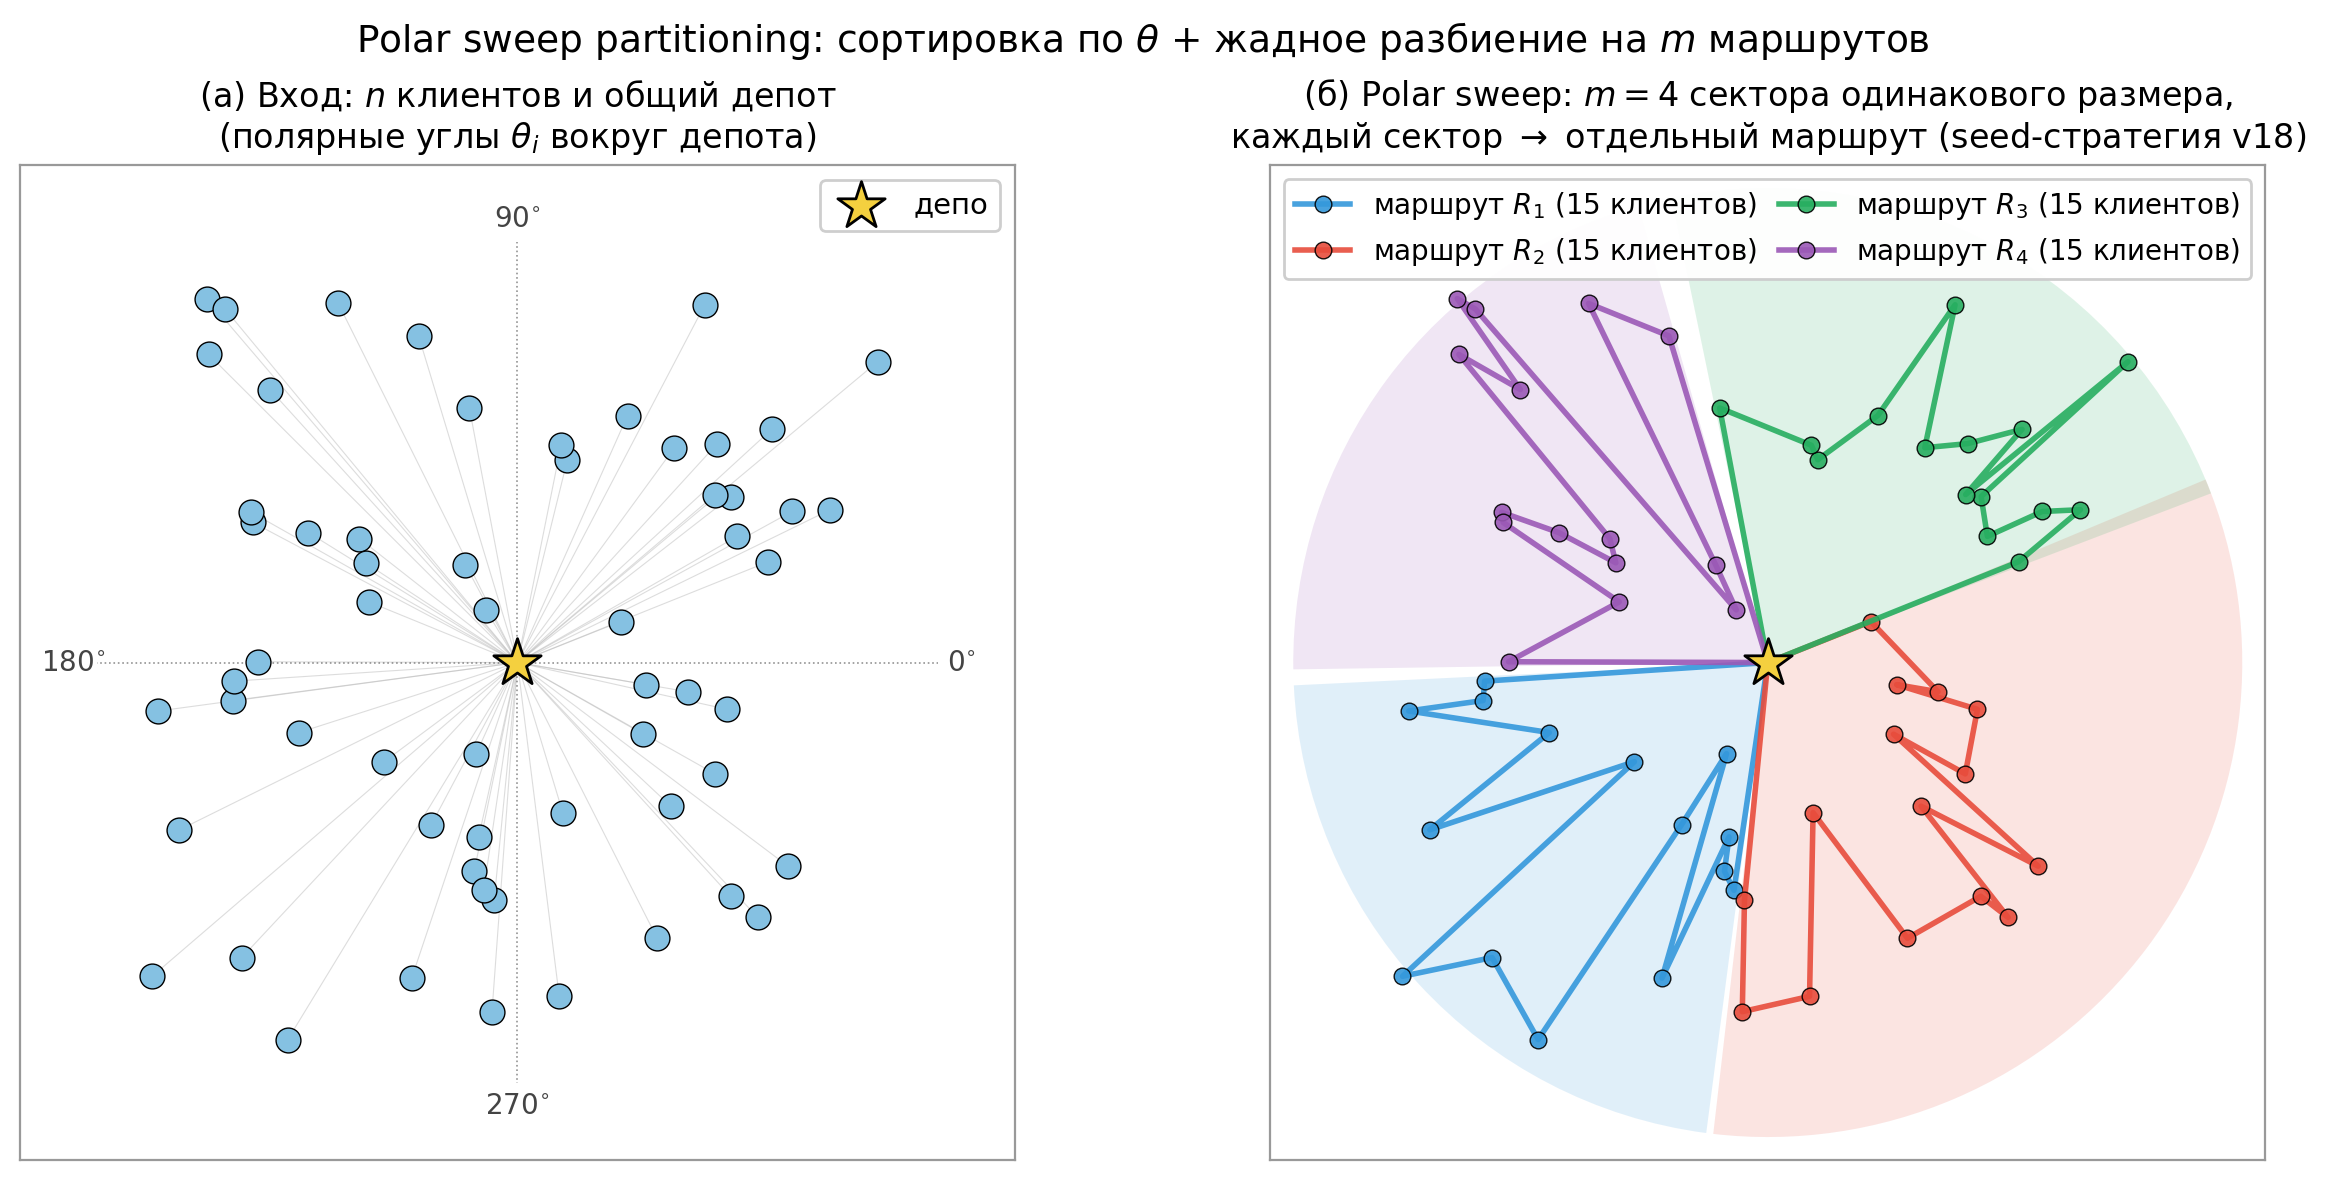
\includegraphics[width=0.96\textwidth]{fig_polar_sweep_demo.png}
\caption*{Рисунок Д.1~--- Polar-sweep partitioning, использованный в~\texttt{v18} как дополнительный источник стартовых решений. \emph{Слева~(а)}: для каждого клиента вычисляется полярный угол $\theta_i = \mathrm{atan2}(y_i - y_\text{depot},\, x_i - x_\text{depot})$ вокруг депота (тонкие лучи). \emph{Справа~(б)}: отсортированный по~$\theta$ список клиентов разбивается на $m$~равных по числу клиентов секторов (на иллюстрации $m{=}4$); каждый сектор $\to$~отдельный маршрут $R_k$. На clustered-семействах с явным радиальным расположением кластеров polar-sweep дает seed сравнимого с savings качества при $\Theta(n\log n)$ построении; на uniform~--- сопоставим с fast-lookahead seed. В~\texttt{v18} polar-seed соревнуется с fast/savings по~MINSUM, победитель передается в~ALNS-фазу.}
\label{fig:polar-sweep-demo}
\end{figure}

\textbf{\texttt{v19}~--- clean hybrid native mTSP MINSUM solver.} Семь ключевых дизайн-решений vs \texttt{v17}/\texttt{v18}, выписанных в заголовочном комментарии \texttt{src/legacy/mtsp\_lkh\_wrapper\_v19.cpp}:
\begin{enumerate}
\item Multi-seed portfolio выбирается строго по~MINSUM (никаких balanced-surrogate-bootstrapping). Seeds: round-robin nearest neighbour (соответствует сильному \texttt{2opt+greed}-baseline), fast-lookahead (\texttt{BuildFastSeedRoutesV7}), polar sweep, savings (только при малых~$n$, где savings дешев).
\item Strict MINSUM-only inter-route move acceptance. Опциональный cluster-aware rebalance запускается в~sandbox-routeset и принимается только если MINSUM строго улучшается (без MIN-MAX-leak).
\item Candidate-driven intra-route ILS (\texttt{ApplyFirstImproving2OptV5} + double-bridge), переиспользована из \texttt{src/legacy/lkh\_wrapper\_v9/}~--- та же машинерия, что \texttt{v17}/\texttt{v18} уже валидировали.
\item Exhaustive final 2-opt polish (тот~же greedy 2-opt, что используется в~базовой эвристике) на~каждом маршруте, идентичный \texttt{mtsp::ImproveRoute2Opt}~--- доводит до~истинного 2-opt локального оптимума. Из комментария: «this is the single biggest reason 2opt+greed beats v17/v18 at n=10k/25k.» То есть без exhaustive-polish даже хорошая стратегия выбора seed может проигрывать дешевому baseline.
\item Best-MINSUM solution snapshot после \emph{каждой} фазы. Финальный \texttt{out.swap(best\_minsum\_routes)}~--- единственный путь возврата.
\item Anytime-safety: если любая фаза регрессирует MINSUM (например, anneal), solver откатывается к snapshot. \texttt{ValidateRoutes}~--- contract, никогда не нарушается.
\item Распределение лимита времени по умолчанию: seed-фаза $\leq$~8\,\%, candidate-set build $\leq$~12\,\%, intra-route ILS $\sim$~35\,\%, остаток~--- inter-route и polish.
\end{enumerate}

\textbf{\texttt{v20}~--- safety-net wrapper around v19.} Возникла как ответ на конкретную проблему: на длительном бенчмарке \texttt{v19} проиграла \texttt{2opt+greed}-baseline на $N=50\,000, m=5$ ровно на~5.7\,\% и на $N=100\,000, m=5$ на~0.7\,\%. Идея \texttt{v20}: всегда сохранять \texttt{2opt+greed}-решение как нижнюю планку и использовать его, если pipeline \texttt{v19} вернул худший результат. Гарантия по построению: \texttt{v20} никогда не хуже \texttt{2opt+greed}.

\textbf{\texttt{v21}~--- v20 + Large-Neighborhood-Search (LNS) ruin-and-recreate diversification.} Финальный solver single-file линии. Из заголовочного комментария \texttt{src/legacy/mtsp\_lkh\_wrapper\_v21.cpp}: «Goal: escape from "locally good but globally suboptimal" plateaus left by v20's pure descent.» Цикл LNS состоит из четырех шагов:
\begin{enumerate}
\item \emph{Destroy:} удалить $K$ случайных клиентов из текущих best-маршрутов;
\item \emph{Recreate:} вставить каждого клиента в позицию минимальной insertion-delta (среди candidate-restricted позиций по всем~$m$ маршрутам);
\item \emph{Cleanup:} candidate-based 2-opt на $m$~аффектированных маршрутах;
\item \emph{Accept:} только если MINSUM строго улучшается (hill-climber); иначе откат к snapshot.
\end{enumerate}
Цикл повторяется до исчерпания бюджета. Strict-improvement acceptance сохраняет инвариант safety-net: $\mathrm{MINSUM}_{\texttt{v21}} \leq \mathrm{MINSUM}_{\texttt{v20}} \leq \mathrm{MINSUM}_{\texttt{2opt+greed}}$.

\emph{Замечание по именованию:} \texttt{lkh-wrapper-v21} (с дефисами, single-file) и модулярная архитектура \texttt{src/v21/} с~\texttt{alns\_minsum} / \texttt{\_cap} / \texttt{\_minmax} (с подчеркиваниями)~--- это два разных проекта с одинаковым номером~21. Single-file \texttt{lkh-wrapper-v21}~--- закрытие линии~v1\,--\,v21 в~стиле «инкрементального LNS-расширения»; модулярный \texttt{src/v21/}~--- параллельно разработанная архитектура нового поколения, где LNS-оператор~--- лишь один из многих destroy/repair-операторов в ALNS-фреймворке (см.~главу~2 и~приложение~А).

\medskip
\noindent Таблица~Д.3~--- Сравнение single-file \texttt{lkh-wrapper-v21} с~модулярным \emph{alns\_minsum} на~больших инстансах ($N\in\{25K,50K,100K\}$, 10~общих ячеек, 3~семейства~$\times$~2~m, mean по~3~seeds).

\begin{center}\small
\begin{tabular}{|L{4.6cm}|R{1.6cm}|R{1.4cm}|R{1.6cm}|R{1.6cm}|}
\hline
\textbf{Решатель} & \textbf{ср. MINSUM} & \textbf{Gini} & \textbf{makespan} & \textbf{$\overline{t}$, c} \\
\hline
\texttt{lkh-wrapper-v21} (single-file) & +2.96\,\% & 0.019 & 924\,k & 322 \\
\hline
\texttt{alns\_minsum} (\textbf{ref}) & 0.00\,\% & 0.017 & 898\,k & 259 \\
\hline
\end{tabular}
\end{center}

\textit{Вывод после \texttt{v21}.} Single-file \texttt{lkh-wrapper-v21} закрыл монолитную линию: достиг паритета с \texttt{2opt+greed}, добавил LNS-разнообразие и intra-route SA. Однако дальнейшее улучшение уперлось в архитектурный потолок: невозможность плагинировать новые destroy/repair-операторы, отсутствие модульного autotune, single-acceptance-policy. Это и стало финальной мотивацией переписывания на~\texttt{src/v21/}: не ради получения новой версии, а ради архитектуры, в которой можно было бы добавлять эксперименты вроде capacity-bounded repair (\emph{alns\_cap}, см.~Приложение~А) или MINMAX-acceptance-policy без модификации основного pipeline.

\section*{Д.7. Сводная таблица всех 21~версии}

\medskip
\noindent Таблица~Д.4~--- Сводная классификация 21~версии линии \texttt{lkh-wrapper}: главное изменение по~отношению к~предыдущей версии, мотивация перехода к~следующей и~тип правки (milestone~/ A-B-вариант~/ negative~/ refactor~/ engineering).

\begin{center}\footnotesize
\begin{tabular}{|C{0.5cm}|L{4.7cm}|L{6.6cm}|C{1.6cm}|}
\hline
\textbf{N} & \textbf{Главное изменение vs предыдущей} & \textbf{Чем мотивировал переход к следующей} & \textbf{Тип} \\
\hline
v1  & baseline LKH-style $k$-opt без candidates       & ограниченность глубины поиска                                        & milestone \\
\hline
v2  & \textbf{candidate sets, lookahead, depot-weight} & малые/средние $n$ ОК, но не масштабируется по памяти              & \textbf{milestone} \\
\hline
v3  & инженерная оптимизация v2 (2$\times$ быстрее)    & та же недостаточная масштабируемость                              & milestone \\
\hline
v4  & spatial grid + on-demand distance cache          & медленнее v2 на малых, нужна speed-tuning                            & milestone \\
\hline
v5  & speed-iteration v4                                & теряет MINSUM, не та точка Pareto                                 & A/B \\
\hline
v6  & агрессивная скорость; \textbf{отрицательный}     & невалидные решения на 75\,\% n=25K~--- скорость вне допустимой зоны & \textbf{negative} \\
\hline
v7  & закрытие v4--v7, end-to-end на больших~$n$        & нет MINSUM-archive, валидное но не лучшее                          & milestone \\
\hline
v8  & модулярный single-file (7 подмодулей)             & архитектура чище, но качество не выросло                            & refactor \\
\hline
v9  & модуль в отдельной директории                     & 21\,\%-разрыв с LKH-3 не закрывается                                & refactor \\
\hline
v10 & MINSUM-after-first-valid + длиннобюджетная фаза   & cluster-pre-fase дает устойчивое начало                            & milestone \\
\hline
v11 & cluster-level SA до построения маршрутов          & помогает не всегда, нужен archive                                  & A/B \\
\hline
v12 & \textbf{MINSUM-archive + cluster-aware + savings} & 21\,\% хуже LKH-3, нужна new architecture                          & \textbf{milestone} \\
\hline
v13 & portfolio + non-monotonic budget fix              & + ~1\,\% к v12                                                     & engineering \\
\hline
v14 & RouteIndex hoisting + OpenMP polish + anneal>0    & ускорение, не качество                                             & engineering \\
\hline
v15 & metadata + параметр retuning v14                  & A/B-вариант                                                         & A/B \\
\hline
v16 & еще одна итерация той же поверхности              & A/B-вариант                                                         & A/B \\
\hline
v17 & финальная итерация v14--v17 line                  & нужны новые идеи в seeding                                          & A/B \\
\hline
v18 & + polar-sweep seed                                & polar дает +1\,\% на clustered, не на uniform                       & milestone \\
\hline
v19 & clean hybrid: portfolio + strict MINSUM accept    & проигрывала \texttt{2opt+greed} на $n=50K$, $100K$                       & milestone \\
\hline
v20 & safety-net: \emph{never worse than \texttt{2opt+greed}} & закрывает прорехи v19                                         & engineering \\
\hline
v21 & \textbf{+ LNS ruin-and-recreate}                  & архитектурный потолок: переписывание в \texttt{src/v21/}            & \textbf{milestone} \\
\hline
\end{tabular}
\end{center}

\medskip
\textit{Что это дает для итоговой работы.} 21~версия~--- не ради коллекции, а как карта проектных решений. Из них \textbf{milestone}-версии (v1, v2, v3, v4, v7, v12, v18, v19, v21)~--- точки качественных скачков с~ясным «что добавлено и зачем». \textbf{A/B}-серия (v5, v11, v15, v16)~--- эксперименты внутри одной идеи, документирующие, что не каждая правка дает прорыв. \textbf{Negative}-результат v6~--- признание того, что обмен качества на скорость имеет цену в~валидности. \textbf{Refactor}-версии v8, v9~--- переход к модулярной архитектуре, который сначала не дал качественного скачка, но позже окупился в \texttt{src/v21/}. \textbf{Engineering}-правки v13, v14, v20~--- инженерные шаги, поддерживающие линию, без алгоритмических новшеств. Эта классификация отражает реальный процесс работы: научная гипотеза $\to$ ее проверка $\to$ либо повышение версии (milestone), либо инженерная адаптация (engineering), либо публичная фиксация неудачи (negative).

% =================================================================
% Приложение Е. Матрица «решатель × масштаб»
% =================================================================
\chapter{Матрица «решатель $\times$ масштаб»}
\label{ch:appendix-matrix}

В~этом приложении приведена сводная матрица всех 13~исследуемых конфигураций решателей по~5~уровням задачи, дополняющая таблицу~3.1 (сводка экспериментальной программы). Решатели сгруппированы по~3~семействам: классические эвристики, открытые baseline (LKH-3 в~3~режимах, OR-Tools, FILO2), собственные ALNS-mTSP-семейства. Уровни задачи: малые инстансы~($N \leq 1K$), слой верификации~($N=25K$), большие инстансы~($N=50K$), большие инстансы~($N=100K$), mTSPLib (TSPLIB-derived $N=51\dots99$).

\section*{Е.1. Покрытие: где какой решатель запускался}
\addcontentsline{toc}{section}{Е.1. Покрытие}

Условные обозначения: \textbf{\checkmark}~--- решатель запускался полным набором, все запусков валидны; \textbf{$\circ$}~--- запускался, но часть запусков не уложились в~лимит времени / crashed; \textbf{$\times$}~--- все запусков failed (валидных~0); \textbf{---}~--- не запускался.

\medskip
\noindent Таблица Е.1~--- Покрытие комбинаций «решатель~$\times$~уровень задачи».

\begin{center}\footnotesize
\renewcommand{\arraystretch}{1.15}
\begin{tabular}{|L{4.0cm}|C{2.0cm}|C{2.0cm}|C{2.0cm}|C{2.0cm}|C{2.0cm}|}
\hline
\textbf{Решатель} & \textbf{Страт-1} \newline ($N\leq 1K$) & \textbf{Страт-2} \newline ($N=25K$) & \textbf{Страт-3} \newline ($N=50K$) & \textbf{Страт-3} \newline ($N=100K$) & \textbf{mTSPLib} \newline ($N=51\dots99$) \\
\hline
\multicolumn{6}{|l|}{\textit{Классические эвристики}} \\
\hline
\emph{rand+nn}                       & \checkmark 180/180 & ---           & ---           & ---           & --- \\
\hline
\emph{2opt+greed}                    & \checkmark 180/180 & ---           & ---           & ---           & --- \\
\hline
\multicolumn{6}{|l|}{\textit{Открытые baseline-решатели}} \\
\hline
\emph{ortools-GLS}                   & \checkmark 180/180 & ---           & ---           & ---           & \checkmark 16/16 \\
\hline
LKH-3 default \newline (\texttt{MIN\_SIZE = 1}) & \checkmark 180/180 & $\circ$ 9/14 \newline ($t = 150{-}1800$\,c) & ---           & ---           & \checkmark 16/16 \\
\hline
LKH-3 balanced \newline (\texttt{MIN\_SIZE = -1}) & \checkmark 144/144 & $\times$ 0/6 \newline ($t \leq 1800$\,c)  & ---  & ---           & \checkmark 16/16 \\
\hline
LKH-3 minmax \newline (\texttt{MTSP\_OBJECTIVE = MINMAX}) & \checkmark 144/144 & $\times$ 0/6 \newline ($t \leq 3600$\,c) & --- & ---           & \checkmark 16/16 \\
\hline
FILO2 (CVRP-adapt, \newline capacity~$=\lceil(n{-}1)/m\rceil$) & --- & $\circ$ 2/6 valid \newline (станд.~прогон) & $\circ$ 6/6 valid$^{\dagger}$ \newline (укор.~routemin) & $\circ$ 6/6 valid$^{\dagger}$ \newline (укор.~routemin) & $\circ$ partial \\
\hline
\multicolumn{6}{|l|}{\textit{Собственные (ALNS-mTSP-семейство)}} \\
\hline
\emph{lkh-wrapper-v21} (single-file) & \checkmark 180/180 & \checkmark 4/4 & \checkmark 6/6 & \checkmark 6/6 & --- \\
\hline
\emph{alns\_minsum}              & \checkmark 180/180 & \checkmark 4/4 & \checkmark 6/6 \newline + 30/30 multi-seed & \checkmark 6/6 \newline + 30/30 multi-seed & \checkmark 16/16 \\
\hline
\emph{alns\_cap}         & \checkmark 180/180 & \checkmark 4/4 & \checkmark 6/6 & \checkmark 6/6 & --- \\
\hline
\emph{alns\_depot2m} & \checkmark 180/180 & \checkmark 4/4 & \checkmark 6/6 & \checkmark 6/6 & --- \\
\hline
\emph{alns\_minmax}              & \checkmark 180/180 & ---           & \checkmark 6/6 & \checkmark 6/6 & --- \\
\hline
\multicolumn{6}{|p{15.5cm}|}{\footnotesize «180/180»~=~60~инст.~$\times$~3~повтора. «144»~=~48~инст.~$\times$~3~повтора (раздел~4.6). «multi-seed»~=~5~seeds~$\times$~6~ячеек на~каждом~$N$ (табл.~5б). $^{\dagger}$Для FILO2 на~стратуме-3 различаются два режима запуска: \emph{стандартный} (\texttt{routemin-iterations}~$\sim$1000+), где валидны 2/6 ячеек только на~$N=25K$ (clustered-center $m=7$, clustered-offset $m=5$), а~на~$N=50K$ и~$N=100K$~--- 0/6 (таймаут); и~\emph{укороченный} (\texttt{routemin-iterations} 10--15), где валидны все 6/6 на~$N=50K$ и~6/6 на~$N=100K$. Эти 12~укороченных запусков использованы в~прямом MINSUM-сравнении в~табл.~4д-расш; стандартные таймауты использованы в~табл.~4д как~аргумент о~неприменимости FILO2-CVRP-адаптации в~стандартной конфигурации.}\\
\hline
\end{tabular}
\renewcommand{\arraystretch}{1.0}
\end{center}

\section*{Е.2. Качество: ключевые метрики на каждом уровне}
\addcontentsline{toc}{section}{Е.2. Качество}

В~этой матрице приведены ключевые показатели качества решения для каждой комбинации (решатель,~уровень). Содержимое ячейки: $\Delta_{\mathrm{MINSUM}}$~--- относительная разница MINSUM по сравнению с~\emph{alns\_minsum} (положительное значение~--- хуже ALNS-mTSP); Gini~--- коэффициент Джини длин маршрутов; $t$~--- характерное время работы в секундах. Где есть~$p$-value (Wilcoxon)~--- приведено.

\medskip
\noindent Таблица Е.2~--- Качество решения по~уровням задачи.

\begin{center}\scriptsize
\renewcommand{\arraystretch}{1.2}
\begin{tabular}{|L{2.6cm}|L{2.2cm}|L{2.2cm}|L{2.6cm}|L{2.6cm}|L{2.0cm}|}
\hline
\textbf{Решатель} & \textbf{Страт-1} & \textbf{Страт-2} & \textbf{Страт-3 50K} & \textbf{Страт-3 100K} & \textbf{mTSPLib} \\
\hline
\emph{rand+nn}        & $\Delta = +28\,\%$ \newline Gini $\approx 0.05$ \newline $t < 1$\,c                                  & --- & --- & --- & --- \\
\hline
\emph{2opt+greed}     & $\Delta = +14\,\%$ \newline Gini $\approx 0.04$ \newline $t < 5$\,c                                  & --- & --- & --- & --- \\
\hline
\emph{ortools-GLS}    & $\Delta \in [-2.5, +5\,\%]$ \newline (на $N \leq 200$ \newline немного лучше) \newline $t \leq 30$\,c & --- & --- & --- & разрыв до~14\,\% к BKS \\
\hline
LKH-3 default         & $\Delta = +3.5\,\%$ \newline $p = 0.046$ \newline Gini $\approx 0.20$ \newline $t \leq 30$\,c        & 9/14 valid \newline $\Delta = -16.8\,\%$ \newline Gini $= 0.40\dots 0.86$ \newline (вырождение) \newline $t = 150{-}1800$\,c & --- & --- & лучший MINSUM, $t \leq 30$\,c \\
\hline
LKH-3 balanced \newline (\texttt{MIN\_SIZE=-1}) & $\Delta = -13\dots-18\,\%$ \newline $p < 10^{-13}$ \newline (ALNS-mTSP \emph{лучше})  & 0/6 (таймаут) & --- & --- & сравним с default \\
\hline
LKH-3 minmax          & как balanced & 0/6 (таймаут) & --- & --- & сравним \\
\hline
FILO2 \newline (CVRP-adapt) & --- & 2/6 valid \newline (станд.) & укор.~routemin: \newline ALNS лучше \newline 3/6 (1.3--11.1\,\%); \newline FILO2 лучше \newline 3/6 (3--18\,\%) & укор.~routemin: \newline ALNS лучше \newline 6/6 (5--30\,\%) & частично \\
\hline
\emph{lkh-wrapper-v21} & $\Delta = +5\dots 8\,\%$ к~ALNS-mTSP \newline $t \leq 30$\,c                                & валидный, балансированный \newline Gini $\approx 0.04$ \newline $t \approx 150$\,c & валидный, балансированный \newline $t \approx 250$\,c & валидный, балансированный \newline $t \approx 350$\,c & --- \\
\hline
\emph{alns\_minsum} & \textbf{baseline} \newline (Δ=0 по~опр.) \newline Gini $\leq 0.05$ \newline $t \leq 30$\,c        & сбаланс., Gini~$\leq 0.05$ \newline $t \approx 90$\,c \newline (хуже MINSUM, но \newline в 15--20$\times$ \newline быстрее LKH-3)       & сбаланс., Gini~$\leq 0.05$ \newline $t \approx 250$\,c & сбаланс., Gini~$\leq 0.05$ \newline $t \approx 350$\,c & gap 6--14\,\% к~BKS \\
\hline
\emph{alns\_cap}         & близко к~minsum \newline $t \approx t_\mathrm{minsum}$  & как minsum \newline $t \approx 90$\,c     & как minsum & как minsum & --- \\
\hline
\emph{alns\_depot2m} & как minsum \newline на малых $N$       & MINSUM на $\sim 10\,\%$ \newline лучше minsum \newline Gini $\approx 0.40\dots 0.65$ \newline $t \approx 195$\,c \newline (в~8--9$\times$ \newline быстрее LKH-3) & MINSUM на 5--12\,\% \newline лучше minsum \newline Gini $0.4\dots 0.86$ & как 50K, \newline Gini $0.7\dots 0.86$ & --- \\
\hline
\emph{alns\_minmax}              & валидный, балансированный \newline $t \leq 30$\,c    & ---     & валидный, балансированный \newline Gini~$\leq 0.05$ & валидный, балансированный \newline Gini~$\leq 0.05$ & --- \\
\hline
\multicolumn{6}{|p{15.5cm}|}{\footnotesize $\Delta = (\mathrm{solver} - \mathrm{alns\_minsum}) / \mathrm{alns\_minsum} \cdot 100\,\%$ по MINSUM (положительное~$\Delta$~--- решатель хуже alns\_minsum). Анализ результатов~--- глава~4 основной части.}\\
\hline
\end{tabular}
\renewcommand{\arraystretch}{1.0}
\end{center}

\section*{Е.3. Заметки по интерпретации}
\addcontentsline{toc}{section}{Е.3. Заметки по интерпретации}

\textbf{Е.3.1. О baseline-конфигурации LKH-3.} Полная картина LKH-3-поведения требует трех режимов: (а)~default-MINSUM с \texttt{MIN\_SIZE = 1}~--- быстрый, но вырождается в~один маршрут + $m{-}1$ тривиальных; (б)~MINSUM с \texttt{MIN\_SIZE = -1}~--- автоматическая балансировка, формально честный baseline; (в)~MINMAX-objective с \texttt{MTSP\_OBJECTIVE = MINMAX}~--- balanced-MINMAX. Все три режима покрыты на~малых инстансах (раздел~4.6); на слое верификации и больших инстансах честно запущены~только~(а), с~явной документацией случаев превышения лимита для~(б) и~(в).

\textbf{Е.3.2. О сравнимости времени между нативной сборкой ALNS-mTSP и~WSL2 LKH-3 / FILO2.} В~таблице приведены цифры по~времени без~калибровочной поправки на~возможный WSL2-overhead (отдельная калибровка \texttt{sysbench} не выполнена; см.~гл.~5, ограничение~6). Значения $t_\mathrm{LKH3}/t_\mathrm{FILO2}$ следует трактовать как верхнюю оценку фактического wall-clock~--- фактическое время на нативном Linux ожидается не выше приведённого.

\textbf{Е.3.3. О том, чего нет в~матрице.} В~матрицу не~включены: ITSHA, MILS (специализированные SOTA-решатели для~min-max~mTSP); нейросетевые SOTA (Equity-Transformer, DPN, GLOP, DualOpt, UDC, iMTSP, DAN, H-TSP). Их позиции в~матрице оценены публичными числами авторских работ, но~прямой запуск не~выполнялся (см.~гл.~5, ограничения~2 и~3). \emph{Mahmoudinazlou-Kwon HGA и~He-Hao MA \textbf{запущены} и~включены в~раздел~\ref{sec:hga} основной части} (табл.~4е).

\textbf{Е.3.4. Артефакты.} Каждая ячейка восстанавливается из артефакта-CSV в каталоге \texttt{experiments/review\_fixes/}: \texttt{stratum1\_*.csv} (малые инстансы), \texttt{stratum2\_*.csv} (слой верификации), \texttt{level1\_v21\_stratum3\_summary.csv} (большие инстансы), \texttt{audit/stratum3\_multiseed/} (multi-seed), \texttt{fair\_lkh3\_results.csv} (fair-LKH-3 на малых инстансах), \texttt{lkh3\_large\_n\_results.csv} (LKH-3 на $N=25K$ при лимите 1800\,c), \texttt{filo2\_stratum3\_results.csv}~(FILO2 на больших инстансах), \texttt{mtsplib\_*.csv} (mTSPLib).

\chapter{Полная теоретическая сложность}
\label{ch:appendix-complexity}

В~основной части (раздел~\ref{sec:complexity}) приведено сжатое изложение; здесь~--- полная пофазная декомпозиция всех решателей и сводная таблица.
Обозначения: $n$~--- число клиентов, $m$~--- число коммивояжеров, $L = n/m$~--- средняя длина маршрута, $k$~--- размер candidate-сета.

\section*{Ж.1. Точные методы}
\addcontentsline{toc}{section}{Ж.1. Точные методы}

TSP NP-трудна~[49], переносится на mTSP по стандартному сведению~[19]. Held--Karp DP: $\Theta(n^2\cdot 2^n)$ времени, применимо до~$n\approx 25$. Concorde branch-and-cut~--- без полиномиальной границы; на $n\approx 85\,900$ зарегистрировано~136~CPU-лет.

\section*{Ж.2. LKH-3}
\addcontentsline{toc}{section}{Ж.2. LKH-3}

POPMUSIC построение candidate-set: $\Theta(n^2/p\cdot\log n)$, доминирует на $n\geq 25K$ (что объясняет 9--12$\times$~overrun TIME\_LIMIT). $k$-opt ход~--- $\Theta(k\cdot\mathrm{cand})$.

\section*{Ж.3. OR-Tools GLS}
\addcontentsline{toc}{section}{Ж.3. OR-Tools GLS}

PATH\_CHEAPEST\_ARC + GLS: $\Theta(n^2)$ первичная фаза + $\Theta(n^2)$ GLS-итерация. Это объясняет 30$\times$ разрыв с ALNS на $N\geq 5K$.

\section*{Ж.4. FILO2}
\addcontentsline{toc}{section}{Ж.4. FILO2}

SPACECORE + RVND: амортизированно $\Theta(n\log n)$ на ruin-recreate. На CVRP масштабируется до $n=10^6$ за~$\sim$10~мин (авторские данные); CVRP$\to$mTSP-адаптация даёт 2/18~валидных на больших инстансах.

\section*{Ж.5. ALNS-mTSP}
\addcontentsline{toc}{section}{Ж.5. ALNS-mTSP}

Многофазный pipeline: seed $\Theta(n\log n)$, candidate-set $\Theta(n\cdot k\log n)$, intra-route polish $\Theta(n\cdot k/\mathrm{threads})$, ALNS-итерация $\Theta(L+d\cdot k\log n)$ (где $L=n/m$, $d$~--- размер destroy, $k$~--- candidate-size), final 2-opt~--- та же стоимость что polish. На крупных $n$ ALNS-цикл~--- основная фаза (50--65\,\% времени), теоретически $\Theta(L)=\Theta(n/m)$ на итерацию. Эмпирический показатель~$\alpha=1.74$ превышает линейный из-за потерь локальности кеша при реверсе сегмента на длинных маршрутах. Снятие требует замены \texttt{std::vector}-представления маршрута на двусвязный список (реверс $O(1)$) или splay-tree (реверс $O(\log L)$).

\section*{Ж.6. Сводная таблица}
\addcontentsline{toc}{section}{Ж.6. Сводная таблица}

\medskip
\noindent Таблица Ж.1~--- Теоретическая сложность исследуемых алгоритмов.

\begin{center}\footnotesize
\begin{tabular}{|L{3.0cm}|L{3.5cm}|L{2.6cm}|L{4.4cm}|}
\hline
\textbf{Решатель} & \textbf{Тип} & \textbf{На итерацию} & \textbf{Итого} \\
\hline
Concorde      & Точный (B\&C)         & ---                       & $\Omega(2^n)$ в худшем случае (NP-трудна) \\
\hline
LKH-3         & Метаэвристика ($k$-opt) & $\Theta(k \cdot \mathrm{cand})$ & $\Theta(n^2/p \cdot \log n)$ + $\sum$~попыток \\
\hline
OR-Tools GLS  & Метаэвристика (CP+GLS) & $\Theta(n^2)$             & $\Theta(\mathrm{iters} \cdot n^2)$ \\
\hline
FILO2         & Метаэвристика (RVND+SPACECORE) & $\Theta(n)$ аморт. & $\Theta(\mathrm{iters} \cdot n \log n)$ \\
\hline
ALNS-mTSP    & Метаэвристика (ruin\&recreate) & $\Theta(L) = \Theta(n/m)$ & $\Theta(\mathrm{iters} \cdot n / m)$ теор., $\Theta(n^{1.74})$ эмпир. (Прил.~Г.4) \\
\hline
\multicolumn{4}{|p{14cm}|}{\footnotesize $n$~--- число клиентов; $m$~--- число коммивояжеров; $L = n/m$~--- средняя длина маршрута; $k$~--- размер candidate-сета (POPMUSIC: $p \approx 10\dots20$ для LKH-3; KNN: $k = 20$ для ALNS-mTSP). Границ худшего случая для метаэвристик не существует по построению; приведенные оценки~--- амортизированная стоимость одной итерации.}\\
\hline
\end{tabular}
\end{center}

\chapter{Обзор внешних SOTA-решателей}
\label{ch:appendix-sota}

В~основной части (раздел~\ref{sec:other-solvers}) даны сжатые формулировки. Здесь приведены полные библиографические данные и обоснования выбора применимости.

\section*{З.1. Специализированные классические метаэвристики min-max mTSP}
\addcontentsline{toc}{section}{З.1. Классические min-max mTSP}

\begin{itemize}
\item \textbf{He~\& Hao memetic search}~[29]~--- memetic-алгоритм с обобщенным EAX-кроссовером, тестирован на 77~min-max-mTSP-инстансах + 43~multidepot-инстансах; держит большинство BKS на benchmark-наборах для min-max~mTSP. Открытый C++-код. \textbf{Запущен в работе} на mTSPLib (раздел~\ref{sec:hga}).
\item \textbf{Mahmoudinazlou~\& Kwon HGA}~[35]~--- hybrid genetic algorithm с~STX-кроссовером; улучшил BKS для 21~из~89~инстансов на~четырёх benchmark-наборах. Открытая Julia-реализация~[52]. \textbf{Запущен в~работе} на~mTSPLib (раздел~\ref{sec:hga}).
\item \textbf{ITSHA}~[31]~--- двухфазный VNS-эвристик с~32~опубликованными BKS на minsum-mTSP. Не запускался.
\item \textbf{MILS}~[37]~--- learning-guided iterated local search с MAB-выбором операторов, 32~новых~BKS + 35~матчей из~77~инстансов. Не запускался.
\end{itemize}

Все четыре имеют общее ограничение: \emph{published BKS получены только на инстансах с~$N \leq 1000$}. Применимость к~целевой задаче ($N$ до~100\,000) не подтверждена авторами и потребовала бы существенной инженерной адаптации.

\section*{З.2. Нейросетевые SOTA для крупных TSP/mTSP}
\addcontentsline{toc}{section}{З.2. Нейросетевые SOTA}

\begin{itemize}
\item \textbf{Equity-Transformer}~[9]~--- декодер с~equity-context для min-max~mTSP. По~данным авторов на mTSP $N=1000$, $m=100$ дает~$\sim 53\,\%$ снижение makespan и~$\sim 335\times$ ускорение относительно LKH-3. Опубликованные результаты ограничены масштабом~$N \leq 1000$.
\item \textbf{DPN}~[10]~--- decoupled partition+navigation, до~33.7\,\% улучшения над Equity-Transformer на~mPDP-50. Опубликованные результаты ограничены масштабом~$N \leq 1000$.
\item \textbf{GLOP}~[7]~--- иерархическое разбиение для крупных TSP/CVRP/PCTSP. На~TSP-100K дает разрыв~5.10\,\% к~LKH-3 за~2.8~мин, ускорение~$\sim 174\times$. \emph{Тестирован только на классической TSP, не на mTSP}: декодер не выполняет разбиение на $m$~маршрутов.
\item \textbf{DualOpt}~[8]~--- divide-and-optimize для крупных TSP, разрыв до~1.40\,\% к LKH-3 на TSP-100K при~$\sim 104\times$~ускорении. \emph{Тестирован только на классической TSP, не на mTSP}.
\item \textbf{UDC}~[11]~--- unified divide-conquer-reunion для 10~крупных CO-задач. Не специализирован на min-max~mTSP.
\item \textbf{H-TSP}~[13]~--- иерархический RL для классической TSP до~10\,000 узлов; не покрывает mTSP-постановку и не масштабируется до~$N=100\,000$.
\item \textbf{DAN}~[15]~--- decentralized attention-based neural network для min-max~mTSP, тестирован 50--1000~узлов, 5--20~агентов.
\item \textbf{iMTSP}~[17]~--- bilevel imperative learning для min-max~mTSP до~1000~узлов.
\end{itemize}

\textbf{Обоснование исключения из количественного сравнения.}
\begin{enumerate}
\item \emph{Масштаб обучения и применения.} Ни одна из специализированных mTSP-моделей (Equity-Transformer, DPN, DAN, iMTSP) не имеет опубликованных результатов и обученных моделей в открытом доступе для~$N \geq 5\,000$. Универсальные TSP-модели (GLOP, DualOpt, H-TSP) масштабируются до~$N=100\,000$, но не выполняют разбиение на~$m$~маршрутов и потому не решают саму задачу mTSP.
\item \emph{Необходимость переобучения для каждой пары $(n, m)$.} Нейросетевой решатель обучается на конкретной конфигурации $(n, m, $геометрия$)$. На данных вне обучающего распределения качество резко падает (см.~обзор обобщающей способности NCO в~Drakulic et al.~LEHD, NeurIPS~2023; Zhang et al.~ASAP, arXiv:2501.17377; Tang et al.~test-time projection, arXiv:2506.02392). В~прикладном сценарии маршрутизации курьерского флота число курьеров и распределение заказов меняются ежедневно (новые заказы и смены, отказы, отпуска и больничные), что требует регулярного переобучения и существенно увеличивает операционные затраты.
\item \emph{Зависимость от GPU.} Указанные методы требуют CUDA-GPU как для обучения, так и для инференса на крупных~$N$ (объем промежуточных эмбеддингов растет квадратично по числу узлов). Крупные компании располагают такой инфраструктурой; в~настоящей работе платформа сравнения~--- CPU-VPS без GPU-ускорителя, что соответствует целевому сценарию использования решателя.
\end{enumerate}

Таким образом, нейросетевые SOTA-методы и собственный решатель ALNS-mTSP решают задачи в~разных условиях: первые оптимизируют качество на узком обученном диапазоне с~использованием GPU, второй~--- универсальный CPU-решатель на любой $(n, m)$ в~заявленном диапазоне без переобучения. Прямое сравнение имеет смысл только в~пересечении их условий применимости ($N \leq 1\,000$ для mTSP-моделей), что не является целью настоящей работы.

\end{document}
